%  A simple AAU report template.
%  2015-05-08 v. 1.2.0
%  Copyright 2010-2015 by Jesper Kjær Nielsen <jkn@es.aau.dk>
%
%  This is free software: you can redistribute it and/or modify
%  it under the terms of the GNU General Public License as published by
%  the Free Software Foundation, either version 3 of the License, or
%  (at your option) any later version.
%
%  This is distributed in the hope that it will be useful,
%  but WITHOUT ANY WARRANTY; without even the implied warranty of
%  MERCHANTABILITY or FITNESS FOR A PARTICULAR PURPOSE.  See the
%  GNU General Public License for more details.
%
%  You can find the GNU General Public License at <http://www.gnu.org/licenses/>.
%
\newcommand{\ptitle}{Automatic object avoidance for manual/autonomous drones}% create new commands in here
%  A simple AAU report template.
%  2015-05-08 v. 1.2.0
%  Copyright 2010-2015 by Jesper Kjær Nielsen <jkn@es.aau.dk>
%
%  This is free software: you can redistribute it and/or modify
%  it under the terms of the GNU General Public License as published by
%  the Free Software Foundation, either version 3 of the License, or
%  (at your option) any later version.
%
%  This is distributed in the hope that it will be useful,
%  but WITHOUT ANY WARRANTY; without even the implied warranty of
%  MERCHANTABILITY or FITNESS FOR A PARTICULAR PURPOSE.  See the
%  GNU General Public License for more details.
%
%  You can find the GNU General Public License at <http://www.gnu.org/licenses/>.
%
\documentclass[11pt,twoside,a4paper,openany]{report}
%%%%%%%%%%%%%%%%%%%%%%%%%%%%%%%%%%%%%%%%%%%%%%%%
% Language, Encoding and Fonts
% http://en.wikibooks.org/wiki/LaTeX/Internationalization
%%%%%%%%%%%%%%%%%%%%%%%%%%%%%%%%%%%%%%%%%%%%%%%%
% Select encoding of your inputs. Depends on
% your operating system and its default input
% encoding. Typically, you should use
%   Linux  : utf8 (most modern Linux distributions)
%            latin1 
%   Windows: ansinew
%            latin1 (works in most cases)
%   Mac    : applemac
% Notice that you can manually change the input
% encoding of your files by selecting "save as"
% an select the desired input encoding. 
\usepackage[utf8]{inputenc}
% Make latex understand and use the typographic
% rules of the language used in the document.
\usepackage[english]{babel}
%\usepackage{csquotes}
% Use the palatino font
\usepackage[sc]{mathpazo}
\linespread{1.05}         % Palatino needs more leading (space between lines)
% Choose the font encoding
\usepackage[T1]{fontenc}
%%%%%%%%%%%%%%%%%%%%%%%%%%%%%%%%%%%%%%%%%%%%%%%%
% Graphics and Tables
% http://en.wikibooks.org/wiki/LaTeX/Importing_Graphics
% http://en.wikibooks.org/wiki/LaTeX/Tables
% http://en.wikibooks.org/wiki/LaTeX/Colors
%%%%%%%%%%%%%%%%%%%%%%%%%%%%%%%%%%%%%%%%%%%%%%%%
% load a colour package
\usepackage{xcolor}
\definecolor{aaublue}{RGB}{33,26,82}% dark blue
% The standard graphics inclusion package
\usepackage{graphicx}
\usepackage{subcaption}
% Set up how figure and table captions are displayed
\usepackage{caption}
\captionsetup{%
  font=footnotesize,% set font size to footnotesize
  labelfont=bf % bold label (e.g., Figure 3.2) font
}
% Make the standard latex tables look so much better
\usepackage{array,booktabs}
% Enable the use of frames around, e.g., theorems
% The framed package is used in the example environment
\usepackage{framed}
%\setlength\parindent{0pt}
\setlength{\parskip}{1em}

%%%%%%%%%%%%%%%%%%%%%%%%%%%%%%%%%%%%%%%%%%%%%%%%
% Mathematics
% http://en.wikibooks.org/wiki/LaTeX/Mathematics
%%%%%%%%%%%%%%%%%%%%%%%%%%%%%%%%%%%%%%%%%%%%%%%%
% Defines new environments such as equation,
% align and split 
\usepackage{amsmath}
% Adds new math symbols
\usepackage{amssymb}
\usepackage{gensymb}
% Use theorems in your document
% The ntheorem package is also used for the example environment
% When using thmmarks, amsmath must be an option as well. Otherwise \eqref doesn't work anymore.
\usepackage[framed,amsmath,thmmarks]{ntheorem}
\usepackage{float}
%%%%%%%%%%%%%%%%%%%%%%%%%%%%%%%%%%%%%%%%%%%%%%%%
% Page Layout
% http://en.wikibooks.org/wiki/LaTeX/Page_Layout
%%%%%%%%%%%%%%%%%%%%%%%%%%%%%%%%%%%%%%%%%%%%%%%%
% Change margins, papersize, etc of the document
\usepackage[
  inner=28mm,% left margin on an odd page
  outer=41mm,% right margin on an odd page
  ]{geometry}
% Modify how \chapter, \section, etc. look
% The titlesec package is very configureable
\usepackage{titlesec}
\titleformat{\chapter}[display]{\normalfont\huge\bfseries}{\chaptertitlename\ \thechapter}{20pt}{\Huge}
\titleformat*{\section}{\normalfont\Large\bfseries}
\titleformat*{\subsection}{\normalfont\large\bfseries}
\titleformat*{\subsubsection}{\normalfont\normalsize\bfseries}
%\titleformat*{\paragraph}{\normalfont\normalsize\bfseries}
%\titleformat*{\subparagraph}{\normalfont\normalsize\bfseries}

% Clear empty pages between chapters
\let\origdoublepage\cleardoublepage
\newcommand{\clearemptydoublepage}{%
  \clearpage
  {\pagestyle{empty}\origdoublepage}%
}
\let\cleardoublepage\clearemptydoublepage

% Change the headers and footers
\usepackage{fancyhdr}
\pagestyle{fancy}
\fancyhf{} %delete everything
\renewcommand{\headrulewidth}{0pt} %remove the horizontal line in the header
\fancyhead[RE]{\small\nouppercase\leftmark} %even page - chapter title
\fancyhead[LO]{\small\nouppercase\rightmark} %uneven page - section title
\fancyfoot[RE,LO]{\thepage} %page number on all pages
% Do not stretch the content of a page. Instead,
% insert white space at the bottom of the page
\raggedbottom
% Enable arithmetics with length. Useful when
% typesetting the layout.
\usepackage{calc}

%%%%%%%%%%%%%%%%%%%%%%%%%%%%%%%%%%%%%%%%%%%%%%%%
% Bibliography
% http://en.wikibooks.org/wiki/LaTeX/Bibliography_Management
%%%%%%%%%%%%%%%%%%%%%%%%%%%%%%%%%%%%%%%%%%%%%%%%
\usepackage[backend=bibtex,
  bibencoding=utf8,
  sorting=none
  ]{biblatex}
\addbibresource{bib/mybib}

%%%%%%%%%%%%%%%%%%%%%%%%%%%%%%%%%%%%%%%%%%%%%%%%
% Misc
%%%%%%%%%%%%%%%%%%%%%%%%%%%%%%%%%%%%%%%%%%%%%%%%
% Add bibliography and index to the table of
% contents
\usepackage[nottoc]{tocbibind}
% Add the command \pageref{LastPage} which refers to the
% page number of the last page
\usepackage{lastpage}
% Add todo notes in the margin of the document
\usepackage[
  disable, %turn off todonotes
  colorinlistoftodos, %enable a coloured square in the list of todos
  textwidth=\marginparwidth, %set the width of the todonotes
  textsize=scriptsize, %size of the text in the todonotes
  ]{todonotes}
  
% Add code highlighting
\usepackage{listings}
\lstset{
    frame=tb, % draw a frame at the top and bottom of the code block
    tabsize=2, % tab space width
    showstringspaces=false, % don't mark spaces in strings
    numbers=left, % display line numbers on the left
    commentstyle=\color{gray}, % comment color
    keywordstyle=\color{blue}, % keyword color
    stringstyle=\color{red} % string color
}

%%%%%%%%%%%%%%%%%%%%%%%%%%%%%%%%%%%%%%%%%%%%%%%%
% Hyperlinks
% http://en.wikibooks.org/wiki/LaTeX/Hyperlinks
%%%%%%%%%%%%%%%%%%%%%%%%%%%%%%%%%%%%%%%%%%%%%%%%
% Enable hyperlinks and insert info into the pdf
% file. Hypperref should be loaded as one of the 
% last packages
\usepackage{hyperref}
\hypersetup{%
	pdfpagelabels=true,%
	plainpages=false,%
	pdfauthor={Author(s)},%
	pdftitle={Title},%
	pdfsubject={Subject},%
	bookmarksnumbered=true,%
	colorlinks=false,%
	citecolor=black,%
	filecolor=black,%
	linkcolor=black,% you should probably change this to black before printing
	urlcolor=black,%
	pdfstartview=FitH%
}


%%%%%%%%%%%%%%%%%%%%%%%%%%%%%%%%%%%%%%%%%%%%%%%%%
% Tikz
%%%%%%%%%%%%%%%%%%%%%%%%%%%%%%%%%%%%%%%%%%%%%%%%%
\usepackage{tikz}
\usetikzlibrary{shapes.geometric, arrows}

% Define objects
\tikzstyle{startstop} = [rectangle, rounded corners, minimum width=3cm, minimum height=1cm,text centered, draw=black, fill=red!30]
\tikzstyle{io} = [trapezium, trapezium left angle=70, trapezium right angle=110, minimum width=3cm, minimum height=1cm, text centered, draw=black, fill=blue!30]
\tikzstyle{process} = [rectangle, minimum width=3cm, minimum height=1cm, text centered, text width=3cm, draw=black, fill=orange!30]
\tikzstyle{decision} = [diamond, minimum width=3cm, minimum height=1cm, text centered, draw=black, fill=green!30]
\tikzstyle{arrow} = [thick,->,>=stealth]
\tikzstyle{line} = [thick,-,>=stealth]
%%%%%%%%%%%%%%%%%%%%%%%%%%%%%%%%%%%%%%%%%%%%%%%%%
% comment
%%%%%%%%%%%%%%%%%%%%%%%%%%%%%%%%%%%%%%%%%%%%%%%%%
% enable comments in the source code
\usepackage{comment}
% package inclusion and set up of the document
% see, e.g., http://en.wikibooks.org/wiki/LaTeX/Formatting#Hyphenation
% for more information on word hyphenation
\hyphenation{ex-am-ple hy-phen-a-tion short}
\hyphenation{long la-tex}% 
%  A simple AAU report template.
%  2015-05-08 v. 1.2.0
%  Copyright 2010-2015 by Jesper Kjær Nielsen <jkn@es.aau.dk>
%
%  This is free software: you can redistribute it and/or modify
%  it under the terms of the GNU General Public License as published by
%  the Free Software Foundation, either version 3 of the License, or
%  (at your option) any later version.
%
%  This is distributed in the hope that it will be useful,
%  but WITHOUT ANY WARRANTY; without even the implied warranty of
%  MERCHANTABILITY or FITNESS FOR A PARTICULAR PURPOSE.  See the
%  GNU General Public License for more details.
%
%  You can find the GNU General Public License at <http://www.gnu.org/licenses/>.
%
%
%
% see, e.g., http://en.wikibooks.org/wiki/LaTeX/Customizing_LaTeX#New_commands
% for more information on how to create macros

%%%%%%%%%%%%%%%%%%%%%%%%%%%%%%%%%%%%%%%%%%%%%%%%
% Macros for the titlepage
%%%%%%%%%%%%%%%%%%%%%%%%%%%%%%%%%%%%%%%%%%%%%%%%
%Creates the aau titlepage
\newcommand{\aautitlepage}[3]{%
  {
    %set up various length
    \ifx\titlepageleftcolumnwidth\undefined
      \newlength{\titlepageleftcolumnwidth}
      \newlength{\titlepagerightcolumnwidth}
    \fi
    \setlength{\titlepageleftcolumnwidth}{0.49\textwidth-\tabcolsep}
    \setlength{\titlepagerightcolumnwidth}{\textwidth-2\tabcolsep-\titlepageleftcolumnwidth}
    %create title page
    \thispagestyle{empty}
    \noindent%
    \begin{tabular}{@{}ll@{}}
      \parbox{\titlepageleftcolumnwidth}{
        \iflanguage{danish}{%
          
\includegraphics[width=\titlepageleftcolumnwidth]{figures/aau_logo_da}
        }{%
          
\includegraphics[width=0.95\titlepageleftcolumnwidth]{figures/aau_logo_en}
        }
      } &
      \parbox{\titlepagerightcolumnwidth}{\raggedleft\sf\small
        #2
      }\bigskip\\
       #1 &
      \parbox[t]{\titlepagerightcolumnwidth}{%
      \textbf{Abstract:}\bigskip\par
        \fbox{\parbox{\titlepagerightcolumnwidth-2\fboxsep-2\fboxrule}{%
          #3
        }}
      }\\
    \end{tabular}
    \vfill
    \iflanguage{danish}{%
      \noindent{\footnotesize\emph{Rapportens indhold er frit tilgængeligt, men offentliggørelse (med kildeangivelse) må kun ske efter aftale med forfatterne.}}
    }{%
      \noindent{\footnotesize\emph{The content of this report is freely available, but publication (with reference) may only be pursued due to agreement with the author.}}
    }
    \clearpage
  }
}

%Create english project info
\newcommand{\englishprojectinfo}[8]{%
  \parbox[t]{\titlepageleftcolumnwidth}{
    \textbf{Title:}\\ #1\bigskip\par
    \textbf{Theme:}\\ #2\bigskip\par
    \textbf{Project Period:}\\ #3\bigskip\par
    \textbf{Project Group:}\\ #4\bigskip\par
    \textbf{Participant(s):}\\ #5\bigskip\par
    \textbf{Supervisor(s):}\\ #6\bigskip\par
    \textbf{Copies:} #7\bigskip\par
    \textbf{Page Numbers:} \pageref{LastPage}\bigskip\par
    \textbf{Date of Completion:}\\ #8
  }
}

%Create danish project info
\newcommand{\danishprojectinfo}[8]{%
  \parbox[t]{\titlepageleftcolumnwidth}{
    \textbf{Titel:}\\ #1\bigskip\par
    \textbf{Tema:}\\ #2\bigskip\par
    \textbf{Projektperiode:}\\ #3\bigskip\par
    \textbf{Projektgruppe:}\\ #4\bigskip\par
    \textbf{Deltager(e):}\\ #5\bigskip\par
    \textbf{Vejleder(e):}\\ #6\bigskip\par
    \textbf{Oplagstal:} #7\bigskip\par
    \textbf{Sidetal:} \pageref{LastPage}\bigskip\par
    \textbf{Afleveringsdato:}\\ #8
  }
}

%%%%%%%%%%%%%%%%%%%%%%%%%%%%%%%%%%%%%%%%%%%%%%%%
% An example environment
%%%%%%%%%%%%%%%%%%%%%%%%%%%%%%%%%%%%%%%%%%%%%%%%
\theoremheaderfont{\normalfont\bfseries}
\theorembodyfont{\normalfont}
\theoremstyle{break}
\def\theoremframecommand{{\color{gray!50}\vrule width 5pt \hspace{5pt}}}
\newshadedtheorem{exa}{Example}[chapter]
\newenvironment{example}[1]{%
		\begin{exa}[#1]
}{%
		\end{exa}
}% my new macros

\begin{document}
%frontmatter
\pagestyle{empty} %disable headers and footers
\pagenumbering{roman} %use roman page numbering in the frontmatter
%  A simple AAU report template.
%  2015-05-08 v. 1.2.0
%  Copyright 2010-2015 by Jesper Kjær Nielsen <jkn@es.aau.dk>
%
%  This is free software: you can redistribute it and/or modify
%  it under the terms of the GNU General Public License as published by
%  the Free Software Foundation, either version 3 of the License, or
%  (at your option) any later version.
%
%  This is distributed in the hope that it will be useful,
%  but WITHOUT ANY WARRANTY; without even the implied warranty of
%  MERCHANTABILITY or FITNESS FOR A PARTICULAR PURPOSE.  See the
%  GNU General Public License for more details.
%
%  You can find the GNU General Public License at <http://www.gnu.org/licenses/>.
%
\pdfbookmark[0]{Front page}{label:frontpage}%
\begin{titlepage}
  \addtolength{\hoffset}{0.5\evensidemargin-0.5\oddsidemargin} %set equal margins on the frontpage - remove this line if you want default margins
  \noindent%
  \begin{tabular}{@{}p{\textwidth}@{}}
    \toprule[2pt]
    \midrule
    \vspace{0.2cm}
    \begin{center}
    \Huge{\textbf{
      \ptitle% insert your title here
    }}
    \end{center}
    \begin{center}
      \Large{
        Digital and analog systems interacting with the surroundings % insert your subtitle here
      }
    \end{center}
    \vspace{0.2cm}\\
    \midrule
    \toprule[2pt]
  \end{tabular}
  \vspace{4 cm}
  \begin{center}
    {\large
      Project Report%Insert document type (e.g., Project Report)
    }\\
    \vspace{0.2cm}
    {\Large
      EIT5-512%Insert your group name or real names here
    }
  \end{center}
  \vfill
  \begin{center}
  Aalborg University\\
  Electronics and IT
  \end{center}
\end{titlepage}
\clearpage
%\thispagestyle{empty}
{\small
\strut\vfill % push the content to the bottom of the page
\noindent Copyright \copyright{} Aalborg University 2015\par
\vspace{0.2cm}
\noindent Here you can write something about which tools and software you have used for typesetting the document, running simulations and creating figures. If you do not know what to write, either leave this page blank or have a look at the colophon in some of your books.
}
\clearpage
\pdfbookmark[0]{English title page}{label:titlepage_en}
\aautitlepage{%
  \englishprojectinfo{
    \ptitle %title
  }{%
    Digital and analog systems interacting with the surroundings %theme
  }{%
    Fall Semester 2018 %project period
  }{%
    EIT5-512 % project group
  }{%
    %list of group members
    Vipudan Kandeepan\\ 
    Martin L. Jepsen\\
    Jeppe Sørensen\\
    Farhard Anayati\\
    Mikkel D.B. Jeppesen
  }{%
    %list of supervisors
    Tom S. Pedersen\\
    Joakim B. Petersen
  }{%
    1 % number of printed copies
  }{%
    \today % date of completion
  }%
}{%department and address
  \textbf{Electronics and IT}\\
  Aalborg University\\
  \href{http://www.aau.dk}{http://www.aau.dk}
}{% the abstract
  The goal with this project is to make a visual bubble around the chosen quadcopter, to prevent the drone to crash in to objects. There have been installed distance sensors on the drone, to have the height of the drone at all time. These sensors will be used as a way to make the visual bubble around the drone. 
  
  To make the avoidance system, needs a control unit to handle the flying. For this controller to be constructed a transfer function. The transfer function is made from a step response of the drone. 
  From the step response the transfer function were found and proportional controller were designed. The drone was fitted with a Teensy 3.2 to run the program for the avoidance system. 
  
  The final test of the drone, showed that the system works, but it also reveals that the model for the drone might have been found the wrong way. There were not time to correct this error in this project, there for the discussion will have more about some of the probably solutions for the error.
}


\begin{comment}
\cleardoublepage
{\selectlanguage{danish}
\pdfbookmark[0]{Danish title page}{label:titlepage_da}
\aautitlepage{%
  \danishprojectinfo{
    \ptitle %title
  }{%
    Semestertema %theme
  }{%
    Efterårssemestret 2018 %project period
  }{%
    EIT5-512 % project group
  }{%
    %list of group members
    Vipudan Kandeepan\\ 
    Martin L. Jepsen\\
    Jeppe Sørensen\\
    Farhard Anayati\\
    Mikkel D.B. Jeppesen
  }{%
    %list of supervisors
    Tom S. Pedersen\\
    Joakim B. Petersen
  }{%
    1 % number of printed copies
  }{%
    \today % date of completion
  }%
}{%department and address
  \textbf{Elektronik og IT}\\
  Aalborg Universitet\\
  \href{http://www.aau.dk}{http://www.aau.dk}
}{% the abstract
  Her er resuméet
}}
\end{comment}
\cleardoublepage
\pdfbookmark[0]{Contents}{label:contents}
\pagestyle{fancy} %enable headers and footers again
\tableofcontents
\listoftodos
\chapter*{Preface\markboth{Preface}{Preface}}\label{ch:preface}
\addcontentsline{toc}{chapter}{Preface}
Here is the preface. You should put your signatures at the end of the preface.

\vspace{\baselineskip}\hfill Aalborg University, \today
\vfill\noindent

\begin{center}
\begin{minipage}[b]{0.3\textwidth}
 \centering
 \rule{\textwidth}{0.5pt}\\
  Vipudan Kandeepan\\
 {\footnotesize <vipudan.k@gmail.com>}
\end{minipage}
%
\hspace{10pt}
%
\begin{minipage}[b]{0.3\textwidth}
 \centering
 \rule{\textwidth}{0.5pt}\\
  Martin L. Jepsen\\
 {\footnotesize <mjepse16@student.aau.dk>}
\end{minipage}
%
\hspace{10pt}
%
\begin{minipage}[b]{0.3\textwidth}
 \centering
 \rule{\textwidth}{0.5pt}\\
  Jeppe Sørensen\\
 {\footnotesize <jsare15@student.aau.dk>}
\end{minipage}
\end{center}

\vspace{3\baselineskip}
\begin{center}
\begin{minipage}[b]{0.4\textwidth}
 \centering
 \rule{\textwidth}{0.5pt}
  Farhard Anayati\\
 {\footnotesize <fanaya13@student.aau.dk>}
\end{minipage}
\hfill
\begin{minipage}[b]{0.4\textwidth}
 \centering
 \rule{\textwidth}{0.5pt}
  Mikkel D.B. Jeppesen\\
 {\footnotesize <mjeppe15@student.aau.dk>}
\end{minipage}
\end{center}

 
    
    
    
    
\cleardoublepage

%mainmatter
\pagenumbering{arabic} %use arabic page numbering in the mainmatter

%
%
%%%%%%%%% Introduction %%%%%%%%%%%%%%%%
\chapter{Introduction}\label{ch:introduction}
   % The popularity of drones rises more and more today both for hobby and industrial use. The most of the applications of drones are for outdoor purposes, which is regulated by government laws and it can not be flown without a drone license.  It will be very expensive and difficult to get the license. In addition, when flying the drone outdoor it will be flown up at a height where there is almost nothing besides birds and other drones. The chances for collisions outdoor is not that huge as it will when flying the drone indoor.  
It is a new and difficult challenge for a indoor drone to follow a predefined route without any collisions. As an advantage there are no government regulations at the moment. The focus of this project will therefore be on indoor drones with the purpose of avoid as much as collesion as possible



    In this report, the general use of drones indoor will be examined. There have been much development of drones for outdoor use, but the indoor use of drones have not been developed as much, most because safety precautions have to be taken.
Some of these precautions will be examined and solved through this report. The goal with this report is to make it possible to fly a drone indoor safely. \newline
However, today drones are mainly used for outdoor flying, both long distance and short distance flying. Each drone type has different purposes depending on how the drone is designed.
\newline
To make it possible to fly an off-the-shelf drone indoor, a few precautions is needed. 
%%%%%%%%%%%%%%%%%%%%%%%%%%%%%%%
One of the precautions there needs to be taken, when flying a drone indoor, is to secure that it does not bump into objects, like a wall. This can be done by making an area around the drone as a virtual bubble, that will detect objects, as the figure \ref{fig:introSaftyBobble} is illustrating. %As seen on figure \ref{fig:introSaftyBobble} the focus for this project will be to implement this solution for a quadcopter.
\begin{figure}[H]
    \centering
    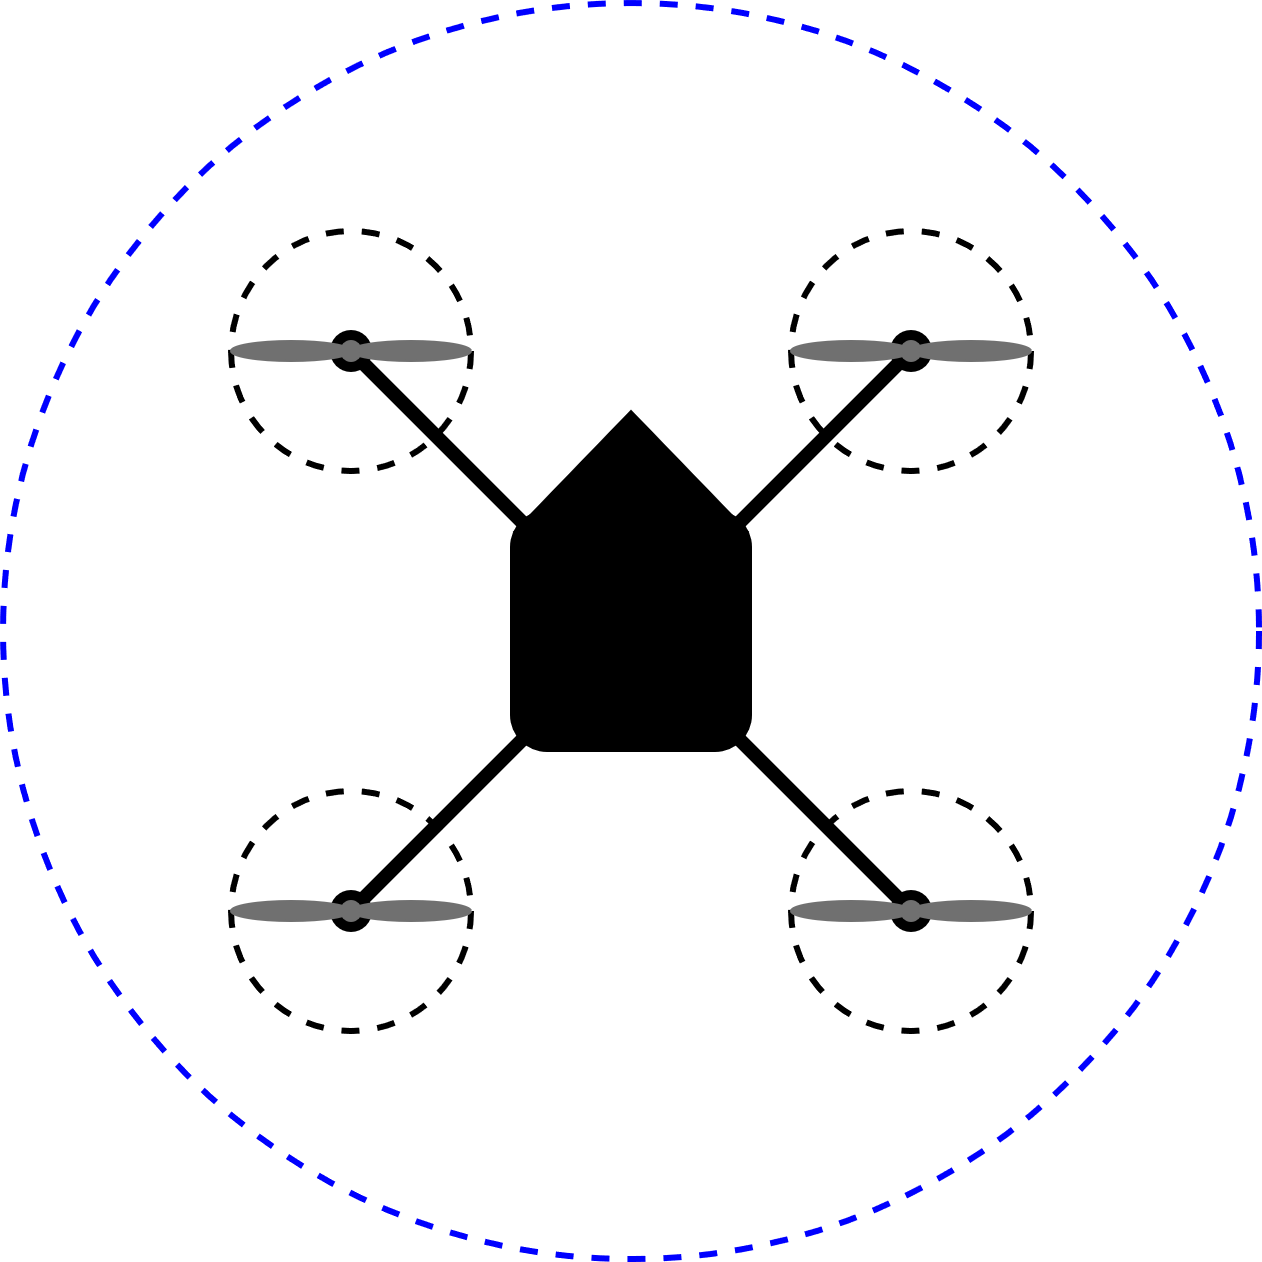
\includegraphics[width=0.35\textwidth]{figures/ch_intro/BobleOmDrone.png}
    \caption{illustration of a "safety bubble" around a drone.}
    \label{fig:introSaftyBobble}
\end{figure}
%%%%%%%%%%%%%%%%%%%%%%%%%%%%%%%





\section{Drones}\label{s:drones}
To start out this report, two questions should be resolved, what is a drone and what is it used for. 
A drone is also called a UAV, which is short for unmanned aerial vehicles. A drone can be controlled in different ways, by either software or remote controller. Drones are not exclusively unmanned flying vehicles, but can also be a driving vehicle. Drones is the definition of unmanned vehicles, in this report the word drones will be used for flying drones.   
A drone has mainly two ways it is designed, fixed wing and multirotor \cite{drones_type}. The two types can be seen in figure \ref{fig:drones_type}. To learn more about these two types, some of the applications for each of the types will be reviewed in the next section.

\begin{figure}[h]
\centering
    \begin{subfigure}[h]{0.45\textwidth}
        
\includegraphics[width=\textwidth]{figures/PA/Fixedwing.pdf}
        \caption{Example of a fixed wing drone}
        \label{fig:fixedwing}
    \end{subfigure}
    ~
    \begin{subfigure}[h]{0.45\textwidth}
        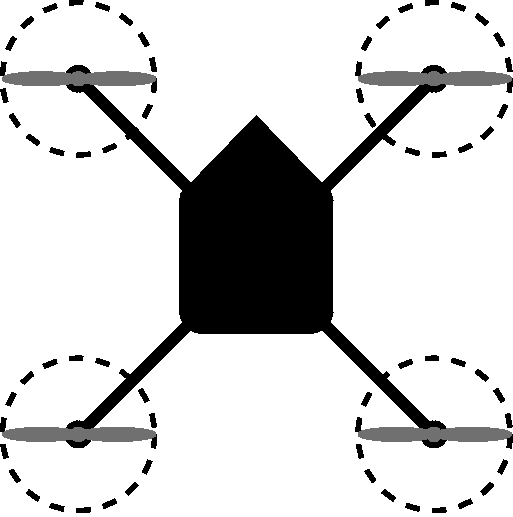
\includegraphics[width=\textwidth]{figures/PA/Quadcopter.pdf}
        \caption{Example of a multirotor drone}
        \label{fig:multirotor}
    \end{subfigure}
    \caption{Two types of drones}
    \label{fig:drones_type}
\end{figure}

 

%https://www.businessinsider.com/commercial-drone-uses-agriculture-business-military-2017-8?r=US&IR=T&IR=T
%\section{Drone applications}
%The use of drone in the industry and business has evolved a lot in the last few years, and the use evolves more each year. 
%The industries where drones are mostly used today are farming and military.
%\newline
%The use of drones in farming has evolved the traditional way of farming, as the drone can do things the farmer cannot do himself. The drones most used drone for farming, is multirotor drones. The drones can scan whole fields in minutes, and obtain knowledge of the crop's health. 
%\newline
%\newline
%The military has used drones since 1955, mainly for things where it is too dangerous for soldiers. This includes both combat missions and supervision. The military mostly use fixed wing drones because they are bigger and can carry a bigger cargo. They also have a much longer fly time. The fixed wing drone comes in all sizes, from small hand launched drones to large planes.
%\newline
%\newline
%It is not only in the farming industry and military drones have been used, or are being used.
%Drones is also being used for delivery of food and medicine to places where humans cannot get to. Such as areas where natural disasters have appeared, where the drones can give air support to the area \cite{drones_in_generel}.
%\newline
%In the future drones would be used to a lot more things, for example the multirotor drone will be used for exploration of mines and crash sites. Thus drones have to work in small and  narrow places, where they always have to know if it can fit. The multirotor drone will be used for this because it has a better mobility, than a fixed wing drone which needs a bigger space to fly. 










    \section{Drone applications}
The use of drones in the industry and business has evolved a lot in the last few years, and the use evolves more each year. 
The industries where drones are mostly used today are farming and military.
\newline
The use of drones in farming has evolved the traditional way of farming, as the drone can do things the farmer cannot do himself. The drones, that are most used for farming, is multirotor drones. The drones can scan a whole field in minutes, and obtain knowledge of the crop's health. 
\newline
\newline
The military has used drones since 1955, mainly for things where it is too dangerous for soldiers. This includes both combat missions and supervision. The military mostly use fixed wing drones because they are bigger and can carry a bigger cargo. They are also much more efficient, and therefore have a much longer fly time. The fixed wing drone comes in all sizes, from small hand launched drones to large planes.
\newline
\newline
It is not only in the farming industry and military drones have been used, or are being used.
Drones is also being used for delivery of food and medicine to places where humans cannot get to. Such as areas where natural disasters have appeared, where the drones can give air support to the area \cite{drones_in_generel}.
\newline
In the future drones would be used to a lot more tasks, for example the multirotor drone will be used for exploration of mines and crash sites. Thus drones have to work in small and narrow places, where they always have to know if it can fit. The multirotor drone will be used for this because it has a better mobility, than a fixed wing drone which needs a bigger space to fly.
    \section{Choice of drone}\label{s:vores_drone}
For the purpose of this project a multirotor drone will be chosen. The drone chosen for the project was a self built drone.
A Quanum Outlaw 270 Racing Drone Frame Kit with 305 mm in diameter was chosen as the main body for the drone system, the full drone is shown on figure \ref{fig:TheChosenOne}. The reason for choosing a larger drone body and the reason for more powerful motors will be used is because of the possibility of lifting a heavier payload, such as a micro controller and sensors. 

\begin{figure}[H]
    \centering
    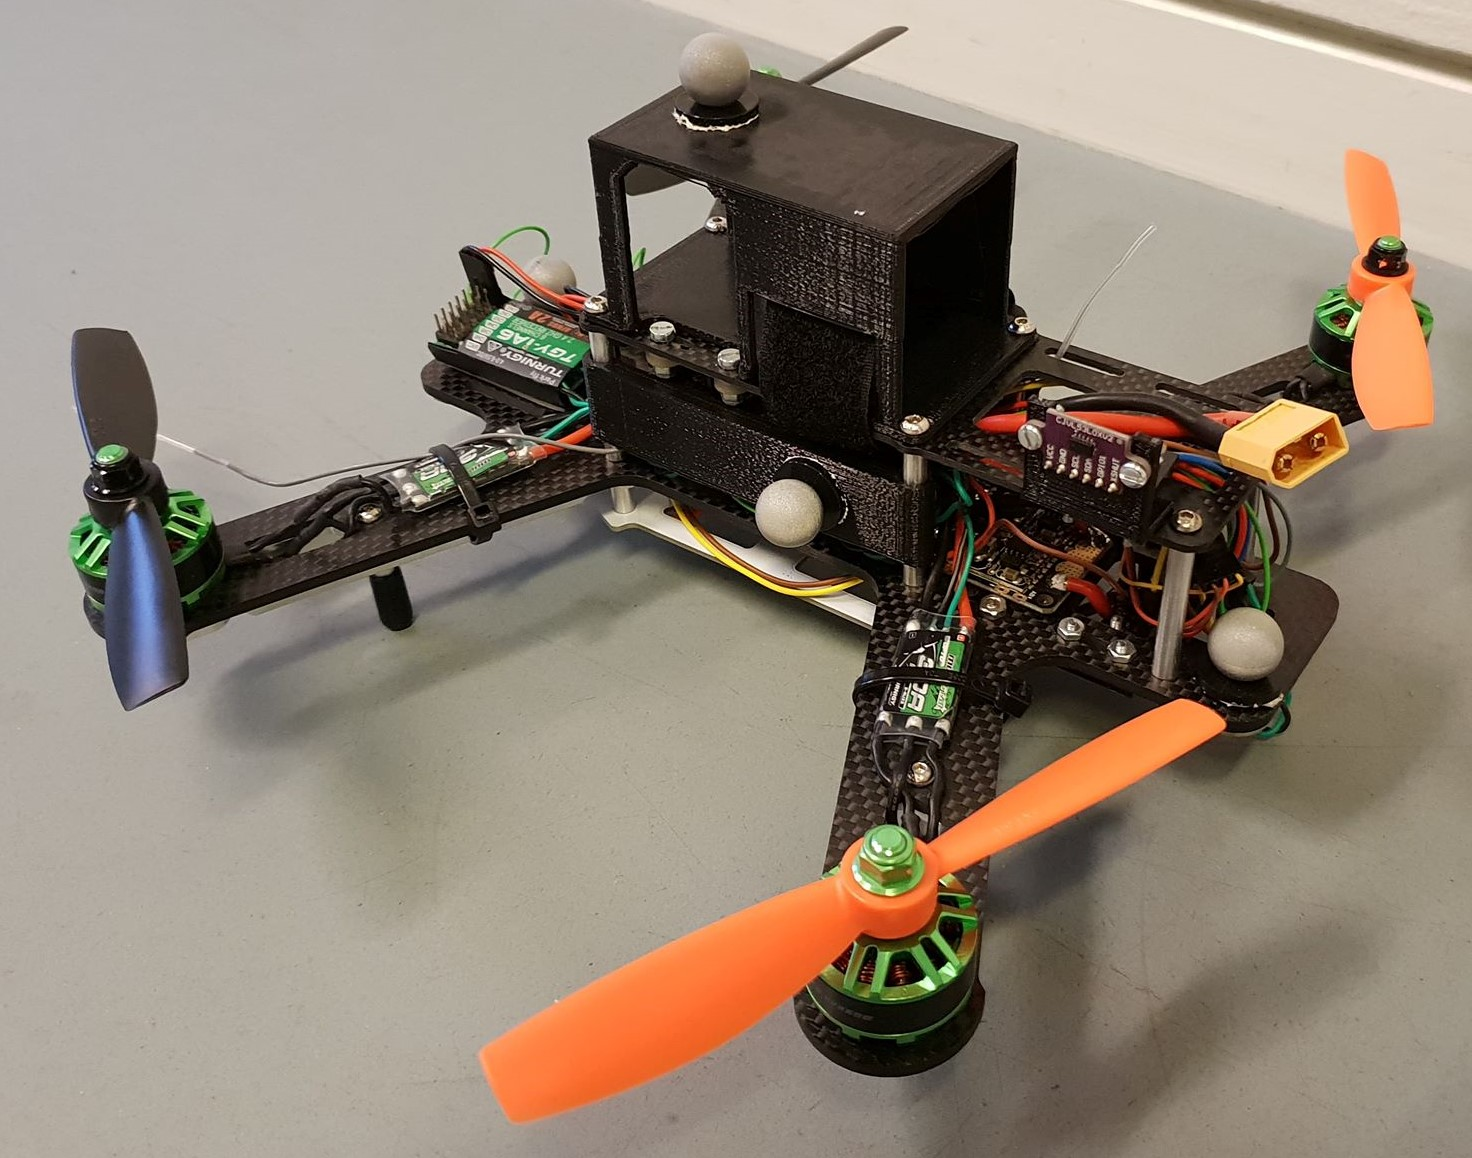
\includegraphics[width=0.5\textwidth]{figures/ch_intro/TheChosenOne2.jpg}
    \caption{A picture of the chosen drone for this project.}
    \label{fig:TheChosenOne}
\end{figure}

\subsection*{Composition of quadcopter parts}
The composition of the different parts on the quadcopter is illustrated on figure \ref{fig:blockdiagramDrone} and the list of components can be seen in the table \ref{tab:drone_element}. 

\begin{figure}[H]
    \centering
    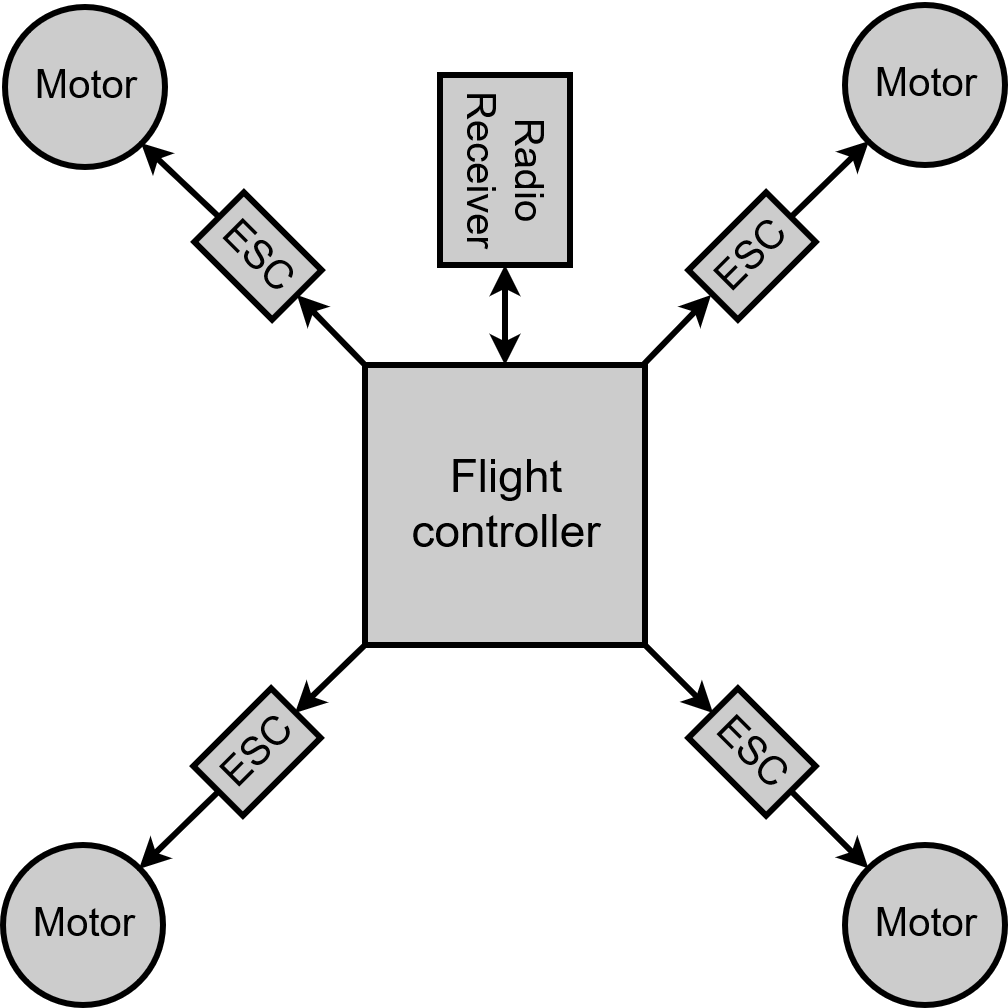
\includegraphics[width=0.5\textwidth]{figures/ch_intro/BlockdiagramOfTheDrone.png}
    \caption{Block diagram of the quadcopters individual parts connection.}
    \label{fig:blockdiagramDrone}
\end{figure}

\begin{table}[H]
\caption{List of the components used for the drone.}\label{tab:drone_element}
\begin{tabular}{|c|p{12cm}|}
\hline
\textbf{Quantity} & \textbf{Item} \\ \hline
1 x  & \textbf{Frame kit:} Quanum Outlaw 270 Racing Drone Frame Kit \\ \hline
1 x & \textbf{Flight controller:} Skyline32 Acro Flight Controller w/Baseflight  Cleanflight \\ \hline
4 x & \textbf{Motor:} MultiStar Viking 2206-2600kv Brushless Outrunner Drone Racing Motor (CCW) \\ \hline
1 x & \textbf{Battery} Turnigy Heavy Duty 2200mAh 4S 60C Lipo Pack w/XT60U Connector \\ \hline
1 x & \textbf{Controller unit} Turnigy TGY-i6 AFHDS Transmitter and 6CH Receiver (Mode 2) \\ \hline
4 x & \textbf{ESC:} Turnigy MultiStar 32bit 30A Race Spec ESC 2~4S NAKED (OPTO) \\ \hline
4 x & \textbf{Propellers:} Diatone Bull Nose Plastic Propellers \\ \hline
\end{tabular} 
\end{table}

    %\section{Drone movement}
%As mentioned before, this project involved the uses of drones, it is necessary to understand some theory of the physics for drones.
The type of multirotor drone that will be used in this project is a quadcopter \cite{PhysicsofDroneFlight}. A quadcopter is a drone with four rotors, as seen on figure \ref{fig:dronePhysics_1}.
\begin{figure}[H]
    \centering
    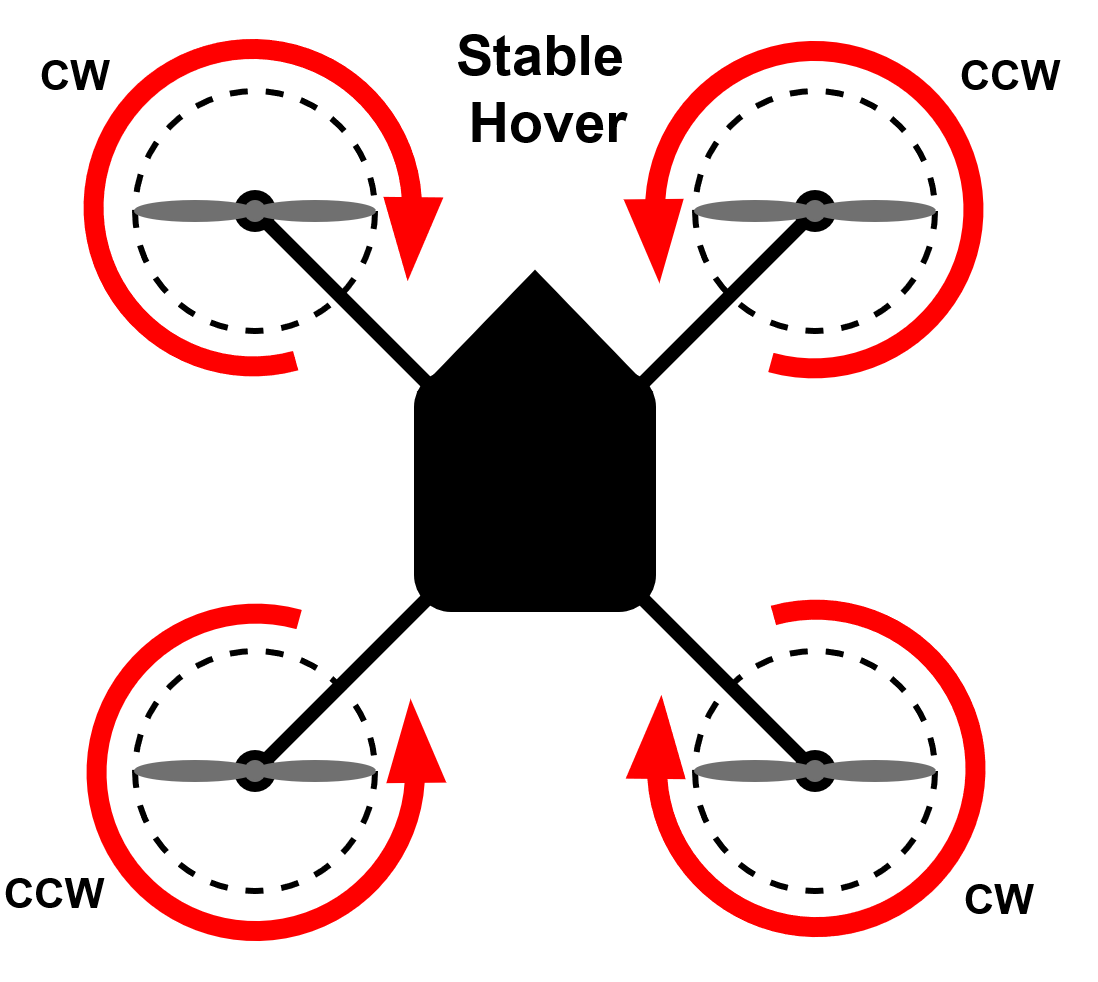
\includegraphics[width=0.4\textwidth]{figures/ch_intro/physics-of-multirotor.png}
    \caption{Illustration of a quadcopter when it is hovering.}
    \label{fig:dronePhysics_1}
\end{figure}
Two of the rotors are configured to rotate clockwise and the other two rotors are counter-clockwise. To control the drone’s movement, the speed of the rotors changes according to the desired action. The different types of movement a drone can do are hovering/altitude control, yaw, roll and pitch.
\newline
\newline
By rotating the rotors, a thrust will be created, see figure \ref{fig:QC_freeBodyDiagram}. This thrust will create a force upward $F_{Thrust}$. If this force are greater than the gravitational pull on the drone $F_g$, and all the rotors rotate has the same speed, it will increase the altitude of the drone. To get the drone to hover in the same position, the thrust must be the same as the gravitational force \cite{PhysicsofDroneFlight}.
\begin{figure}[H]
    \centering
    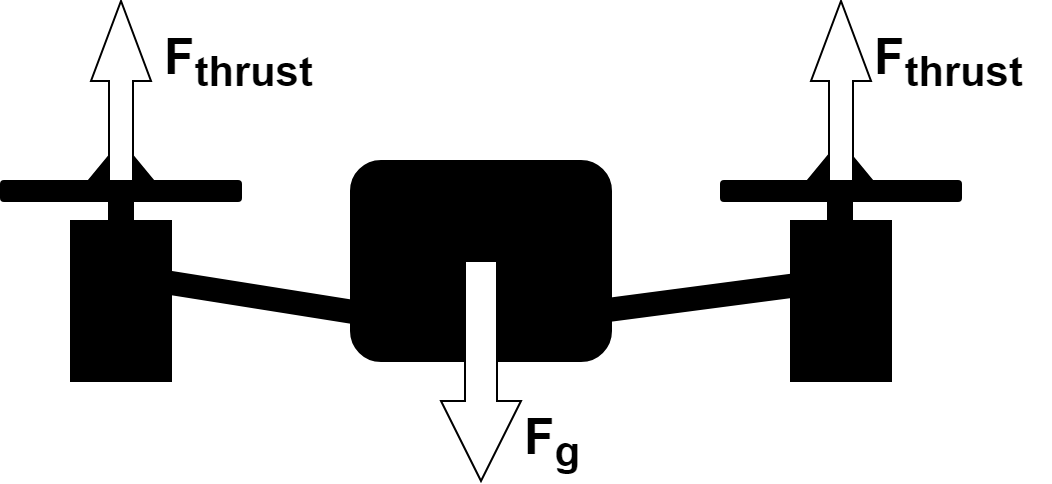
\includegraphics[width=0.45\textwidth]{figures/ch_intro/droen_frit_legeme-diagram.png}
    \caption{Free body diagram of a quadcopter.}
    \label{fig:QC_freeBodyDiagram}
\end{figure}
As mentioned previously, one of the movements of a drone is pitching. By pitching the drone, it will tilt either forward or backwards. By tilting the drone forward, it will make the drone fly forward. The illustration in figure \ref{fig:dronePhysics_2} shows, the drone can be moved forward by firstly decreasing the thrust of the two front rotors and increasing the thrust of the two back rotors. This will pitch the drone forward.
\begin{figure}[H]
    \centering
    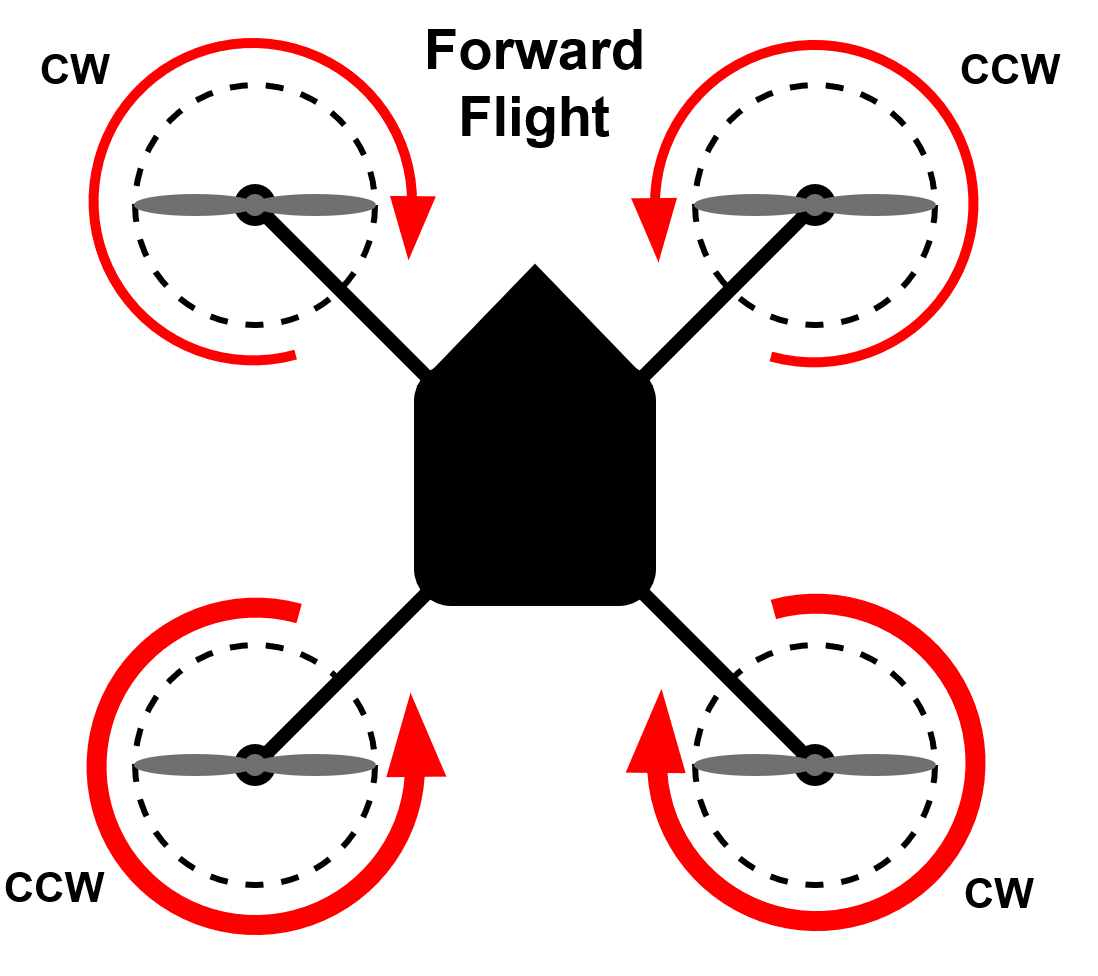
\includegraphics[width=0.4\textwidth]{figures/ch_intro/physics-of-multirotor-2.png}
    \caption{Illustration of a quadcopter when it is flying forward.}
    \label{fig:dronePhysics_2}
\end{figure}
After the drone have been pitch forward to a desired angle, all the rotors will then rotate with the same thrust, as when it's hovering but with a slightly higher thrust\cite{PhysicsofDroneFlight}.
\newline
Sideways movement is equivalent to moving forward and backwards. The different is that the drone is rolling instead of pitching. To roll/tilt the drone right, the two right rotors decreases its thrust and the left rotors increases its thrust, this can be seen on figure \ref{fig:dronePhysics_3}. After the drone have been tilted right, all the rotors will rotate with the same thrust, to fly right. 
\begin{figure}[H]
    \centering
    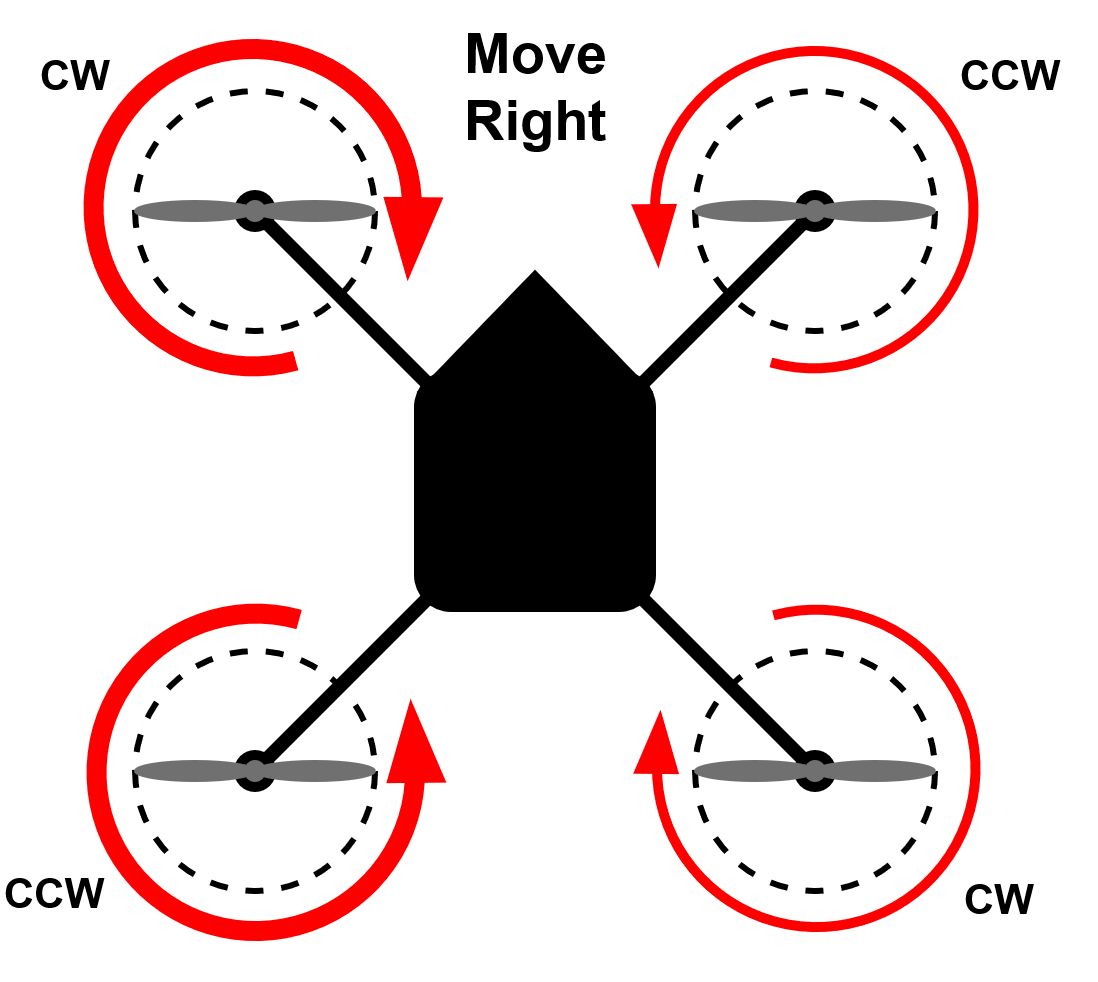
\includegraphics[width=0.4\textwidth]{figures/ch_intro/physics-of-multirotor-3.png}
    \caption{Illustration of a quadcopter when it is flying right.}
    \label{fig:dronePhysics_3}
\end{figure}

The last type of movement the drone can do is yaw/rotate. To understand how the drone can rotate, it is necessary to look into the rotors. When a rotor rotates, it generates a rotational force also known as torque. Because of the torque of a rotor that rotate clockwise, the drone will rotate counter-clockwise. By using a counter-clockwise rotor with the same force, the two opposite torque will cancel each other out\cite{PhysicsofDroneFlight}. This means that the drone does not rotate when tilting. The clockwise rotors are placed opposite of each other, and the same with the counter-clockwise, as it can be seen on figure \ref{fig:dronePhysics_4}.
\newline
\begin{figure}[H]
    \centering
    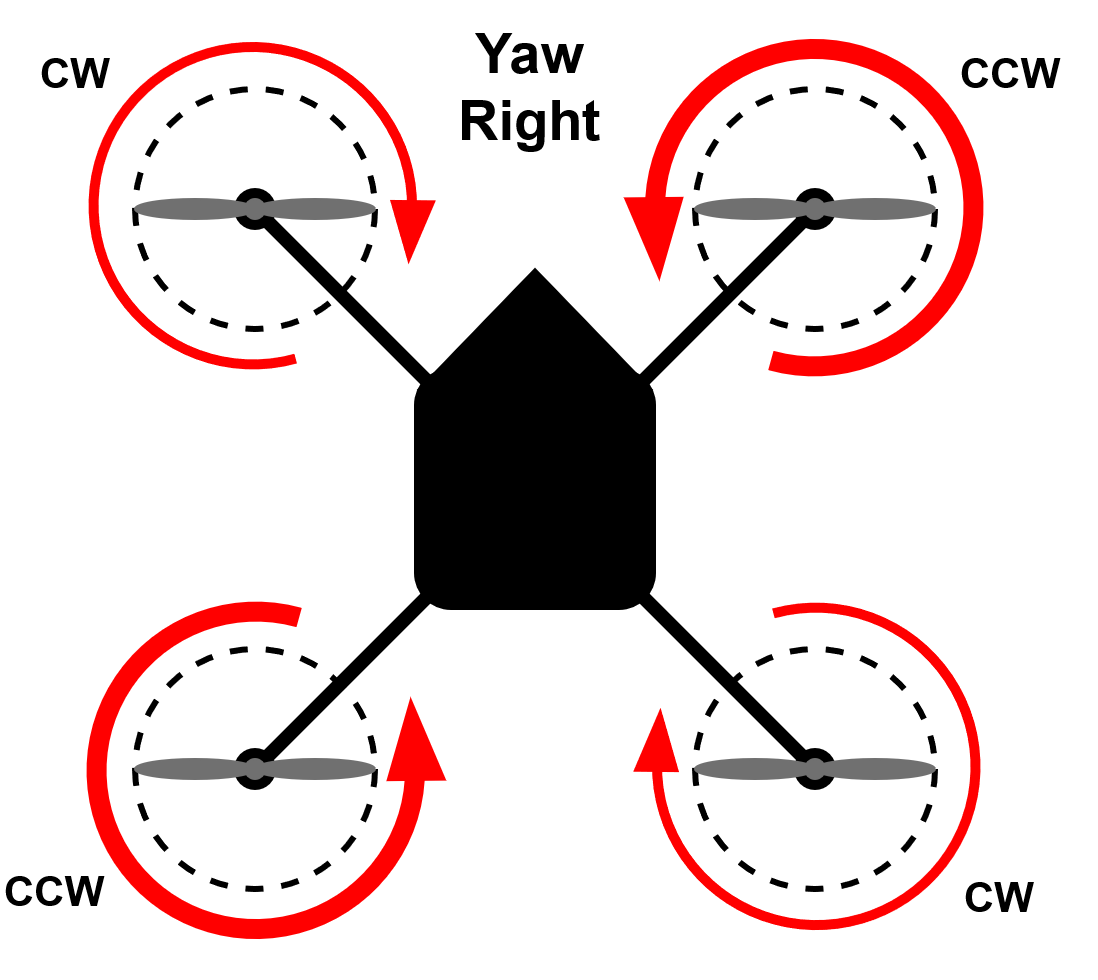
\includegraphics[width=0.4\textwidth]{figures/ch_intro/physics-of-multirotor-4.png}
    \caption{Illustration of a quadcopter when it is rotating.}
    \label{fig:dronePhysics_4}
\end{figure}
For the drone to rotate right the two counter-clockwise rotors must increase the thrust, from the hovering state, and the thrust of the clockwise must decrease, which can be seen in figure \ref{fig:dronePhysics_4}. When increasing and decreasing the thrust of the rotors, the total thrust must be the same as in hovering state for it not to lose or gain altitude. 
    \section{Initial Problem statement}\label{s:initial_problem}
How can a "safety bobble" be made for a off the shelf drone, so it is prevented to fly in to solid materials?
\newline
To gain the proper knowledge to solve this problem, it is first needed to have knowledge of how a drone move around in the air. Therefore the a drone's physics need to be explained.

    
%
%
%%%%%%%%% Problem analysis %%%%%%%%%%%%%%%%
\chapter{Problem Analysis}\label{ch:PA}
    In order to fly a drone indoors, there has to be a way to ensure that it doesn't collide with obstacles, and ensure that it can reliably navigate from its current position to a single, or a series of destinations. Usually this could be done by using GPS or similar systems, but indoors this isn't a reliable option as the signal is blocked by the building, and even if it was available, the precision would be too low to navigate hallways with.\\
This means another way to safely navigate a drone indoors has to be developed, preferably a self contained system making the drone independent on which building it's placed in.
In this project the group have decided to navigate indoors by using the walls and floor as reference surfaces.
    %\section{Quadcopter Components}
When building a quadcopter, it is necessary to understand which parts that are necessary in the build and their purpose for the quadcopter.
The different parts of a quadcopter, are frame/chassis, motors, Propellers, Electronic speed controller (ESC), flight controller, battery, and if you want to remote control it, a radio system.

%
%
\subsection{Frame}
 The frame of the quadcopter is the skeleton that holds all part of the drone and comes in different shapes. The shapes that have the most notable characteristics, are the H-frame and X-frame.
 \newline
 \newline
The H-frame shape drone have a design that make more space to mount more modules on the drone. It also has the benefit of  having the battery mounted at the top of the quadcopter. With the battery mounted at the top of the quadcopter it insures that the quadcopter does not land on the battery and by this the battery are better protected \cite{FPVFrame}.
\newline
\newline
When taking about a H-frame, there are different style such as a true H-frame or a HX-frame, this can be seen in figure \ref{fig:QC_HFrame}. In figure \ref{fig:QC_TrueH-Frame} a true H-frame can be seen, and are as the name implies, a quadcopter frame that shape look like a H, where the HX-frame is a X shapes frame that has the central body of a H-frame and can be seen in figure \ref{fig:QC_HXFrame}.
\begin{figure}[h]
    \centering
    \begin{subfigure}[b]{0.49\textwidth}
        \centering
        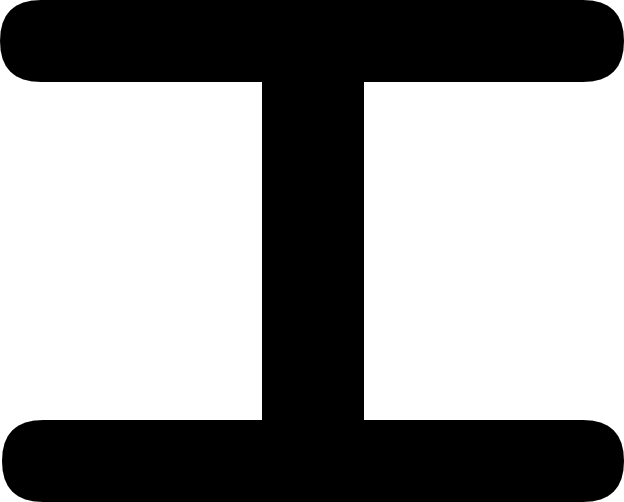
\includegraphics[width=0.5\textwidth]{figures/PA/QCComponent/H-shape.png}
        \caption{True H-shape frame}
        \label{fig:QC_TrueH-Frame}
    \end{subfigure}
    \begin{subfigure}[b]{0.49\textwidth}
        \centering
        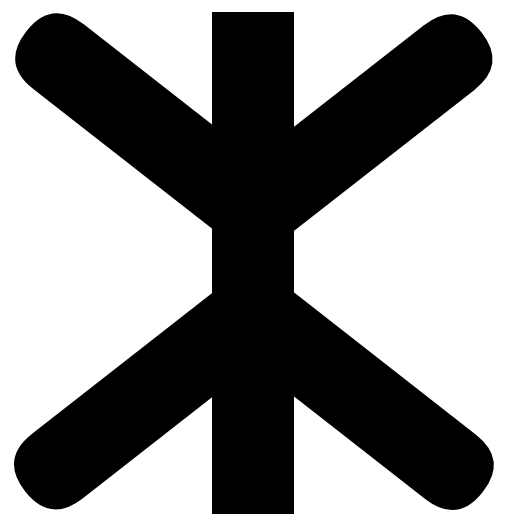
\includegraphics[width=0.5\textwidth]{figures/PA/QCComponent/HX-shape.png}
        \caption{HX-shape frame}
        \label{fig:QC_HXFrame}
    \end{subfigure}
    \caption{Two different style H-frame}
    \label{fig:QC_HFrame}
\end{figure}
\newline
The X-frame are a type of frame that, as the name implies, are a frame that has the shape of a X, as it can be seen in figure \ref{fig:QC_XFrame}. Because of the shape of the frame, there is less spaces to mount modules on, but this has the benefit of a lighter frame as is has no unnecessary weight. because the central body is smaller the battery will normally be mounted under the frame, which can damage the battery when landing, if landing on uneven terrain, with small feet.\cite{FPVFrame}.
\begin{figure}[h]
    \centering
    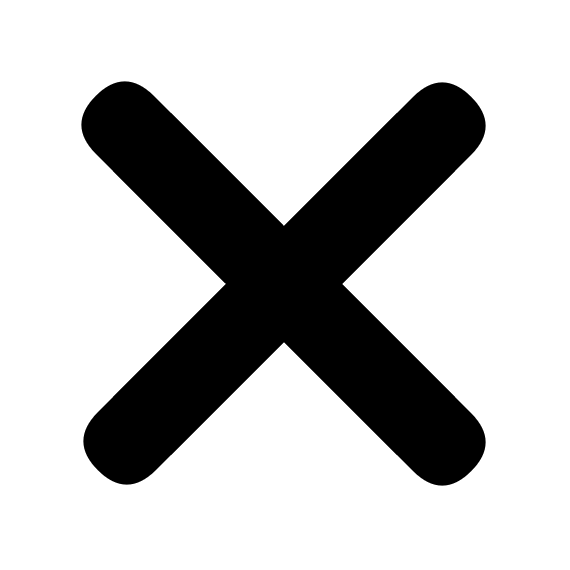
\includegraphics[width=0.3\textwidth]{figures/PA/QCComponent/X-shape_frame.png}
    \caption{X-shape frame}
    \label{fig:QC_XFrame}
\end{figure}
%
%
\subsection{Motors}
The next component a drone must use are motors, which are some of the more important components of the drone. The motors can be found in different types. The main motor type for drones would be Brushless DC Motors (BLDC), though brushed DC motors are also used on small drones. With BLDC motors for drones, there are two different variants Inrunners and outrunners. The inrunners are a type of motor, where it’s the outside of the motor that are still, and the rotor are in inside rotating. This type of motor has a higher rotation speed. The outrunner are the opposite of the inrunners as it’s the outside of the motor that’s rotating. This type is more common as it generates a higher torque to drive the propellers.
\newline
\newline
Motors are rated KV that stands for RPM per volt applied, which means that a higher KV will give a higher rotation speed \cite{DIYDrone}. Motors are also sold as clockwise and counter-clockwise, where a quadcopter needs 2 of each.

%
%
\subsection{Propellers}
The component that can have the highest effect on the thrust of the motors are the propellers. By increasing the size, more trust will be created at the same RPM, however more torque is also required. Thus, propeller size and motor rpm has to be matched. The measurements that the propellers are measured with are the diameter and the pitch. the diameter of the propeller is the length of them and are measured in inches.\\
The pitch of a propeller is the distance it would move in one rotation, if thought of as a screw. \cite{DIYDrone}.

%
%
\subsection{Electronic speed controller}
To control the speed of which the motors are spinning four electronic speed controllers or short ESC’s are used, one for each motor \cite{QuardcoptorParts}. 

On most RC vehicles, ESCs are 3-phase Variable Frequency Drives (VFD), as BLDC motors require 3 phase AC to be driven. 

When deciding which ESC that should be used of the quadcopter, the highest current draw of the motors is determined, and an ESC that has a value of it or higher is chosen \cite{DIYDrone}.

%
%
\subsection{Flight controller}
the brain of the quadcopter is the flight controller, which is a small computer that controls it. The flight controller has some in-build sensors such as gyroscopes and accelerometer to detect changes of the drone and control the motors, so the quadcopter stays in the air. the component that gets commands from the user are also the flight controller. A flight controller can also have inbuild barometric pressure sensors and magnetometer and are a hub so other components such as GPS or external sensors can be connected \cite{FlightController}.

%
%
\subsection{Battery}
The type of battery almost all quadcopters uses are LiPo batteries, as it has a high discharge rate. A problem with  using this type of battery is that they have are rather sensitive for overcharging and over-discharging. In these cases, hydrogen and heat is formed, which can lead to the battery 'puffing' or even bursting into flames.\\
Because of this, safety measures have to be taken when handling these batteries, especially when charging them as this is often a lengthy process, meaning it can't be fully supervised.\\
Some of the safety measures recommended when charging this type of battery, are to keep the them in a fire-safe bag when charging them, so if the battery burst in to flames the bag can contain it, and using a proper LiPo charger, not exceeding the max charging rate of the battery. 
\cite{DIYDrone}.

%
%
%\subsection{receiver transmitter} skal det med
    \section{Drone movement}
%As mentioned before, this project involved the uses of drones, it is necessary to understand some theory of the physics for drones.
The type of multirotor drone that will be used in this project is a quadcopter \cite{PhysicsofDroneFlight}. A quadcopter is a drone with four rotors, as seen on figure \ref{fig:dronePhysics_1}.
\begin{figure}[H]
    \centering
    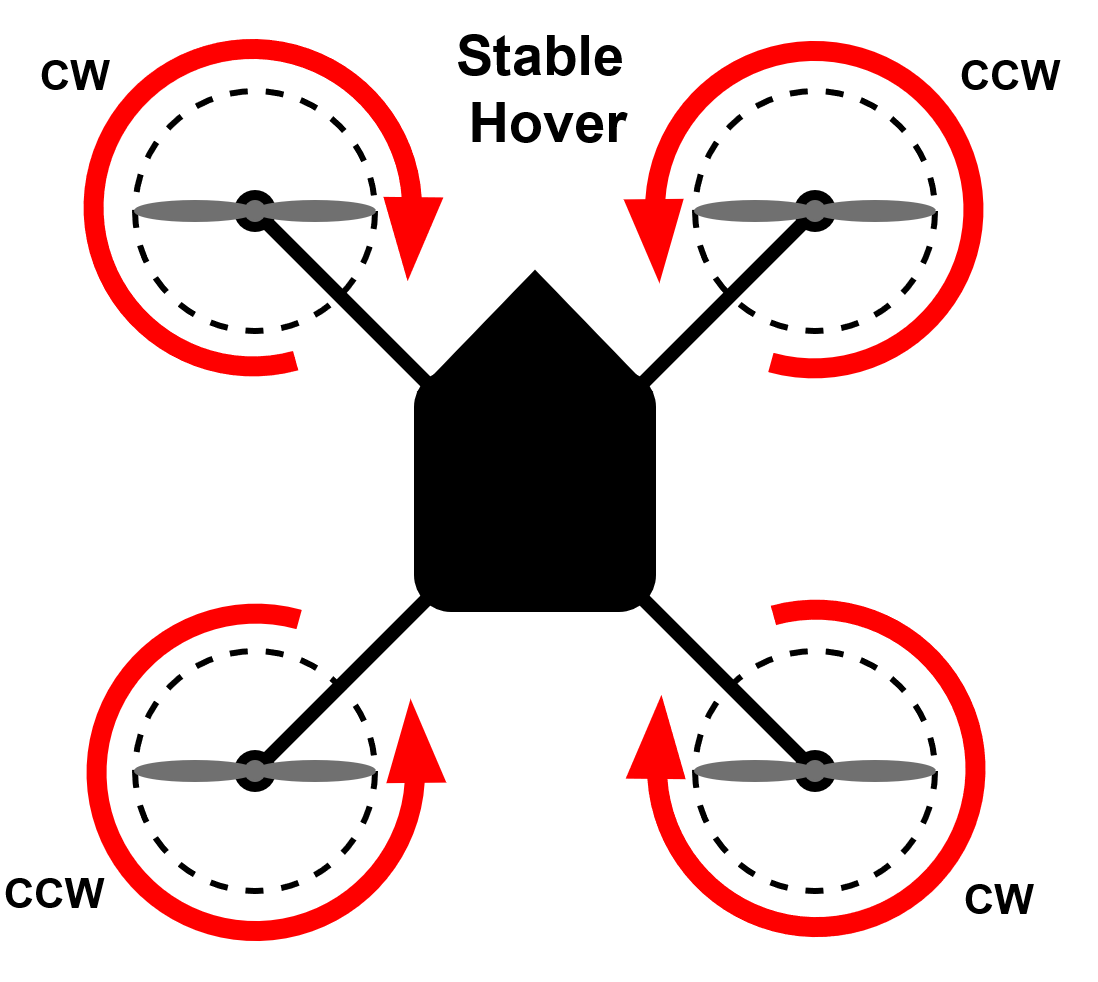
\includegraphics[width=0.4\textwidth]{figures/ch_intro/physics-of-multirotor.png}
    \caption{Illustration of a quadcopter when it is hovering.}
    \label{fig:dronePhysics_1}
\end{figure}
Two of the rotors are configured to rotate clockwise and the other two rotors are counter-clockwise. To control the drone’s movement, the speed of the rotors changes according to the desired action. The different types of movement a drone can do are hovering/altitude control, yaw, roll and pitch.
\newline
\newline
By rotating the rotors, a thrust will be created, see figure \ref{fig:QC_freeBodyDiagram}. This thrust will create a force upward $F_{Thrust}$. If this force are greater than the gravitational pull on the drone $F_g$, and all the rotors rotate has the same speed, it will increase the altitude of the drone. To get the drone to hover in the same position, the thrust must be the same as the gravitational force \cite{PhysicsofDroneFlight}.
\begin{figure}[H]
    \centering
    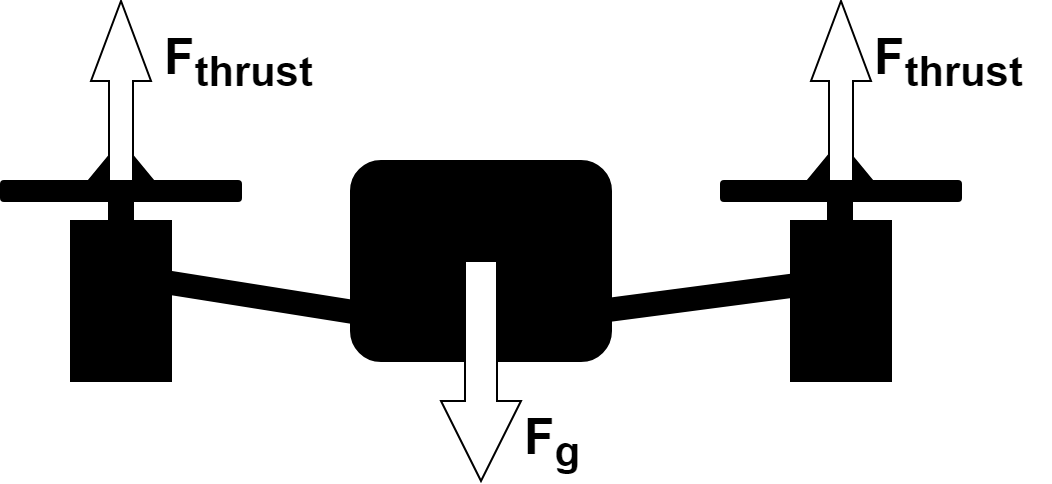
\includegraphics[width=0.45\textwidth]{figures/ch_intro/droen_frit_legeme-diagram.png}
    \caption{Free body diagram of a quadcopter.}
    \label{fig:QC_freeBodyDiagram}
\end{figure}
As mentioned previously, one of the movements of a drone is pitching. By pitching the drone, it will tilt either forward or backwards. By tilting the drone forward, it will make the drone fly forward. The illustration in figure \ref{fig:dronePhysics_2} shows, the drone can be moved forward by firstly decreasing the thrust of the two front rotors and increasing the thrust of the two back rotors. This will pitch the drone forward.
\begin{figure}[H]
    \centering
    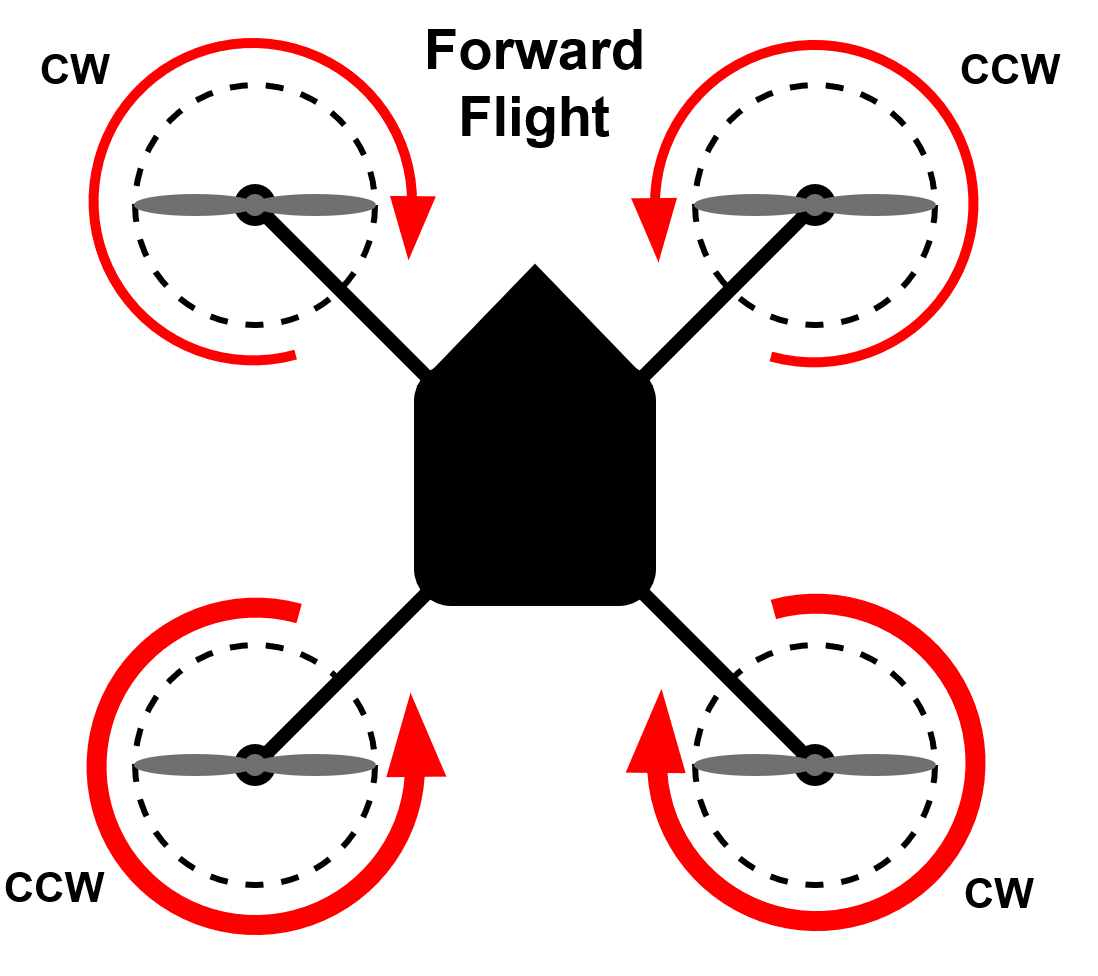
\includegraphics[width=0.4\textwidth]{figures/ch_intro/physics-of-multirotor-2.png}
    \caption{Illustration of a quadcopter when it is flying forward.}
    \label{fig:dronePhysics_2}
\end{figure}
After the drone have been pitch forward to a desired angle, all the rotors will then rotate with the same thrust, as when it's hovering but with a slightly higher thrust\cite{PhysicsofDroneFlight}.
\newline
Sideways movement is equivalent to moving forward and backwards. The different is that the drone is rolling instead of pitching. To roll/tilt the drone right, the two right rotors decreases its thrust and the left rotors increases its thrust, this can be seen on figure \ref{fig:dronePhysics_3}. After the drone have been tilted right, all the rotors will rotate with the same thrust, to fly right. 
\begin{figure}[H]
    \centering
    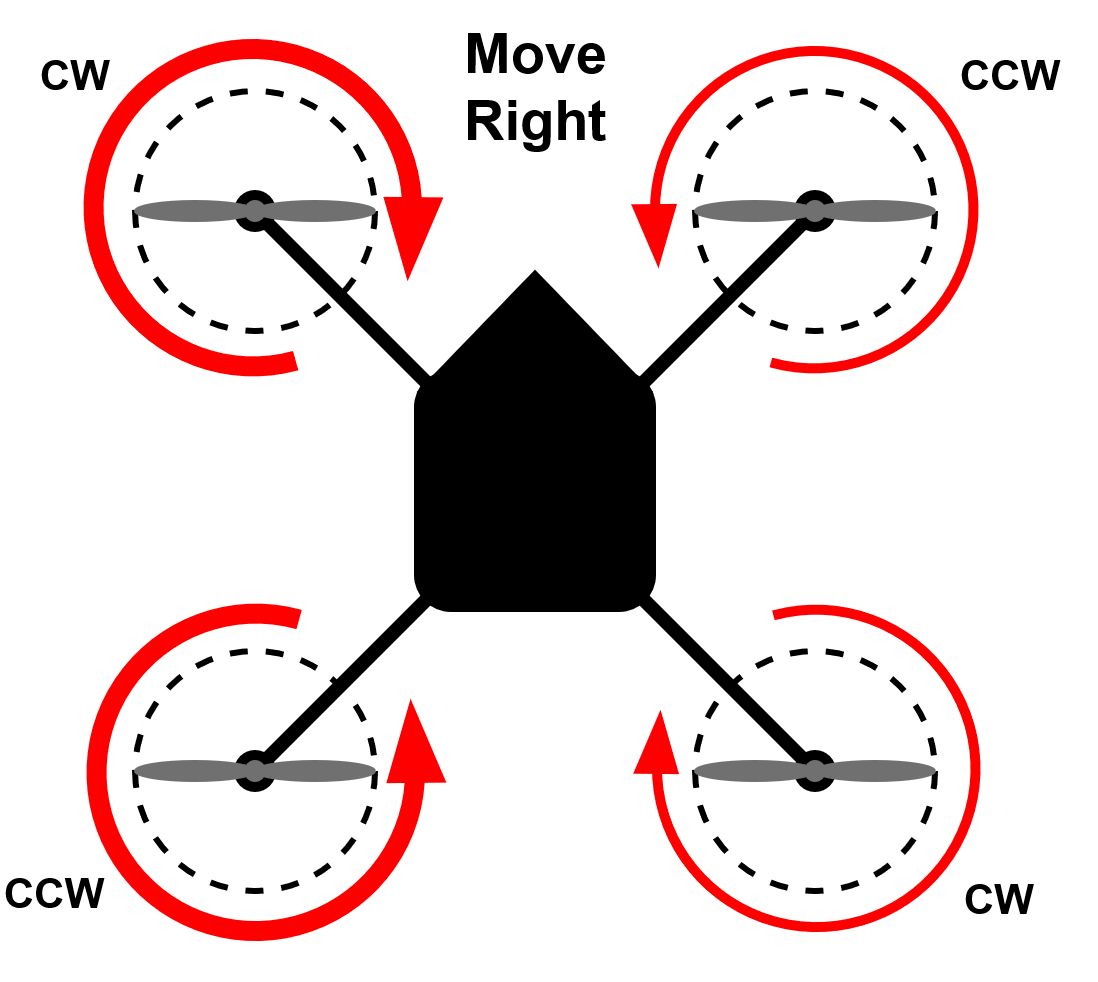
\includegraphics[width=0.4\textwidth]{figures/ch_intro/physics-of-multirotor-3.png}
    \caption{Illustration of a quadcopter when it is flying right.}
    \label{fig:dronePhysics_3}
\end{figure}

The last type of movement the drone can do is yaw/rotate. To understand how the drone can rotate, it is necessary to look into the rotors. When a rotor rotates, it generates a rotational force also known as torque. Because of the torque of a rotor that rotate clockwise, the drone will rotate counter-clockwise. By using a counter-clockwise rotor with the same force, the two opposite torque will cancel each other out\cite{PhysicsofDroneFlight}. This means that the drone does not rotate when tilting. The clockwise rotors are placed opposite of each other, and the same with the counter-clockwise, as it can be seen on figure \ref{fig:dronePhysics_4}.
\newline
\begin{figure}[H]
    \centering
    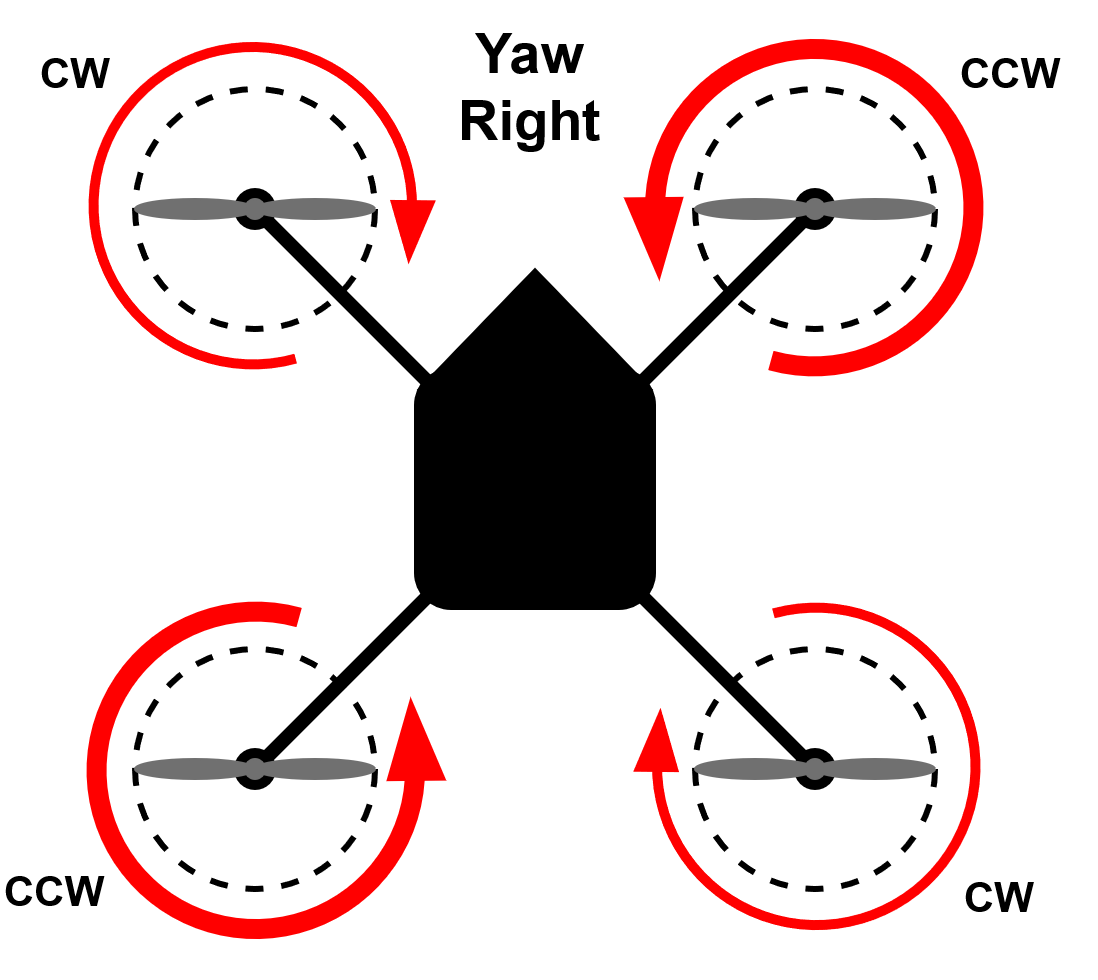
\includegraphics[width=0.4\textwidth]{figures/ch_intro/physics-of-multirotor-4.png}
    \caption{Illustration of a quadcopter when it is rotating.}
    \label{fig:dronePhysics_4}
\end{figure}
For the drone to rotate right the two counter-clockwise rotors must increase the thrust, from the hovering state, and the thrust of the clockwise must decrease, which can be seen in figure \ref{fig:dronePhysics_4}. When increasing and decreasing the thrust of the rotors, the total thrust must be the same as in hovering state for it not to lose or gain altitude. 
    \section{Control Units}\label{s:cont}
Before it is possible to fly the drone up in a certain altitude and move it around in the four directions, a method of controlling the drone is necessary. The drone can either be controlled with a remote control unit or by on-drone software. %hard coded to follow a path. 
\newline
There are different options when it comes to controlling the drone with a control unit. It is firstly important to understand how communication between a drone and a control unit works. %drone controlling works.

The communications works by the control unit having a built-in transmitter. By using a control unit the transmitter can transfer control data to the drone. The data could be anything that the user presses on the control unit. When the data are sent, the built-in receiver on the drone, will receive all the data from the control unit. To use this method it is important the control unit and the drone are connected to each other \cite{Control}.
%The way the user communicates with the drone is by sending data to the drone with a transmitter like a remote control. The data will be received by the receiver equipped on the drone, and the drone will respond to it. \cite{control}



The control units there are most used for drones are handheld remote controllers, using either Bluetooth, Wi-Fi or a proprietary RF protocol.

\subsubsection*{Proprietary RF}
%As the name also says 
The communication between the transmitter and receiver is carried out over a proprietary RF protocol, commonly in the license free 2.4GHz frequency band. Transceivers of this type often incorporate frequency hopping and error correction, and high powered transmitters, to ensure a stable, long range connection can be maintained. 

\subsubsection*{Bluetooth/Wi-Fi controllers}
The drone can also be controlled via an application using Bluetooth or Wi-Fi compatible devices like smartphones and tablets. Manufactures of drones like DJI have developed an application that gives advanced positioning, first person video controls, programmable flight routes, and much more. The downsides of using Bluetooth or Wi-Fi as a communication method, are the lack of a standard protocol for control drones and the short range \cite{droneRange}. 

Wi-Fi provides the ability to transmit larger amounts of data to and from the drone within a specific radius. The problem with using Wi-Fi is the short range of communication, in many cases lose connection. 

\subsection*{Autonomous drone control}
A way for the drone to fly automatically is by using Global Position system (GPS), it gives the ability such as auto pilot features, since it provides the drone with accurate position data.
Since the GPS is limited for outdoor applications, it is not useable indoors, and there are not many companies that have attempted to develop alternative systems for indoor purposes. An example of an indoor positioning system is GT-position from Gamesontrack \cite{gt-position}. 

GT-position indoor positioning-system uses Gameontracks own indoor satellites.
Based on a combination of radio and ultrasound they provide precise distances to any moving or stationary unit which has a sender in the system.
The satellites provide precision up to 10 mm and can measure up to 8 m distance. Satellites are combined in scenarios of 2, 3 or more which together form a 2D or 3D position in a coordinate system. More scenarios can be combined to extend coverage \cite{gt-position}.

\subsection*{Conclusion} 
For the purpose of this project RF controller will be used, because it exposes a standardized interface which can be broken into. The drone chosen for this project is equipped with an RF reciever, which can communicate with the RC transmitter in the controller \cite{Control}. Also mentioned earlier, by controlling the drone with RF, it provides control of the drone for a much greater distance than a Wi-Fi or Bluetooth connection.












    \section{Problem statement}\label{s:problem_statment}
Now when the normal methods of controlling the drone have been explained, it shows that there is a need of more usable solutions to make the "safety bobble" around the drone. To make the problem more solvable a small downsizing is needed, so if the drone can hold a specific distance to a wall or floor and follow it, it should be enough as a proof of concept.
\newline
So the problem that needs solved goes as:
How can a device be implemented on a of the shelf drone, so it is capable to hold a specific distance to a wall and follow it as well?

%This project will focus on how to develop a remote controlled indoor drone with stability features. To avoid as many collisions as possible the drone will maintain a specific distance and angle to the wall and the ceiling . 
    \section{Navigation} \label{s:navi}
To make it possible to navigate a drone indoors, there are obstacles which are needed to be considered. There are two types of obstacles, permanent and temporary. The permanent obstacles can be the following; walls, ceiling, doors, windows and furniture. Temporary obstacles are objects like people or things placed in the path temporarily. This means it is necessary to avoid any collision with any humans and other objects, that can occur suddenly in front of the drone. The drone should be capable of detecting those obstacles. 
\newline

The drone needs to have different sensors to detect the obstacles. Some sensors that can be used in these situations are distance sensors. The drone need a minimum number of distance sensors to cover all the surroundings, as shown on figure \ref{fig:drone_sensor}.
\begin{figure}[H]
    \centering
    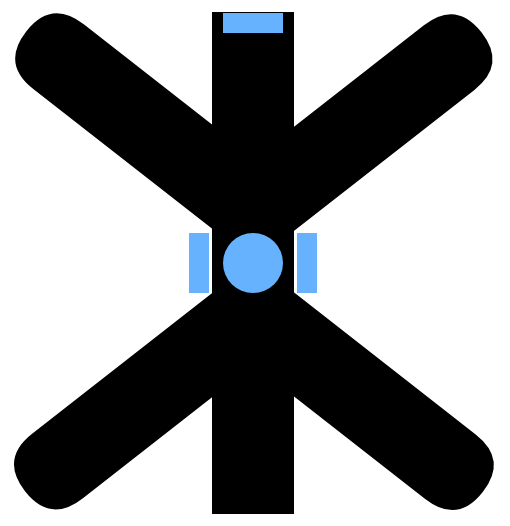
\includegraphics[width=0.3\textwidth]{figures/Navigation/DroneIR.png}
    \caption{Illustration of where the sensors can be placed on the drone.}
    \label{fig:drone_sensor}
\end{figure}
There are different sensors there can use to navigating a drone indoors. Sensors like Infra Red, Ultrasonic and Vision will be explained in the following sections.

\subsection*{Infra Red sensor}
One of the possible sensors are IR sensors, which is used in different devices such as laser distance meter. An IR sensor consists of an IR transmitter and an IR receiver. 
The IR sensor works by the transmitter flashing an infrared light out, when the light hits a surface, the light gets reflected back to the sensor's receiver. The distance then gets calculated from the time of flight, this is the time from when the light is flashed and to the sensor registers it again.


There are some disadvantage with IR sensors, which can be light distortion and different materials could reflect the light differently, this could interfere with the sensor measuring.
\newline
Ultrasonic sensors works the same as the IR sensors, the only difference is it uses ultra sound instead of infra red light.

\subsection*{Vision sensor}\label{ss:camera_pa}
Vision sensors consist of an image sensor that take images of their field of vision. These images can then be processed by a computer vision algorithm, to classify objects and avoid them.

The images can both be normal images captured with a normal image sensor, or the system could use Time of Flight depth image sensors, and get even more information for object classification

The main disadvantage of such a system, is the high complexity of both the hardware and software required. Such a vision system would require power full hardware to do real time image recognition, and the complexity of the software is outside the scope of this project.

\subsection*{Conclusion}
From the problem analysis it can be concluded that, a time-of-flight sensor will suit this project best. It is simple to implement and a good reliable sensor type. The only problem with it, is the time it takes before having the distance. To prevent this a good sampling time is needed, to make it possible to be used for checking distances to a surface.
\newline
To make the sampling time as small as possible an IR sensor have been chosen, these type of sensors have a much faster sampling time then a ultrasonic sensor.







    

%
%
%%%%%%%%% Requirements %%%%%%%%%%%%%%%

    \chapter{Requirements}\label{ch:Req}
The requirements that have been chosen for this project is listed in the following tabular \ref{tab:req}.  

\begin{table}[H]
\caption{Table of requirements.}\label{tab:req}
\begin{tabular}{|c|l|c|c|}
\hline
\textbf{Number} & \textbf{Performance requirements}  & \textbf{Desired value}& \textbf{Accuracy} \\ \hline
1 & Desired distance to a surface             & 400 mm       & $\pm$5 \% \\ \hline
2 & Detection of an object                    & $\geq$1000 mm      & -  \\ \hline
3 & Activation of the sensor at desired angle & $0\degree$          & $\pm10 \degree$  \\ \hline
4 & Drone speed                               & $\leq$ 1 m/s &   \\ \hline
 & \textbf{Functional requirements}  & \textbf{Desired value} & \\ \hline
5 & Overshoot              & $\leq$30 \% & \\ \hline
6 & Settling time           & $\leq$10 s & \\ \hline
7 & Steady state            & $\pm$5 \% & \\ \hline
8 & Sampling time          & $\geq$40 Hz   & \\ \hline
\end{tabular}
\end{table}

\section{Performance requirements} \label{sec:req}
In this section the requirements for performance that have been chosen, can be seen in table \ref{tab:req}, will be explained. %First the performance requirements and then the functional requirements. 

\begin{figure}[h]
    \centering
    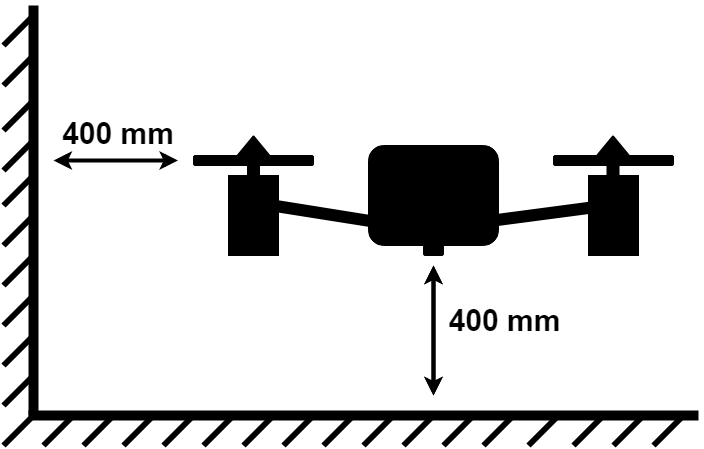
\includegraphics[width=0.70\textwidth]{figures/ch_req/figure_requirements.png}
    \caption{Figure of the requirements for the distance from the drone.}
    \label{fig:req_fig}
\end{figure}

%\subsection*{Desired distance to the floor}
%The distance to floor as seen in the table \ref{tab:req} is a fixed distance, as it is within the stable range of our sensors.


%The desired distance as seen in the table \ref{tab:req} is set,because it is necessary to avoid collision with any obstacles the drone meets on its route. These obstacles could be anything that are placed on the floor, an example of objects could be bags, chairs etc. But there are probably still some obstacles that the 400 mm might not be enough to avoid collision. However, this is just a proof of a concept, such that it would be possible to fly along side a even surface. 

%As shown in table \ref{tab:req} number 1, the desired fixed distance to the floor is 400 mm. The reason for a fixed distance is to avoid any collision with obstacles like lamps that are mounted in the celling.%The drone will avoid collision with objects like lamps in the ceiling by flying at a height at 400 mm.
%However, this is made as a proof of a concept, to make the drone fly along side a even surface. 
\subsection*{Desired distance to a surface}
The distance to a surface is set to 400 mm as a fixed distance. The distance is from the tip of the propellers to surfaces beside the drone, as shown on figure \ref{fig:req_fig}, and from the tip of the legs to the surface below, also shown on the figure \ref{fig:req_fig}. This is chosen such that the distance to the surfaces are far enough to avoid collision with either of the surfaces, and if the overshoot get to the maximum and even goes beyond that. 

\subsection*{Detection of an object}
The desired distance for detection an object is set to 1000 mm. Since the drone must be able to detect an object before the distance to the object reach the 400 mm, which is the desired distance to an object or surface. The detection of an object has been chosen to be at 1000 mm, to make it possible for the drone to stop before collision, at a reasonable speed.% From the datasheet it can be seen that the maximum distance for the chosen sensor to detect an object is 2000 mm, this mean by choosing 1000 mm it will be within the sensors range.

\subsection*{Activation of the sensor at desired angle}
The measuring angle from the sensor to the wall is chosen to be $0\degree$ with $\pm 10 \degree$. It is needed to make some variation from the $0\degree$ to make the sensor detect an object even when it is not perpendicular to the object. Therefor it is chosen to be at $\pm 10 \degree$ accuracy.

\subsection*{Drone speed}
The speed for the drone is limited to 1 m/s, this is chosen, because this will make the drone fly slowly enough to make a proof of concept for this project. This will also make it possible to follow the drones movement, and to stop within one meter. This means the drone should be able to decelerate at a rate of 1 m/s$^2$.

%The speed of the drone is limited to 1 m/s, so the drone flies slowly enough to make a proof of concept for the project. And it is still possible to follow the drones movements.

\section{Functional requirements}
Like the performance requirements were explained in \ref{sec:req}, will the focus in this section be on explaining the functional requirements.

\subsection*{Overshoot}
The overshoot of $\leq$ 30 \% is chosen to make sure the drone does not collide with an object, even if the desired distance to the wall fails. By using the 30 \% means that the distance accepted for the drone to move inside the desired distance will be at 120 mm. 
Since the overshoot and dampings ratio are dependent on each other, the overshoot can be used to find the damping ratio seen in equation \ref{eq:damping}. Where PO is the Percent Overshoot, these means the damping ratio will be 0.374 as shown in equation \ref{eq:damping}.
\begin{equation}\label{eq:damping}
   \zeta = \sqrt{\frac{(ln(\frac{\text{PO}}{100}))^{2}}{\pi^{2}+(ln(\frac{\text{PO}}{100}))^{2}}} \to \sqrt{\frac{(ln(\frac{\text{30}}{100}))^{2}}{\pi^{2}+(ln(\frac{\text{30}}{100}))^{2}}}=0.374
\end{equation}
\subsection*{Settling time}
The settling time is set to $\leq$10s, this time has been chosen to make sure the drone has time to settle in to its desired distance to a surface. It makes it possible to adjust the drones position. 
\subsection*{Steady state}
The steady state is set to  $\pm$5 \%, as it also is the accuracy to the desired distance to the wall. This also means that the steady state also need to be at this value. 

\subsection*{Sampling time}
The sampling time is set to 40 Hz, to make sure that there are enough sampling to ensure the phase offset caused by the sampling time, is not too big.

\section{Testing of the requirements}\label{s:test_requirements}
To make sure the drone lives up to all the requirements, some test specification is needed for each of the requirements.


For requirement number one and two, as it can be seen in table \ref{tab:req}. They are each tested at the maximum distance, specified by the requirements. Additionally they are also tested at 400 mm, to make sure they hold the $\pm5 \%$ to the specific distance. 


To make sure the sensors fulfill the third requirement, is to test if the sensor still can detect an object even if the sensor is not facing the wall directly, so to test this the sensors are each turn $\pm10\degree$ from the test object.


To test the fourth requirement, the drone's speed the drone's position over time needs to be tracked.


To make sure that requirement five, six and seven are fulfilled, each of these are first simulated and then tested. To test these requirements the drones position over time will again need to be tracked, and then processed to make sure the requirements are met. 


To make sure the sampling time meets requirement number eight, a number of samples is counted and the time used is noted. By using 
these two numbers the sampling time can be calculated. 
% overshoot(%) < (distance to ground(%)) from ((max measure distance) - (distance to ground))

% Settling time: vi skal vælge en tid (for stor stettling time kan få systemet til at virke langsomt.

% Steady state error: vælges ud fra afstandes sikkerhed

% krav til hvor meget fejl som vinkel for dronen må have

% SAMME KRAV TIL VÆG
%%%%%%%%%%%%%%%%%%%%%%%%%%%%%%%%%%%%%%%%%%%%%%%%%%%%%%%%%%%%%%%%%%%%%%%%%%

%%%%%% Krav til sensor %%%%%%%%%%%%%%

% krav til hvor præcis den er.

% krav til hvor hurtige den er til læse målte værdier.

% Krav til min afstand og max afstand.


%%%%%%%%%%%%%%%%%%%%%%%%%%%%%%%%%%%%%%%%%%%%%%%%%%%%%%%%%%%%%%%%%%%%%%%%
%%%%%%%%%%% Funktional krav %%%%%%%%%%%%%%%%%%%%%%%%%%

% Krav hvornår sensoren skal aktiveres

% Krav Krav til hvilke vinkel den må aflæse værdi fra væg og gulv.

% 

%%%%%%%%%%%%%%%%%%%%%%%%%%%%%%%%%%%%%%%%%%%%%%%%%%%%%%%
% det er ikke et krav hvis dataene er taget fra et datasheet. (det er limitations)

% hvordan skal kravene tests (accepttest)

% Krav til sampling tid for sensor

% krav til sensors nøjaktrighed.


%
%
%%%%%%%%% Design %%%%%%%%%%%%%
\chapter{Control diagram}\label{ch:design}
    %\input{content/ch_design/introDesign.tex}
    \begin{figure}[H]
    \centering
    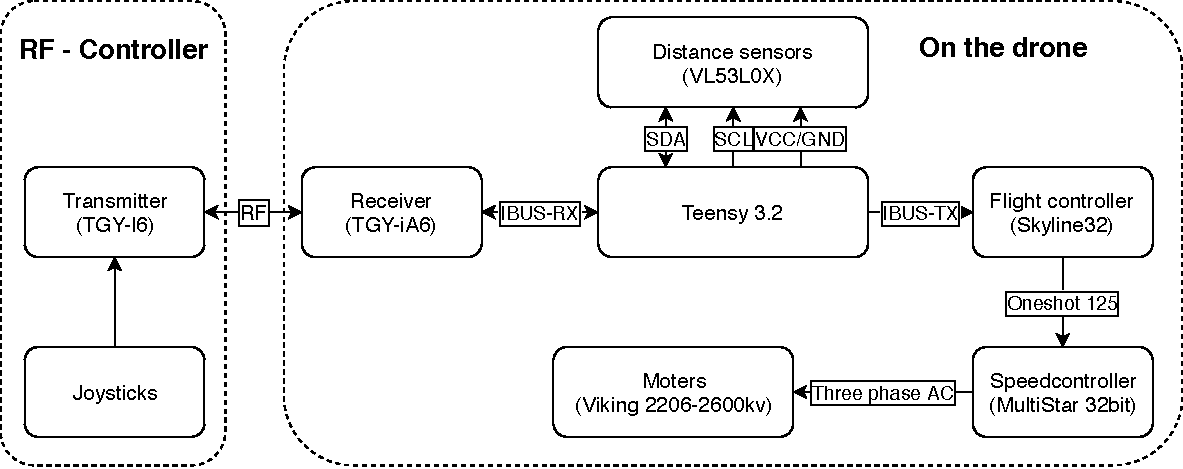
\includegraphics[width=\textwidth]{figures/ch_design/Block-diagram.pdf}
    \caption{Block diagram of how the drone works with the sensors.}
    \label{fig:block_diagram}
\end{figure}

The control diagram consists of a controller part and a drone part. As it can be seen on the system on figure \ref{fig:block_diagram}, the drone will be controlled by a RF controller using a transmitter. The transmitter communicates with the receiver on the drone by RF communication. The desired position received by the receiver will be compared with the measured data from the distance sensors. If necessary the output will be adjusted first or it will be sent to the flight controller directly. This entirely process in drone part is handled by an Teensy 3.2. The flight controller then controls the motor speed, by requesting the desired speed from the ESCs. The different blocks and communications will be described in detail in the following chapters. 
\chapter{Sensor implementation}\label{ch:sensor}
    In this chapter the sensors for the drone will be chosen, so they will fulfill the requirements given for the sensors which can be seen on table \ref{tab:req}.
\section{Time of Flight sensors}\label{s:sensor_choice}
A Time of Flight (ToF) sensor works by sending out a signal, and timing the delay before the reflection of this signal is received. In the section \ref{s:navi} (Navigation) the different types of ToF sensors have been examined, and in that section it have been chosen that the sensor that suit this project most will be ether a IR sensor or a ultrasonic sensor. From these types, the sensor VL53L0X have been chosen, since it fulfill the requirements for this project.

\section{Setup of the sensor}\label{setup_sensor}
Before setting up the sensor to the drone, some technical information is needed to obtain knowledge of these sensors.
First a sketch of the of the sensor is shown in figure \ref{fig:sensor_geometric}, here is both for the transmitting laser and the receiving photo-diode. The Field of Vision from the laser and the photo-diode are the field the sensor can transmit to and receive from. The small field of vision is the receiver and the big one is the transmitter. 
As mention before, the sensor works by sending out a IR signal and times the time used before it receives the reflected signal again.
\begin{figure}[H]
    \centering
    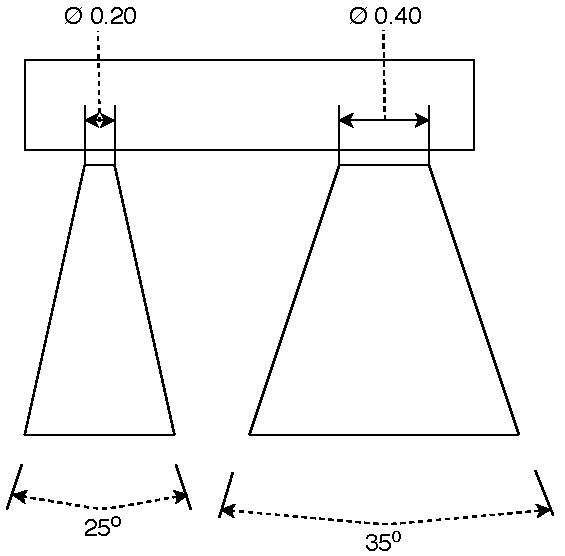
\includegraphics[width=0.6\textwidth]{figures/ch_design/Sensor.pdf}
    \caption{The sensors construction and visual field.}
    \label{fig:sensor_geometric}
\end{figure}
The sensors communicate with a micro controller using i2C, which means it use the pipelines SCL and SDA. The sensors have different modes it works in default mode, high accuracy, long range and high speed. The four modes can be seen in the tabular \ref{tab:sensor_mode}, here both the refresh time and maximum distance for each mode are noted. 
\begin{table}[H]
\caption{Sensor modes.}\label{tab:sensor_mode}
\centering
\begin{tabular}{|l|l|l|}
\hline
\textbf{Mode}          & \textbf{Refresh time} & \textbf{Maximum distance} \\ \hline
Default mode  & 30 ms        & 1.2 m            \\ \hline
High accuracy & 200 ms       & 1.2 m            \\ \hline
Long range    & 33 ms        & 2 m              \\ \hline
High speed    & 20 ms        & 1.2 m            \\ \hline
\end{tabular}
\end{table}
The most suited mode for this project will be the high speed mode, by using this mode the refresh time is faster than the required frequency at 40 Hz.  

\section{Test of sensors}
To see if the VL53L0X sensors are complying ti the requirements from the chapter \ref{ch:Req}. A test have been preformed to determine if the they meet the requirements . The full test of the sensors can be seen in appendix \ref{ap:testOfSensors}. The requirements that the sensors have been tested against are the following:
\begin{itemize}
    \item Detect a surface from minimum 1 meter.
    \item Accuracy of $\pm$5 \% at 400 mm.
    \item sampling rate of 40 Hz
    \item detection of wall with a angle of 0$\degree$ $\pm 10 \degree$
\end{itemize}
The test have been preformed with the sensors mounted on an Arduino with a breakout board faced against a white wall. The code used to test can be found on the Github repository \url{https://github.com/AAU-EIT5/VL53L0X-sensor-test}. 
\newline
\newline
The results of the test can be seen in the figures \ref{fig:des_Sensor1TestResult} and \ref{fig:des_Sensor2TestResult}.
\begin{figure}[H]
    \centering
    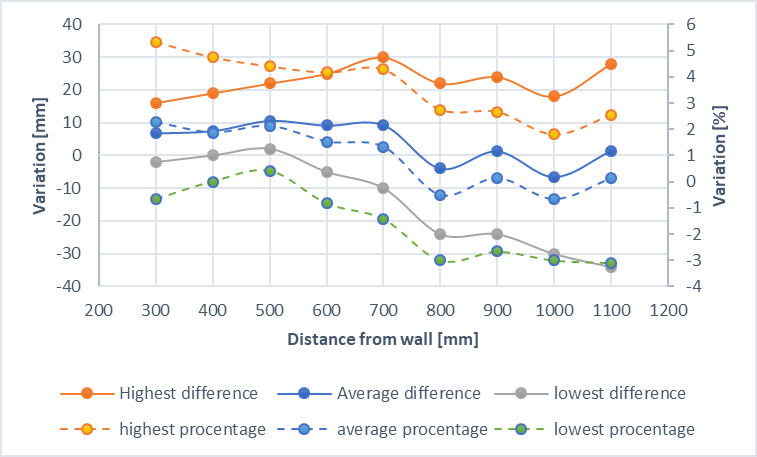
\includegraphics[width=0.8\textwidth]{figures/Appendix/resultatSensor1Test.png}
    \caption{Result of sensor 1 for the test.}
    \label{fig:des_Sensor1TestResult}
\end{figure}
\begin{figure}[H]
    \centering
    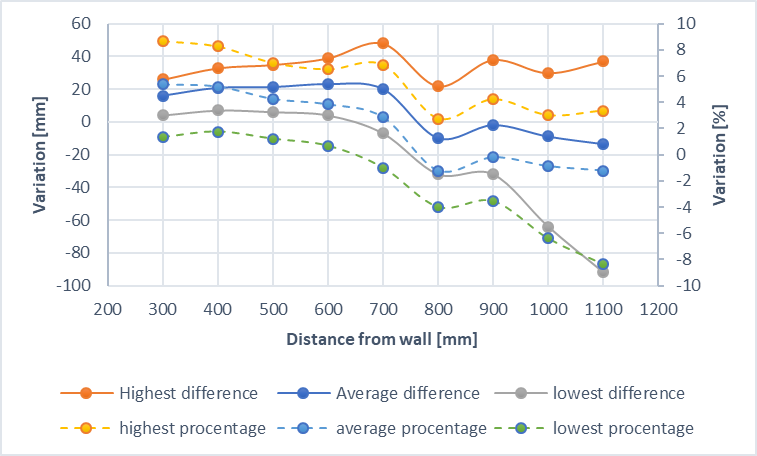
\includegraphics[width=0.8\textwidth]{figures/Appendix/resultatSensor2Test.png}
    \caption{Result of sensor 2 for the test.}
    \label{fig:des_Sensor2TestResult}
\end{figure}
From these results the first requirement of detection of a surface at lest 1 meter can be confirmed. As it can be seen on figure \ref{fig:des_Sensor1TestResult} and \ref{fig:des_Sensor2TestResult}, that both sensors can detected a surface at a distance of at lest 1.1 meter.
\newline
From the figures the second requirement of $\pm5 \%$ accuracy at 400 mm distance can also be confirmed. as it can be seen on the figures the lowest accuracy of the sensors around $\pm 4 \%$ at 400 mm, if the displacement of the sensors measured distance from the real into consideration. As the accuracy are within the requirements, the requirement can be seen as fulfilled.
\newline
As the test was running, a timer was started to measure how long time it takes to complied one set of data, and a sampling rate can be found from these times. The found sampling rate of the sensors are 54 Hz, as the required sampling rate have to be at lest 40 Hz the requirement are meet.
\newline
To test the last requirement, which is to detect a surface at a angle of  $\pm 10 \degree$. This test has performed by placing the sensors 1100 mm from the wall and see if it could detect the wall. The angle is set to $10 \degree$ both for the right and left direction. The result of the test shows that the sensor still is possible to detect a wall. From this test it is therefor conclude that the sensors fulfill the requirements for the sensors.

%
%
%
\section{Interfacing with the sensors}\label{sec:interfacingVL53L0X}%find en bedre overskrift
For interfacing with the VL53L0X the library VL53L0X from Polulu will be used.
\newline
To start, the address of the sensor have to be setup, this are done by the \textbf{\textit{setaddress()}} function. After setting the address, the sensors is initialized with the function \textbf{\textit{init()}}. To change the time the sensors have to measure the distance, the function \textbf{\textit{setMeasurementTimingBudget()}}, where the  \textbf{\textit{budget{\_}us}} are the time in microseconds.
To start the measuring continuously the function \textbf{\textit{startContinuous()}} is used, and with this the setup of the sensors is done.
To get a measuring in continuous mode the function \textbf{\textit{readRangeContinuousMillimeters()}} is used.

%As mentioned earlier in section \ref{setup_sensor} the VL53L0X sensors uses i2C at the communication method 
% her skal der stå hvordan sensorne settes op så værdier kan læses.
    


\begin{comment}
\section{Test of Laser ToF sensors}
In order to test the chosen sensors, a test system has to be built.
We decided to use an Arduino Uno, with a custom made breakout board, to interface the two VL53l0X sensors to the arduino.

The two VL53L0X sensors communicate over i2C (Inter-Integrated Circuit) which is a 2-wire bus, with one master and up to 127 slaves, as each slave has a 7bit address. The VL53L0X starts up on a fixed address, but can have a custom address configured. By making use of the shutdown pin on the sensor, one can sequentially turn on the sensors, give them a new address and then continue to the next sensor.

We have decided to use the Pololu Arduino library\cite{vl53l0x_lib} for the VL53L0X sensors, as it implements the required modes, as well as setting new addresses.
\end{comment}

\chapter{Interfacing with the drone}\label{ch:drone_interfacing}
    \section{Communications}\label{s:coms}
In order to control the drone, there has to be a way to transmit commands to the drone. This can be anything from simple commands like "arm motors" or complicated commands like streaming movement commands to the flight-controller on the drone.
This section will go over a few different physical layers, and will then go in detail with.

\subsection*{Proprietary TX RX pair}\label{ss:rc-txrx}
One very common solution for radio controlled devices to communicate, is over a proprietary RF link. These systems have a remote control as the transmitter (TX) that the operator use to control the drone, and the drone then has a receiver (RX) that outputs command to the drones flight-controller.
\newline
In order to modify this signal, there are few places to break in to the signal and modify it. One could rewrite the firmware for the flight-controller, but this is out of scope for our project. This only leaves options that tap into the signal, modify it, and send the modified signal to the drone.
This can either be done in the RF signal, in the controller hardware, or between the RX and flight-controller. 

We have chosen to tap in between the RX and flight-controller, as this is the only place to tap in, that's standardized, and this following sections will detail the protocols used here.\\
\newline

\subsection*{Drones radio frequency specification}
In this section the RF speficaition for drone will be examined. 

\begin{table}[H] \label{tab:RFSpec}
\begin{tabular}{|l|c|}
\hline
\multicolumn{2}{|c|}{\textbf{RF Specifications for communication between controller and the drone}}                               \\ \hline
RF range           & 2.405 - 2.475 GHz                                         \\ \hline
Channel bandwidth  & 500 KHz                                                   \\ \hline
Number of channels & 142                                                       \\ \hline
RF power           & Less than 20 dBm                                          \\ \hline
RF mode            & AFHDS 2A (Automatic frequency hopping digital systems 2A) \\ \hline
Modulation type    & GFSK                                                      \\ \hline
Antenna length     & 26 mm * 2 (dual antenna)                                  \\ \hline
RX sensitivity     & -105 dBm                                                  \\ \hline
\end{tabular}
\end{table}
The RF specification in table \ref{tab:RFSpec} system works within 2.405 to 2.475 GHz. There is 142 channels and each have 500 KHz bandwidth. For each transmitter there is unique ID, when the transmitter is connected to the receiver, the receiver will save the transmitters ID, and this way the receiver will avoid other transmitter signal.
AFHDS2A, which stands for Automatic frequency hopping digital system 2A is used for radio frequency mode. This means AFHDS2A has the automatic identification function, which switches automatically in current mode between single-way communication mode and two-way communication mode. The AFHDS2A have multiple and error-correction built it, this improves the stability of the communication and reduces the error ratio and extend the reliable transmission distance. The drones transmitter and receiver can be found in datasheet.










\subsection*{RX protocols}\label{ss:rxprotococls} 
The RX connects to the flight-controller, using one or more channels where each channel carries a control signal for a function on the drone. These channels can either be transmitted over one wire each, using PWM to express the value of the channel, or they can all be transmitted over one wire, using PPM or other serial protocols to express the value of each channel.\\

\begin{figure}[h]
    \centering
    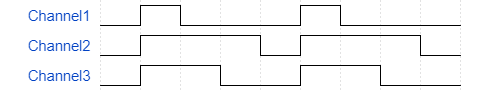
\includegraphics[width=0.8\columnwidth]{figures/PA/pwm.png}
    \caption{3 Channels sent over PWM, sending the values 25\%, 75\%, and 50\%}
    \label{fig:chan_pwm}
\end{figure}

\begin{figure}[h]
    \centering
    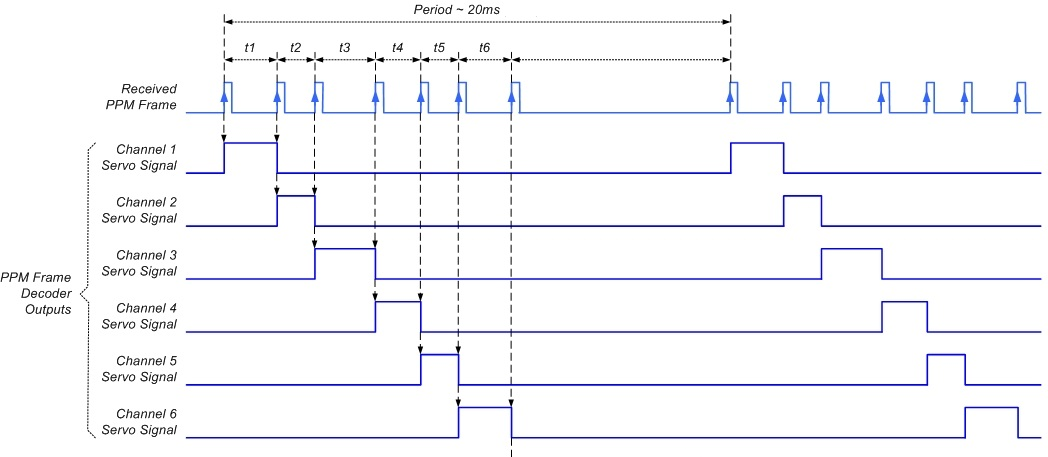
\includegraphics[width=0.8\columnwidth]{figures/PA/post-229-0-40047400-1404173046.jpg}
    \caption{3 Channels sent over PPM, sending the values 25\%, 75\%, and 50\%}
    \label{fig:chan_ppm}
\end{figure}
  %\todo{Redo figure for PPM, I have no source for the current one.}
  
With PPM, values are sent sequentially. Before the first channel is sent, a long "End of frame" pause is sent, holding the data-line low. This ends with a pulse, signifying start of channel1 value. Some time later, a second pulse signifies end of channel1 value, and start of channel2 value. This pattern continues until all channels have been sent, after which the "End of frame" pause is sent again.

A common problem with PWM and PPM based transmission of channel values, is that these methods encode the channel values as time between pulses of one sort or another, this means they are susceptible to jitter in the clocks on both the transmitting and receiving system.\\
In order to solve this, other serial protocols can be considered.
One such serial protocol is used internally in the receiver used on our drone. The protocol is called flySky iBUS, and is a variation of the very common RS232 serial protocol. The data-rate is fixed at 115200 baud, with 8 data bits, and 1 stop bit, or 8N1.

\begin{figure}[h]
    \centering
    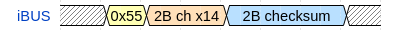
\includegraphics[width=0.8\columnwidth]{figures/ch_design/iBUS.png}
    \caption{A single iBUS packet}
    \label{fig:iBUS}
\end{figure}

As shown on figure \ref{fig:iBUS} an iBUS packet consists of a header-byte then 28 bytes, carrying 14 16-bit values, followed by a simple 2B checksum. The checksum is a sum of all 14 values transmitted.

Due to the benefits that iBUS caries over PWM and PPM, this is the protocol we have decided to further use in our project.

\subsection*{iBUS decoding and encoding}\label{iBUS library}

The code developed to decode and encode iBUS is available on our github\cite{ibus-lib}.
It was written as a generic Arduino library, and this section will document key functions from it.

\begin{lstlisting}[language=C++, caption={Parser for iBUS packets}]
void iBus::m_parse_channels(uint8_t packet[], int ch[])
{
	// For each channel, store 2 bytes in 16bit integer
	// The values are sent MSb first, LSB first
	for(int i=0; i<m_channels_per_packet; i++)
	{
		ch[i] = packet[i*2+2] << 8 | packet[i*2+1];
	}
}
\end{lstlisting}

This function loops over all channel bytes in an iBUS packet, and combines them into integers in internal array to the library, a simple getter is them provided for the main program, to get individual channels.

The reverse is done to build a packet for transmitting, as seen in the following function

\begin{lstlisting}[language=C++, caption={Function for constructing and transmitting for iBUS packets}]
void iBus::m_send_packet(int ch[])
{
	// Set up buffer and set header byte
	uint8_t buff[m_packet_size];
	buff[0] = 0x55;

	// For each channel, unpack 16 bit integer into bytes
	// The values are sent MSb first, LSB first.
	for(int i=0; i<m_channels_per_packet; i++)
	{
		buff[i*2+1] = (ch[i] & 0x00FF);
		buff[i*2+2] = (ch[i] >> 8);
	}
	int checksum = m_get_checksum(ch);

	buff[29] = (checksum & 0x00FF);
	buff[30] = (checksum >> 8);

	m_ser.write(buff, m_packet_size);
}
\end{lstlisting}

As seen in this function, constructing and sending an iBUS package is rather simple. the code allocates a buffer to hold a packet, sets the header-byte, and then splits apart the 14 channels supplied into individual bytes, arranged MSb, LSB first. this means a number such as 0x0102 would be sent as 0x02, 0x01.From here, the checksum is calculated, split into the same MSb, LSB first arrangement, and the whole buffer is written out over the allocated stream object m\_ser.

The function used to set which channel values are sent, is a simple setter function, setting the values of an internal out-put channel array, which is passed to m\_send\_packet\(\) each time the main ticker function handle\(\) is called.

the handle function is more easily described with a flow-chart, as it is a relatively long function, but it's tasks are fairly simple.

\begin{figure}[h]
    \centering
    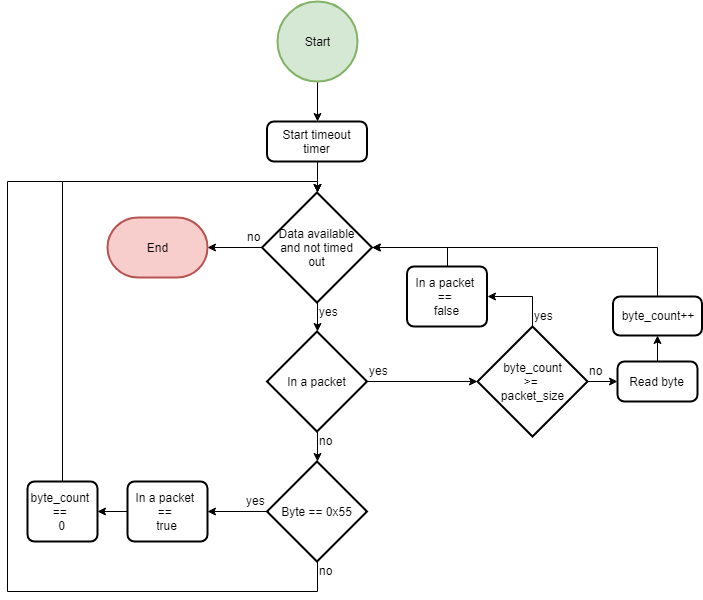
\includegraphics[width=0.8\columnwidth]{figures/ch_design/ibus-handle-flowchart.png}
    \caption{Flowchart descriping the handle function in the iBUS library}
    \label{fig:ibus_handle_flowchart}
\end{figure}


\chapter{Model of the drone}\label{ch:model_drone}
    %\section{Drone movement}\label{s:drone_movement}
In order to make a transfer function for the drone it is needed to examine how the drone behaves when it moves around. To make it simple the drone is set to only move in z-axis also known as yaw axis \ref{fig:z_axis}.
\begin{figure}[H]
    \centering
    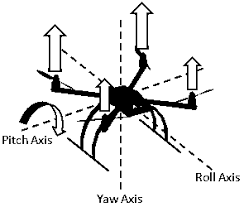
\includegraphics[width=0.45\textwidth]{figures/ch_movement/z-axis.png}
    \caption{Illustration of \cite{drone_axis}}
    \label{fig:z_axis}
\end{figure}


 As mentioned in the requirement specification \ref{sec:req}, the drone should keep a fixed distance to the floor. To be able to control the drone in the z-axis, a model for the drone will be determined. This model describing how the drone corresponds to controller inputs. The position on the z-axis is controlled by the throttle on the remote controller. The throttle values is set from 1000\% - 2000\%, where the drone is idle at 1000\% and maximum velocity at 2000\%.  

\section{Vicon}
To determine the behaviour of the drone, it is important to know how the the drone response to the remote controller. 
Because the models are of a drone, driven by a flight controller with an unknown control system, it seems inaccessible to derive the models analytically. Instead, by measuring either an impulse response or a step
response in the z axis, the models can be determined experimentally. For this a motion tracker system, for tracking the positions of the drone. A motion tracker system called vicon is available at the university laboratory. 

\section{Transfer function for the movements}\label{s:transfer_function}
To get a model of the drone, it is needed to get a transfer function for the drones movements. To get the transfer function, a model of the drone's movements is needed, to get these data the system Vicon is used. The data that is needed is for a step response, this step response will only be for the z-axis. When this step response is plotted it gives a function, this function will be use to make the transfer function. This function is called h(s)
that depends on the input and output of the function. All these functions depends on the time. To get a better view of have this transfer function works can be seen on the figure \ref{fig:transfer_function}.
\begin{figure}[H]
    \centering
    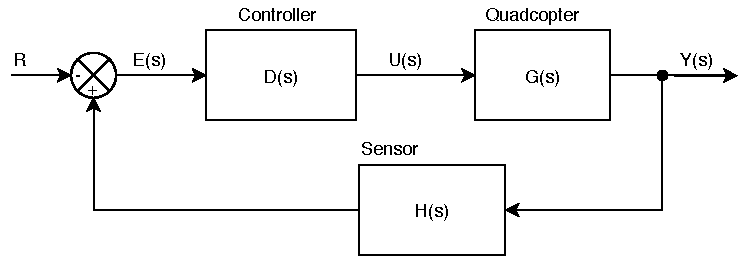
\includegraphics[width=0.75\textwidth]{figures/ch_design/transfer_function.pdf}
    \caption{An illustration of the transfer diagram}
    \label{fig:transfer_function}
\end{figure}

From this diagram it can be seen that the transfer function is applied an unit step $\frac{1}{s}$. 







\chapter{Design of controller}\label{ch:design_control_sys}
     \begin{figure}[H]
     \centering
     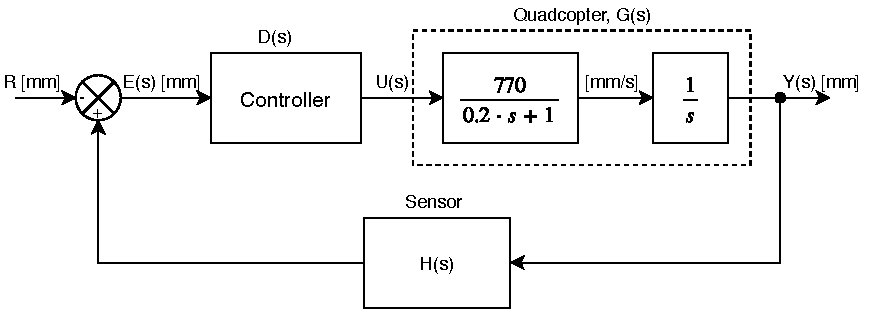
\includegraphics[width=\textwidth]{figures/ch_design/controller/ControlDiagramTF.pdf}
     \caption{Block diagram illustration of the control system  to control the levitation of the Quadcopter.}
     \label{fig:controlDiagram}
 \end{figure}

%To avoid steady state error, it is necessary to examine PID controller, which stands for proportional integrate derivative controller.
To make the full control loop, there are needed two more components apart from the transfer function. This can be seen in figure \ref{fig:controlDiagram}. From this figure it is visual that there is needed a function for the sensors and a controller of the control loop. 
First the function for the sensor will be found and afterward the PID controller will be examined with all the components.


\section{Feedback control loop}\label{s:feedback_loop}
To design a control system, a feedback control loop is needed. Normally it will just be a factor like 1, but in this situation, the feedback in the control loop, will be the feedback from the distance sensors. To get an expression for the feedback, a equation is used. Because the feedback is coming from a sensor, that need to sample the data needed to the feedback, the expression in equation \ref{eq:formular_sampling_feedback} is used \cite{digital_control}.
\begin{equation}\label{eq:formular_sampling_feedback}
    H(s)=\frac{2/T}{s+2/T}
\end{equation}
In this equation the T is the sampling time for the sensor, in this case the sampling time is $25\ ms$, so the expression for the feedback loop will be as seen in equation \ref{eq:feedback_loop}\cite{feedback_control}.
\begin{equation}\label{eq:feedback_loop}
    H(s)=\frac{\frac{2}{0.0025}}{s+\frac{2}{0.0025}}
\end{equation}

\section{PID controller}
To figure out what kind of controller there are needed in the system, to get the right output of the system. In this case the PID controller of a first order close loop system will be explained to find the best suited controller for the system. In the PID controller, there are both a proportional part, an integral part and a derivative part. All these three parts have influence on the output signal. 

\begin{figure}[H]
    \centering
    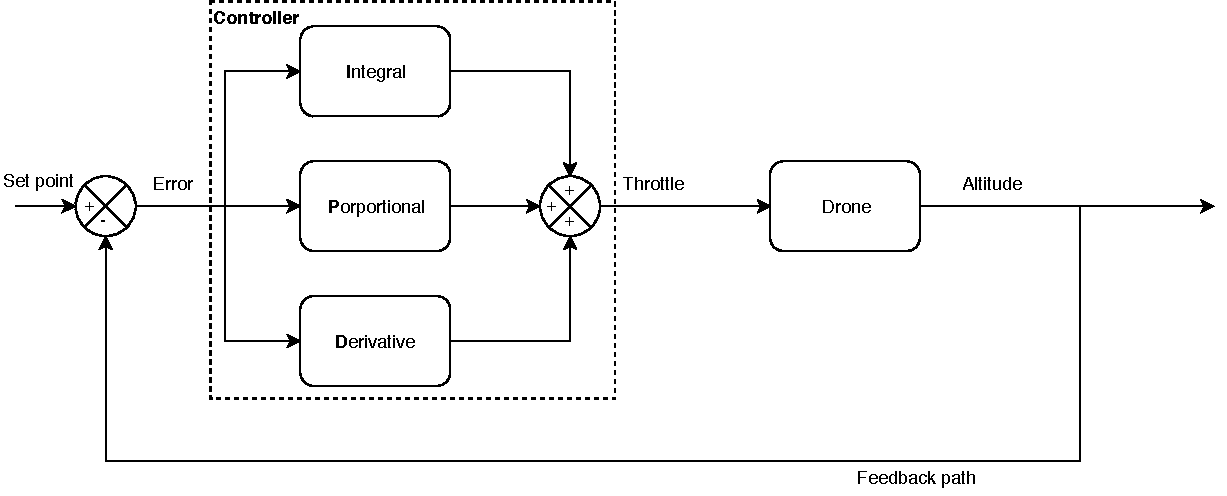
\includegraphics[width=0.9\textwidth]{figures/ch_design/PIDController/PIDControl.pdf}
    \caption{Illustration of a PID controller connected in a control loop.}
    \label{fig:PID_Controller}
\end{figure}
As shown in figure \ref{fig:PID_Controller} the focus for this control system, will be on a closed loop control system. This is used because of the implementation of the sensors in the system. To control this system a PID controller will be used, or a part of it. First the different parts of the PID controller will be explained. The three parts that will be explained are the proportional part, the integral part and the derivative part \cite{digital_control}.

\subsection*{Proportional controller}
The proportional control is in most cases the main driving force in a controller. The proportional control changes its output in proportional to the error. 
The function for the proportional correction, is shown in equation \ref{eq:kp}.
\begin{equation}\label{eq:kp}
    \frac{U(s)}{E(s)}=K_p
\end{equation}
In equation \ref{eq:kp}, the E(s) function is the error on the input and U(s) is the output after the controller part as seen on figure \ref{fig:controlDiagram}.
If the $K_p$ gets increased, a larger error can be corrected, but in situations the $K_p$ value gets too big, the error will get larger too. The proportional controller can only correct constant error on the gain. By choosing a very small $K_p$ value the error is big, and by choosing $K_p=1$ there will be corrected no error. If a too big $K_p$ value is chosen will the control loop begin to oscillate and eventually become unstable. If the $K_p$ is too low, the control loop will not respond enough to disturbances or set point changes. The proportional controller is used for set the phase margin and gain margin to the optimal setting \cite{digital_control}. 


\begin{comment}


The following graph \ref{fig:P_Control} will illustrate a proportional control, and what will happen, when a drone rises to a giving altitude, which in this case it will be 40 cm. 
\begin{figure}[H]
    \centering
    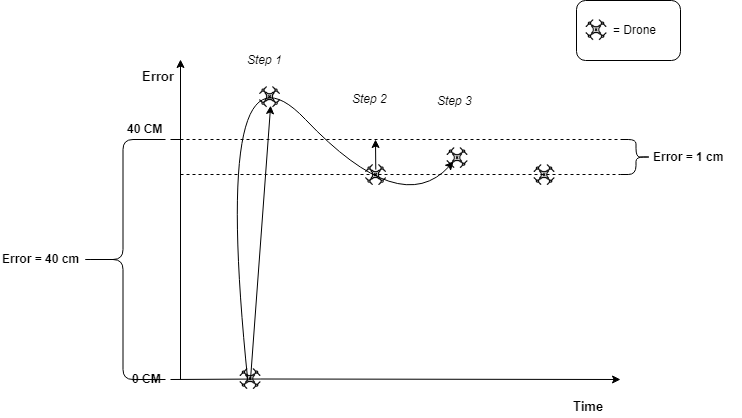
\includegraphics[width=0.8\textwidth]{figures/ch_design/PIDController/ProportionalGraph.png}
    \caption{Illustration of a proportion control system.}
    \label{fig:P_Control}
    \end{figure}
The graph \ref{fig:P_Control} at the starting point there is an error of 40 cm, since there is large of error, it will generate a large propeller speed, which the drone will rise. In step 1 at 40 cm, the error is equal 0, and at this point the propeller speed decrease and the drone will fall back to earth. However, since the propeller speed is large, it will have overshoot as seen in the graph (step 1). When it is under 40 cm the propeller speed will increase again and since the error is 1 and is not large, it will increase the propeller speed slightly as seen at graph (step 2). To hover the drone, its need a certain propeller speed, where the lifting force is exactly equal to the weight of the drone, that speed will hover the drone.    

To hover the drone at certain altitude will depend on the controller gain and propellers speed. In this example we assume that at 80 rpm the drone will hover, if the proportional gain is 2 and the drone is at starting point, which the error is 40 cm, the drone would hover right at the ground level since 2 \(\times\) 40 is 80 rpm. The following graph \ref{gra:P_Control_graph} illustrates where the drone will hover, when the gain increases.

\begin{figure}[H]
    \centering
    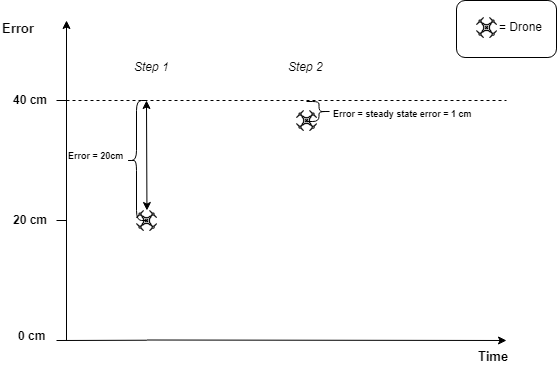
\includegraphics[width=0.6\textwidth]{figures/ch_design/PIDController/ProportionalGraph1.png}
    \caption{Proportional control graph.}
    \label{gra:P_Control_graph}
    \end{figure}
The graph \ref{gra:P_Control_graph} at step one the proportional gain is set to 4, which the error is reduced to 20 cm, since the drone is closer to the set point. In step two the proportional gain is 80 and the drone is hovering at 39 cm, which the error is 1 cm. This constant error is also called steady state error and this will never be eliminated in proportional control. There is a need of a or control mode, which can use past information to eliminate the steady state error. 

\end{comment}

\subsection*{Integral controller}
Apart from the proportional controller, an integral controller always works on the changing error, to make the error goes to zero. The ways this controller works on is by continuously increment and decrements the controller's output to reduce the error from the loop. 

The error correcting time can depend on the sixe of the error. The time used is defined be the size of $T_I$ in the equation, can also be seen in equation \ref{eq:integral_control} \cite{digital_control}. 

\begin{equation}\label{eq:integral_control}
    \frac{U(s)}{E(s)}=\frac{k_I}{s} \to u(t)=k_I \int_{t_0}^t e(\tau) \ d\tau
\end{equation}
In this equation $k_I$ is th integral constant. It can be seen from the equation, that the size of $k_I$ has influence on the reaction time. If this value is small the reaction time will be fast, but if it is a big value it will have the opposite effection. If the time is set to small the control part can be slow, but if the time is set to big the control loop can begin to oscillate and become unstable. The upside of using a integral controller, is to add more gain for the transfer function. By doing this the steady-state behavior will be improved along side the adding of gain. 
If the $k_I$ get to big it can also increase the overshoot for the control loop\cite{digital_control}. 


\subsection*{Derivative controller}
The derivative controller is mostly used in a motion controller. There are some problem related to this type of controller, it is very sensitive to measurement noise and it makes it difficult to make trial-and-error tuning.  It still make the response faster then by using a PI-controller only \cite{digital_control}. 

The way the derivative controller works is by producing the output on the rate of changes of the errors. By doing this the derivative control, can be said to work on the errors, by correcting them by look on the past. This means the controller correct errors at a high rate, and if there are no errors the derivative controller will be zero. The equation for the derivation controller can be seen in equation \ref{eq:derivative_control} \cite{digital_control}.

\begin{equation}\label{eq:derivative_control}
\frac{U(s)}{E(s)}=k_D \cdot s
\end{equation}

In this equation the $k_D$ is the derivative time. The larger the derivative time is set to, the more higher the action form the controller will be, but if the time is set to high the controller will begin to oscillate and become unstable. And if the derivative time is to small the influence on the output will be slower \cite{digital_control}. By implementing a derivative controller, increase the phase. By increasing the phase, the phase margin also improves and thereby the damping of the transfer function.

\section{Differences between the PID-controllers parts}\label{s:different_pid}
To compare the different combination between the PID-controller's parts, first a bode plot of all the components will be made to compare how they infect the bode plot. This bode plot can be seen figure \ref{fig:PID_bode}.

\begin{figure}[H]
    \centering
    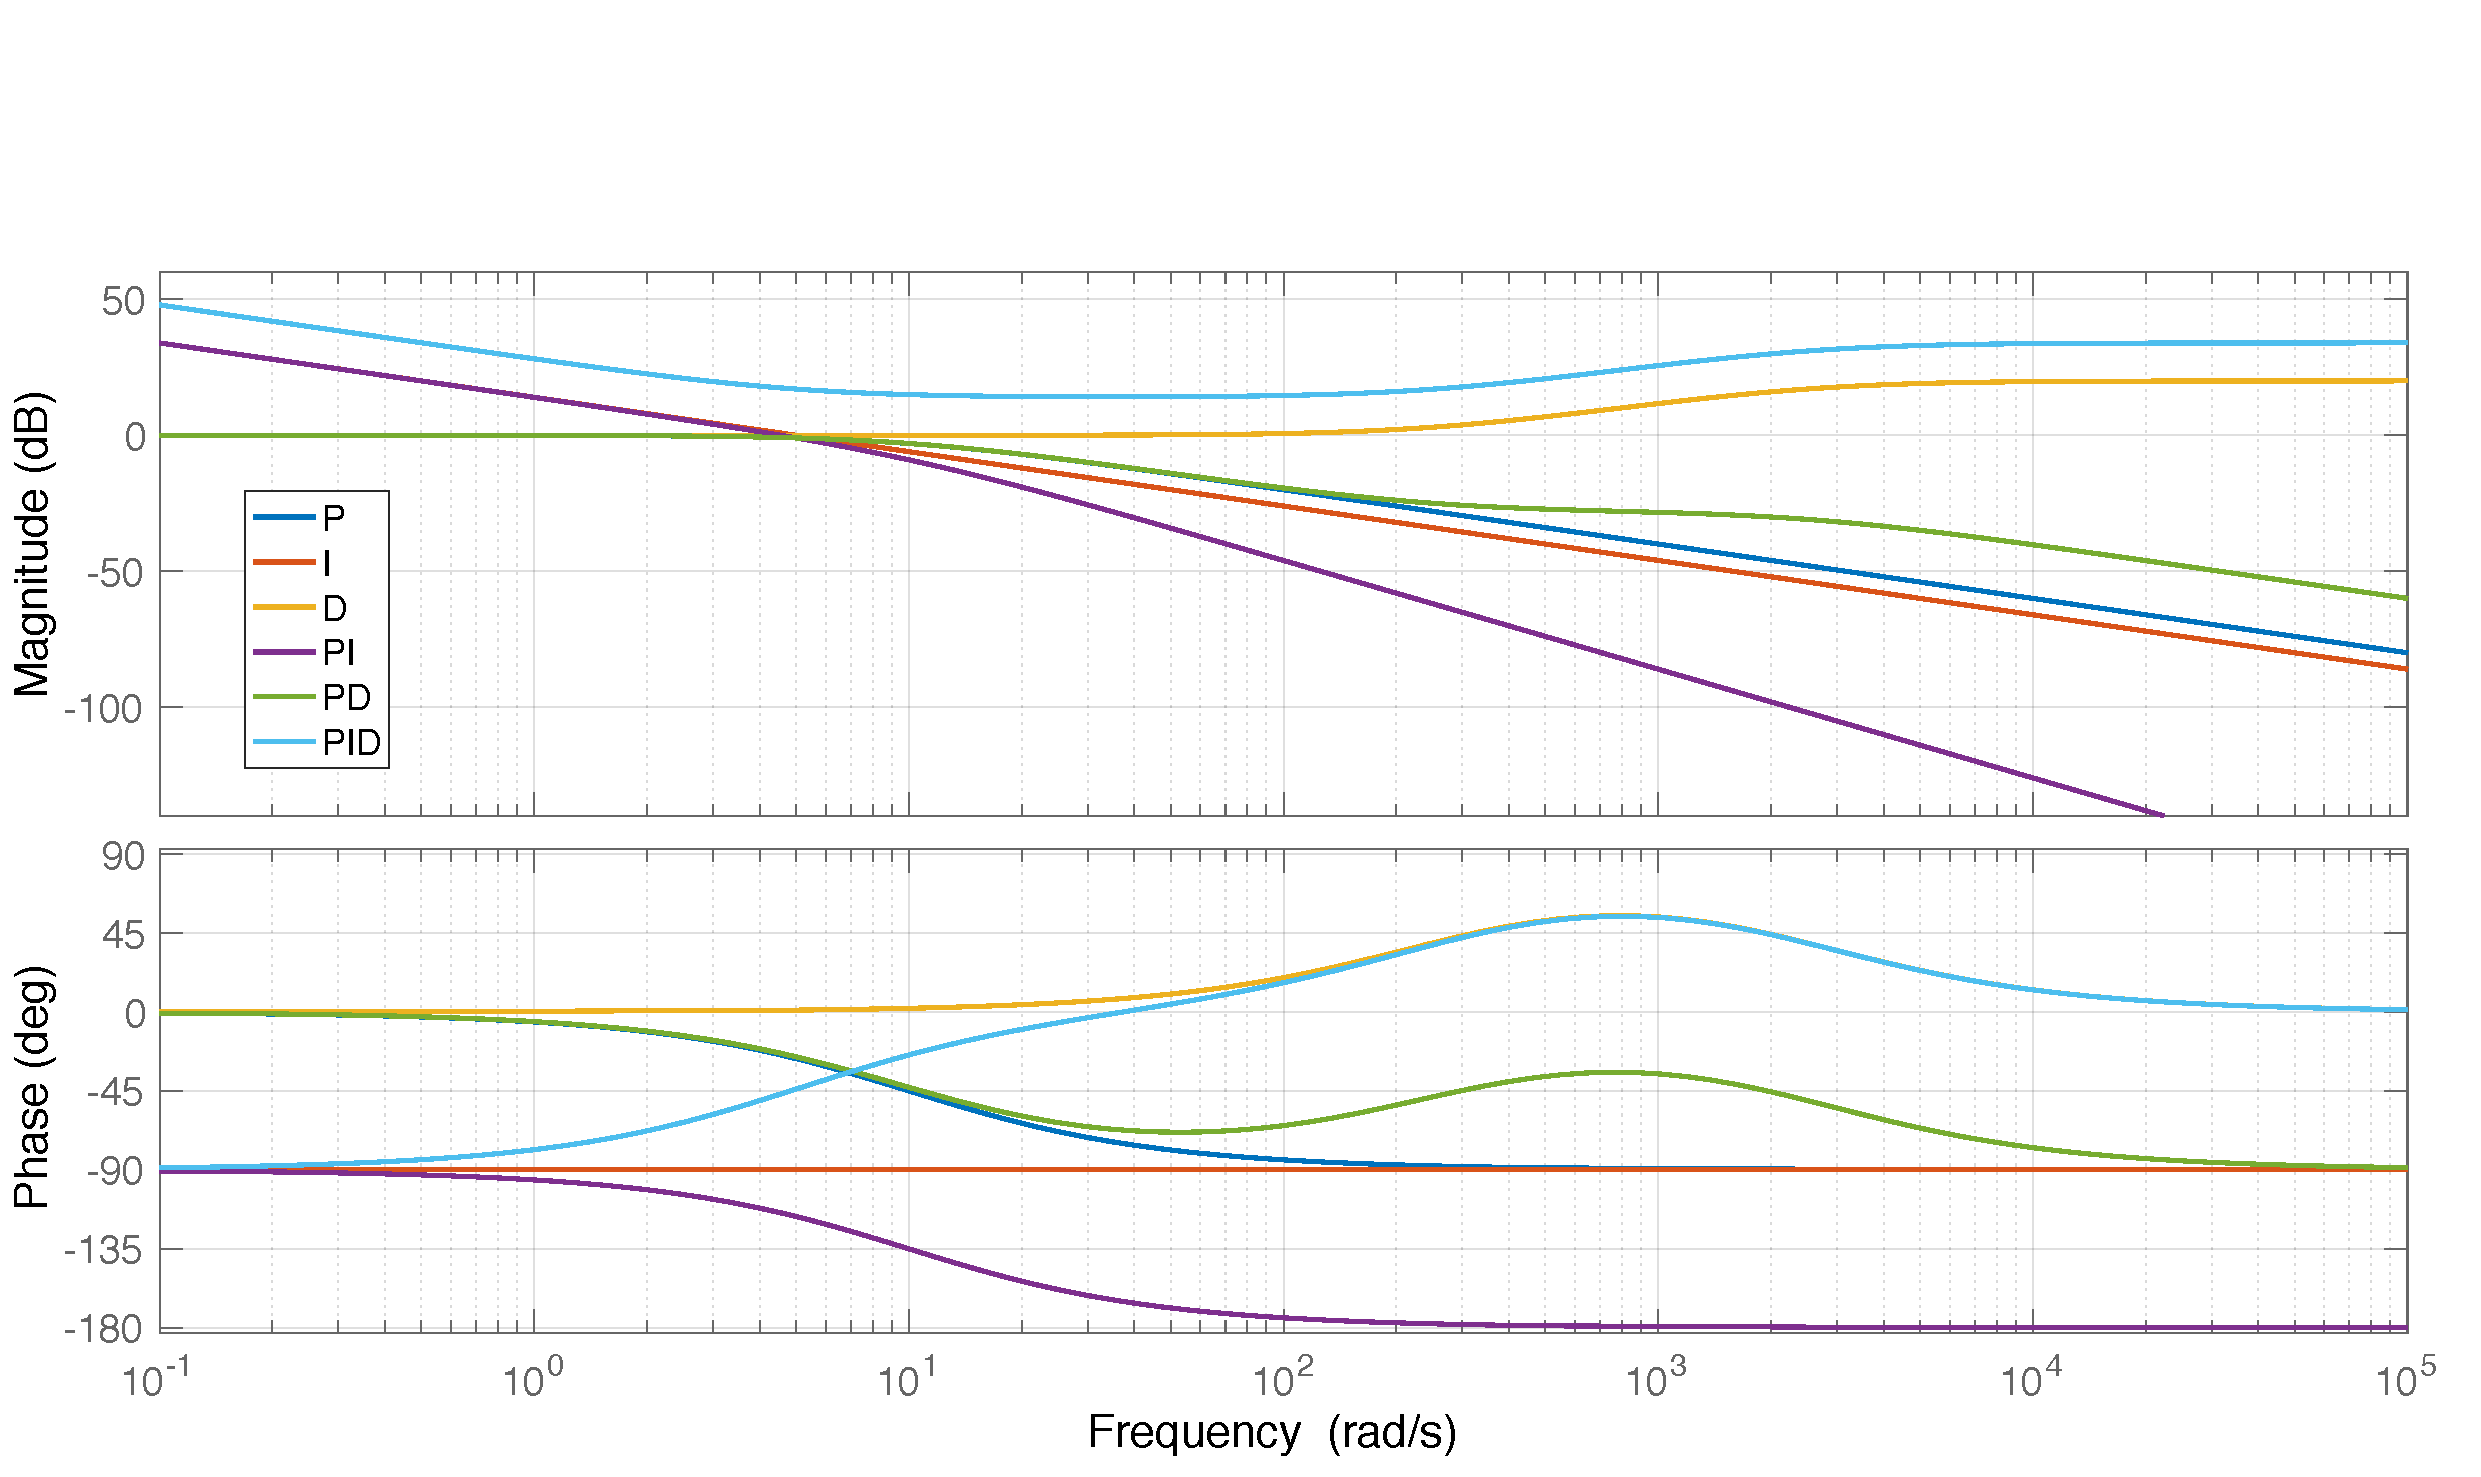
\includegraphics[width=\textwidth]{figures/ch_design/controller/Bodeplot_PID.pdf}
    \caption{An example of the different bode plot for the different PID-control part, to illustrate how they work on the gain and phase, both individual and combine with another.}
    \label{fig:PID_bode}
\end{figure}
From this figure it can be seen how the gain and phase is affected by the changes in the $K_p$, $k_I$ and $k_D$. It is also visible to see that the integral controller affects the gain but not the phase, only when it is combined with the proportional controller. 
It can also be seen that the derivative controller change the phase but not the gain as much. All these combinations can be used in different ways, but first for this project a proportional controller will be calculated, this will be done in the next section.

% http://blog.opticontrols.com/archives/344
\section{Design of proportional controller}\label{sec:design_controller}
As it has been decided to use a proportional controller to regulate the system, the proportional gain $K_p$ has to be found. 
When finding the value of $K_p$ the requirements from chapter \ref{ch:Req} have to be taken into consideration. 
The requirements that have to be taken into consideration are:
\begin{itemize}
    \item Overshoot of max 30\%
    \item Settling time of  max 10 seconds
    \item Steady state of $\pm$5\%
\end{itemize}
To find $K_p$ we have to start finding the damping factor. From the allowed overshoot the damping ratio $\zeta$ can be found with the equation \ref{eq:dampingRatio} \cite{nise2007control}.
\begin{equation}\label{eq:dampingRatio}
    \zeta = \frac{-\ln(overshoot/100)}{\sqrt{\pi^2+\ln^2(overshoot/100)}}
\end{equation}
With a overshoot of 30\% the damping ratio are found to be 0.358, and from this ratio the phase margin $\Phi_M$ can then be found with the use of the equation \ref{eq:phaseMargin} \cite{nise2007control}.
\begin{equation}\label{eq:phaseMargin}
    \Phi_M = \arctan\left(\frac{2\zeta}{\sqrt{-2\zeta^2+\sqrt{1+4\zeta^4}}}\right)
\end{equation}
The phase margin is calculated to 0.682 radian which are equal to $39.09\degree$. By making a bode plot of the open loop term ($G(s)H(s)$) from  the diagram in figure \ref{fig:controlDiagram} can the gain adjustment be fund.
In figure \ref{fig:des_bodeplot} can the bode blot of $G(s)H(s)$ be seen, where the gain margin, at the phase margin of $39.09\degree$, can be fund to be 39.7 dB.
\begin{figure}[h]
    \centering
    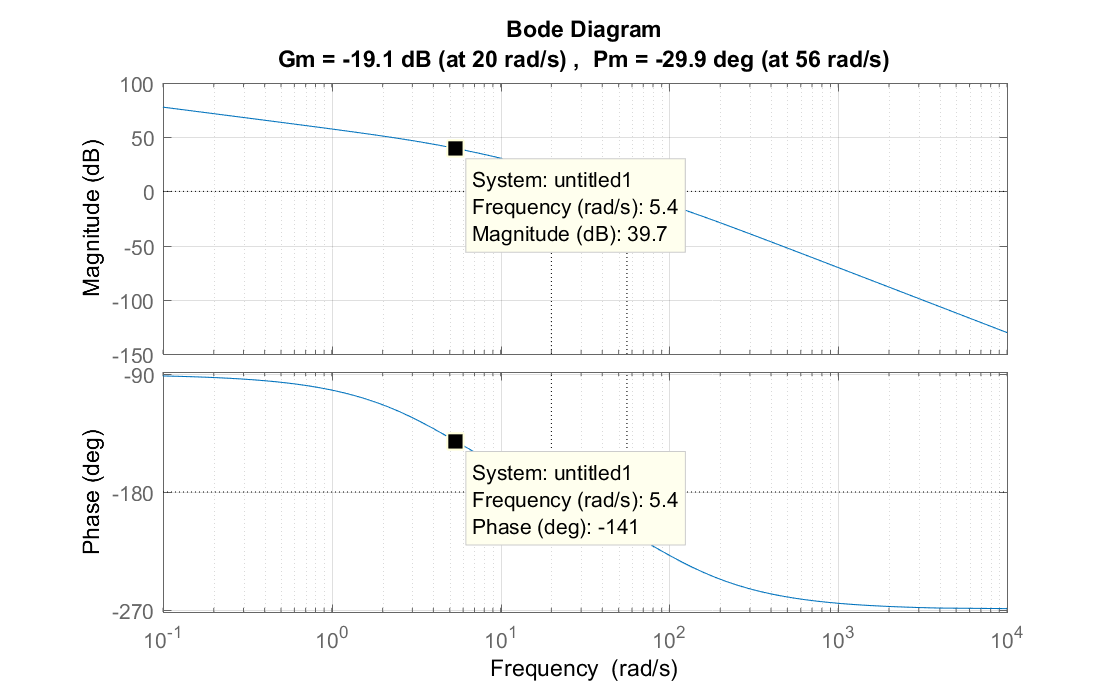
\includegraphics[width=0.8\textwidth]{figures/ch_design/controller/bodeplot.png}
    \caption{Bode plot of the open loop term ($G(s)H(s)$) with the phase margin of 39.09$\degree$ and the corresponding gain margin.} 
    \label{fig:des_bodeplot}
\end{figure}
\newline
To get the value of $K_p$ the magnitude have to be adjusted so the gain margin are 0 dB, this can be done by decreasing the calculated gain margin of 39.7 dB.
The -39.7 dB have to be converted to a gain factor, which have been done by using the following equation \(10^\frac{dB}{10}\) and calculated the factor to 0.01. This mean $K_p$ is 0.01.
With $K_p$ found the control diagram of the system get to be as seen in figure \ref{fig:dec_Final_block_diagram}.

\begin{figure}[H]
    \centering
    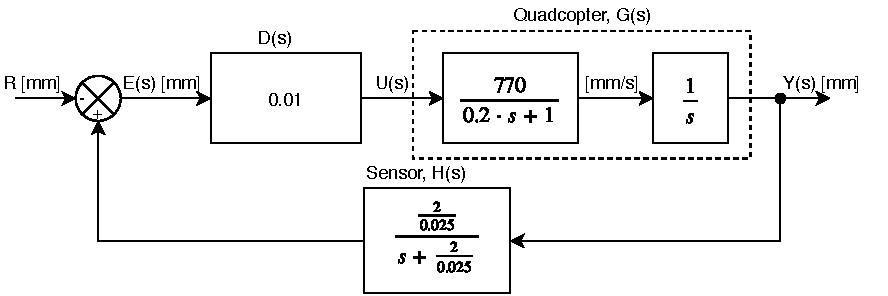
\includegraphics[width=\textwidth]{figures/ch_design/controller/FinalControlDiagram.pdf}
    \caption{Block diagram of the final control system.}
    \label{fig:dec_Final_block_diagram}
\end{figure}







    \section{Simulations}

    \section{controller implementation}\label{sec:control_code}
The controller is implemented digitally, running as code on a micro-controller, this section will describe how the controller has been implemented in the code

\begin{figure}[H]
    \centering
    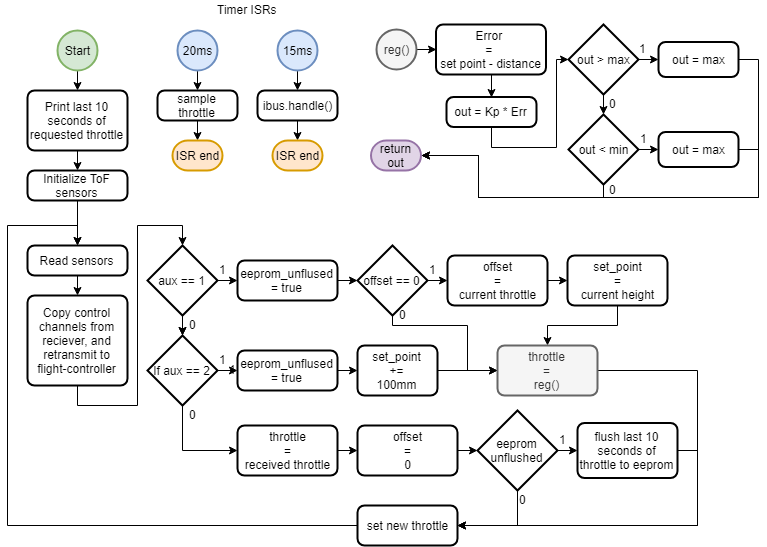
\includegraphics[width=1\textwidth]{figures/ch_design/controller/EIT5-code.png}
    \caption{Flowchart of the code}
    \label{fig:code_flowchart}
\end{figure}

The flow-chart can be broken into 4 major blocks. First is the power-on initialization, which is the first 2 blocks following the green "start". The second logical block would be the two different Interrupt Service Routines or ISRs starting with a blue circle, and ending on an orange bar. Third would be the regulator function, starting with a gray circle, and returning with a purple bar, and the fourth block would be the main program loop, consisting of the entire bottom part of the flow-chart.

\subsection*{Initialization}
This code runs once on start up, and waits 5 seconds for a serial connection to be established on it's USB port. If a serial instance is started, it prints out 1000 samples of the last 10sec of regulated throttle stored in EEPROM as comma separated values.
Then it sets up regularly timed ISRs, one to handle the iBUS communication every 15ms, and one to sample the currently set throttle every 20ms.
The Teensy 3.2 supports prioritized interrupts, and as such, the communication handling has been given a higher priority, as without it, the drone could shut off mid-flight.

\subsection*{ISRs}
The two ISRs are quite different, both in size and execution time.
The smallest is the \textit{"sample throttle"} ISR, which samples the currently set throttle value to a FIFO-buffer of 1000 samples. This is done both to limit EEPROM writes, and to keep it quick.\\

The second ISR runs the handle() function of the iBUS object. This is a larger function that, best case, reads no bytes, and transmits 31 bytes. 
Worst case the function spends 2ms reading incoming serial bytes, then sending a 31 byte iBUS packet.
Most of the time, the function will have 3.75 iBUS-packets waiting in its RX buffer, and have to send 1. If we round this up to 5 31 byte iBUS-packets it has to handle in total and assume that covers overhead, then at 115200 baud, this function will at most, take $5 * 31 * \frac{1E6}{115200} = 1345.5$  $[\mu{}s]$ 
This is fine for an ISR run on the Teensy 3.2

\subsection*{Regulator}
For this project, as discussed in chapter \ref{ch:model_drone}, we've decided to use a proportional regulator. This is implemented in this function, where first the current error is calculated, then this error is multiplied with the gain Kp, and this output value is then constrained to be within two minimum and maximum values before being returned. 

\subsection*{Loop}
This is the constantly looping part of the code, and this consciously reads the sensors, and transparently passes the incoming iBUS packets to the flight-controller on the drone. After that, it checks if the aux channel used for initiating regulation is in one of three states.\\

\textbf{0:}
If it's in state 0, the throttle is read from the incoming iBUS packets, and passed to the drone, allowing for complete manual flight of the drone, additionally this state resets if throttle-offset the drone uses when regulating, and if the drone has been regulating, it flushes the last 10 seconds of throttle values to EEPROM.\\

\textbf{1:}
If it's in state 1, and the offset hasn't been set yet, the drone will save the current throttle as the offset required to hover, and will then set the set-point for regulation, to the current height.
This allows the drone operator to fly the drone to a height where it hovers, before enabling regulation. 
It will then run the regulator, assigning the output to the throttle channel

\textbf{2:}
If it's in state 2, it will run the regulator with a +100mm set-point, compared to state 1.


\chapter{Final test}
    In this chapter the final test will be processed, through this chapter, the approach from the test report for the final test will be commented. The test report can be seen in appendix \ref{ap:final_test_report}.


As discussed in section \ref{sec:control_code}, the drone had to be manually flown to the point where it hovers. Here the pilot flips a switch to set the gravity offset thrust, and set the initial set-point. If the operator flips the switch to the next position, 100 mm is added to the set point. Apart from the code explained in section \ref{sec:control_code} there were added a piece of code to track the demanded throttle every 20 ms. Once the aforementioned switch was returned to its initial position, the system would log the last 20 seconds of sampled throttle data to EEPROM on the micro-controller. This data was used in the data processing to compare to the data from the Vicon system.

In the first part of the test, the K$_\text{p}$ is set to the calculated 0.01, from section \ref{sec:design_controller}. The result from this test can be seen on figure \ref{fig:first_test_report}.

\begin{figure}[H]
    \centering
    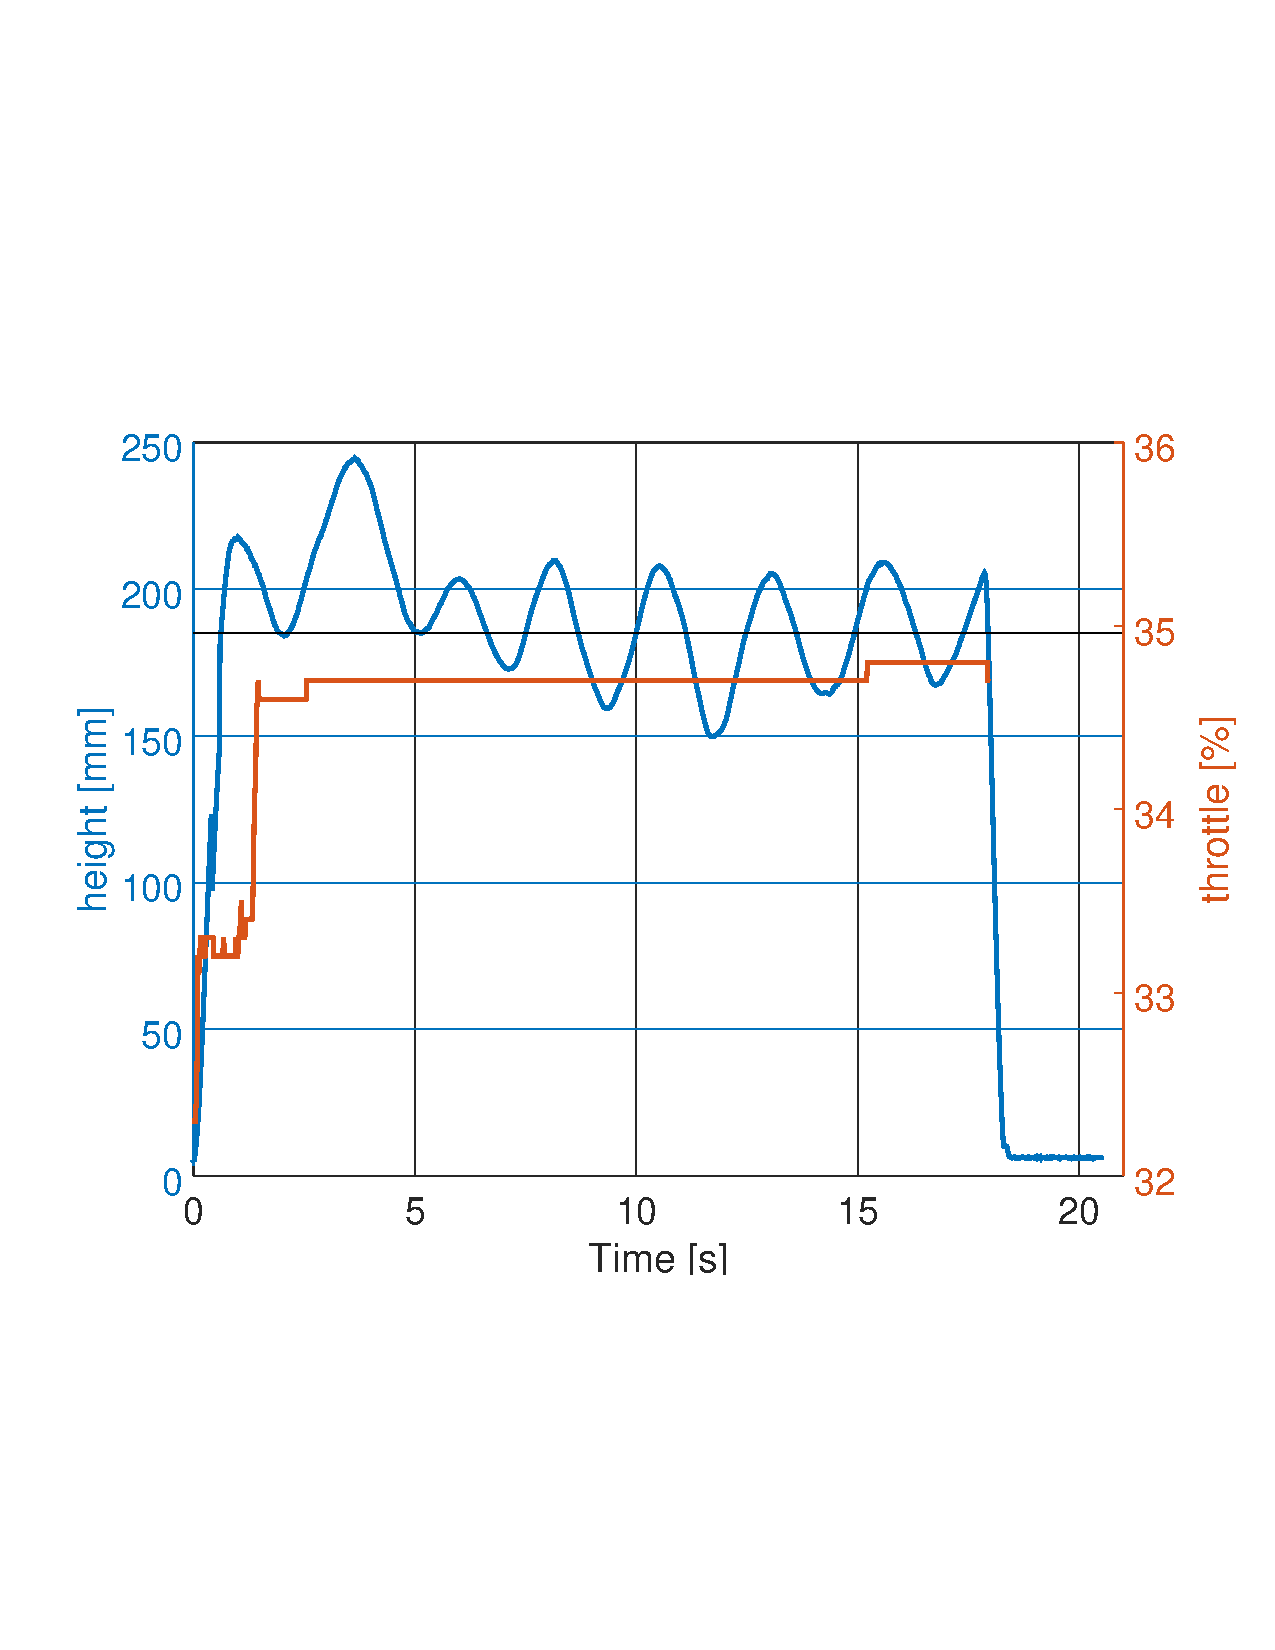
\includegraphics[width=0.6\textwidth, trim={0 7cm 0 7cm},clip]{figures/Appendix/final_test/kp0,012.pdf}
    \caption{Height graph K$_\text{p}$ = 0.01. Marker line is at 185 mm}
    \label{fig:first_test_report}
\end{figure}

From this first test, it was clear the gain was too low. This can be seen by the throttle present only swing with 0.1\% throttle over the gravity offset, on figure \ref{fig:first_test_report}. This is not enough when it is set to make a addition of 100 mm to the height. To compensate for this the K$_\text{p}$ value was set to 0.05, and the test was retried. The result of this test can be seen on figure \ref{fig:second_test_report}.
By making this change to the K$_\text{p}$, the result still did not match the wished result. 
But the result still showed that there were some sort of changing in the throttle present, but still not enough to make the drone raise 100 mm in the height. 
\begin{figure}[H]
    \centering
    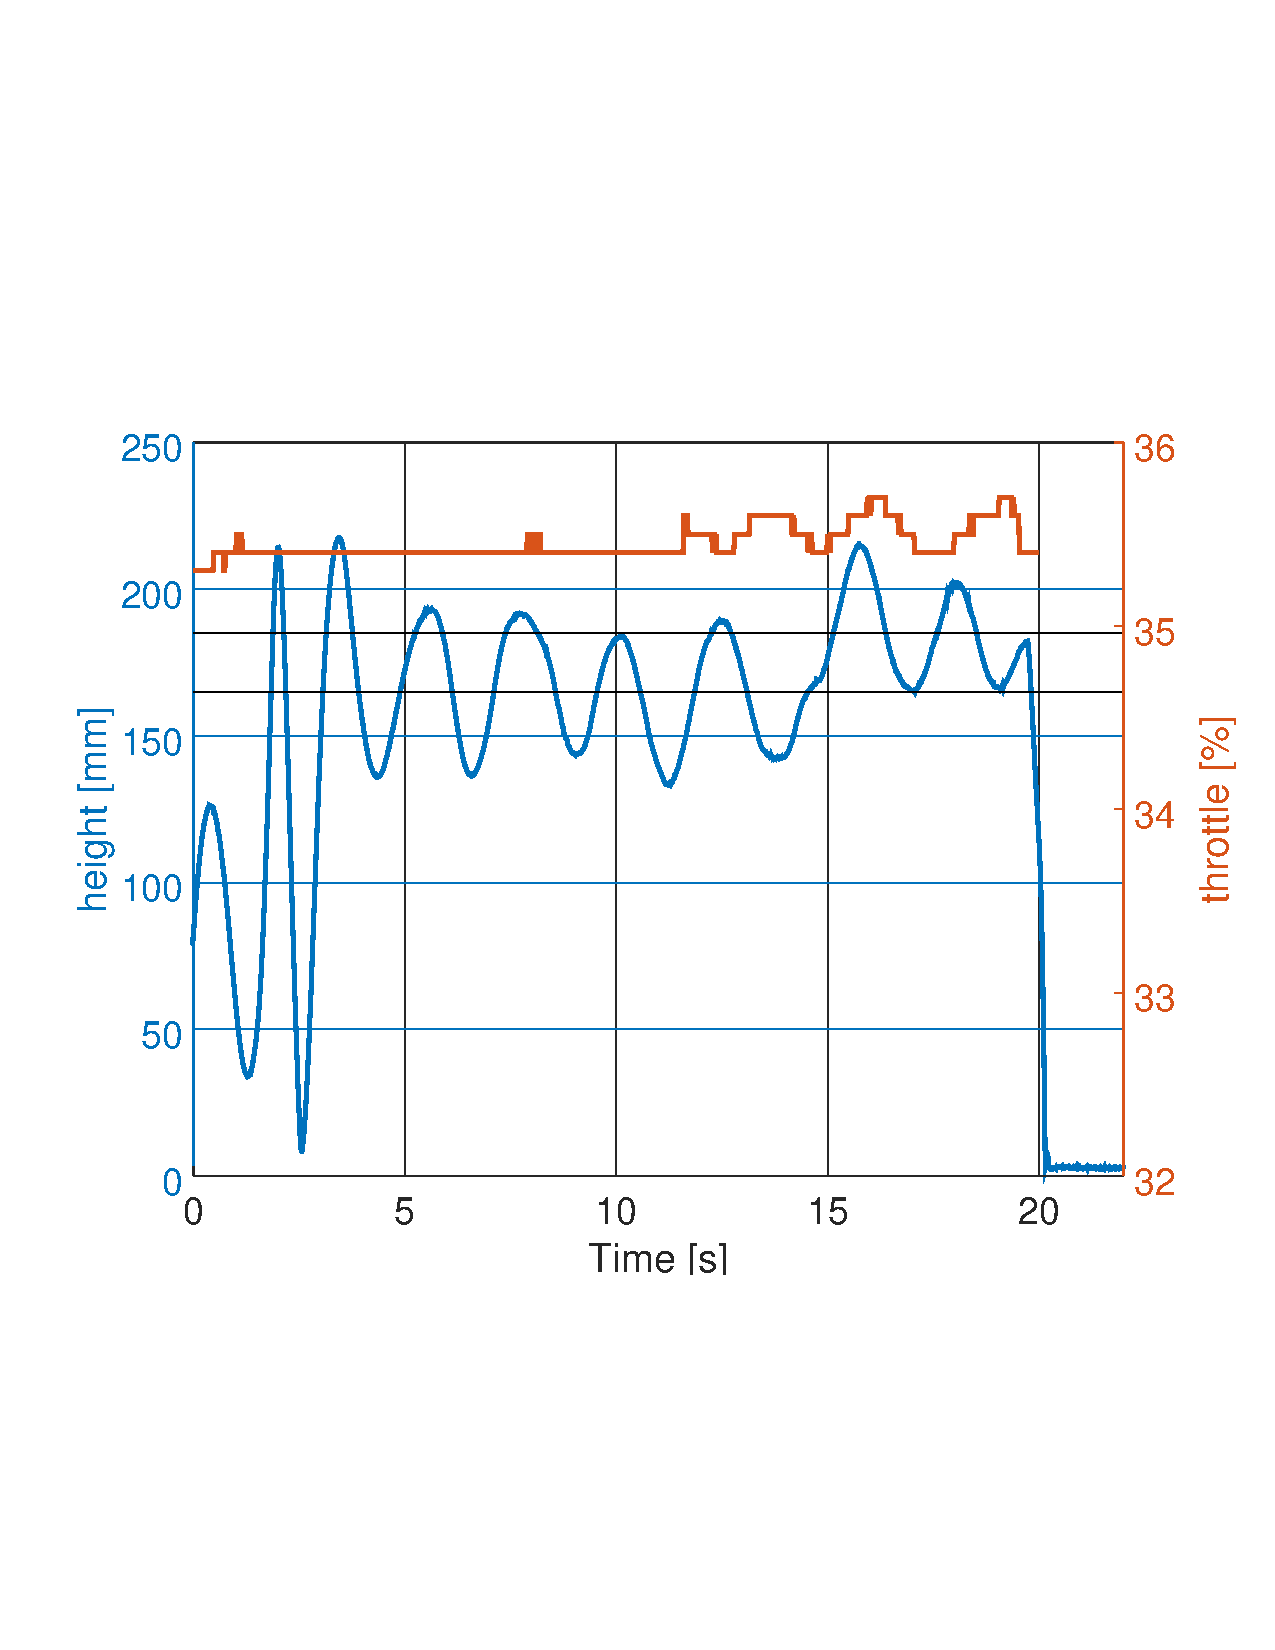
\includegraphics[width=0.6\textwidth, trim={0 7cm 0 7cm},clip]{figures/Appendix/final_test/kp0,05.pdf}
    \caption{Height graph K$_\text{p}$ = 0.05. Marker lines are at 165 and 185 mm}
    \label{fig:second_test_report}
\end{figure}
The K$_\text{p}$ value was further increased, but this gave problems with oscillation, when the K$_\text{p}$ value were set to 0.1, as it can be seen on figure \ref{fig:third_test_report}.
\begin{figure}[H]
    \centering
    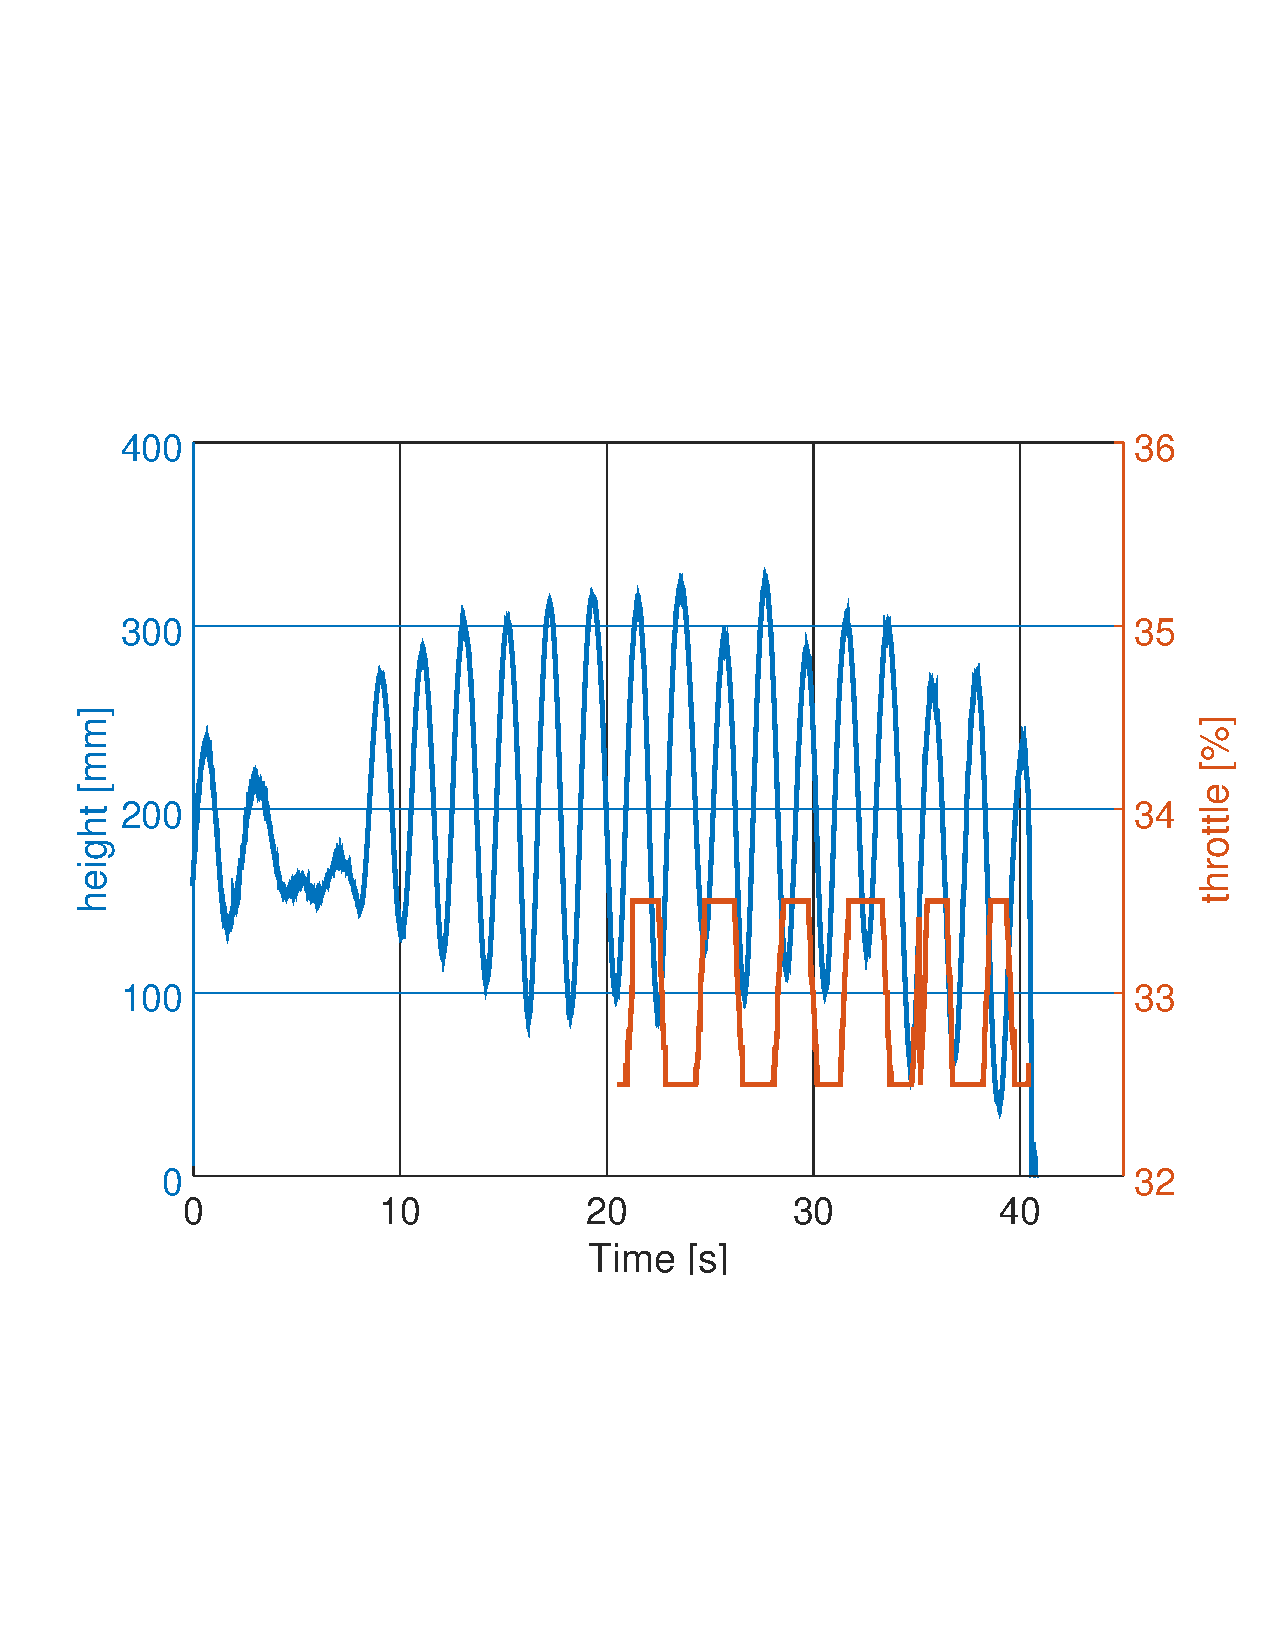
\includegraphics[width=0.6\textwidth, trim={0 7cm 0 7cm},clip]{figures/Appendix/final_test/kp0,1.pdf}
    \caption{Height graph K$_\text{p}$ = 0.1.}
    \label{fig:third_test_report}
\end{figure}

This change in K$_\text{P}$ also highlighted a new issue. In the code, the output throttle was supposed to be limited to 10\% above the offset, which can be seen on figure \ref{fig:third_test_report} the throttle clipped at 1\% swing. This was a simple bug in the code, and once fixed, the results were a bit different. The results without the error in the code can be seen on figure \ref{fig:fourth_test_report}.

\begin{figure}[H]
    \centering
    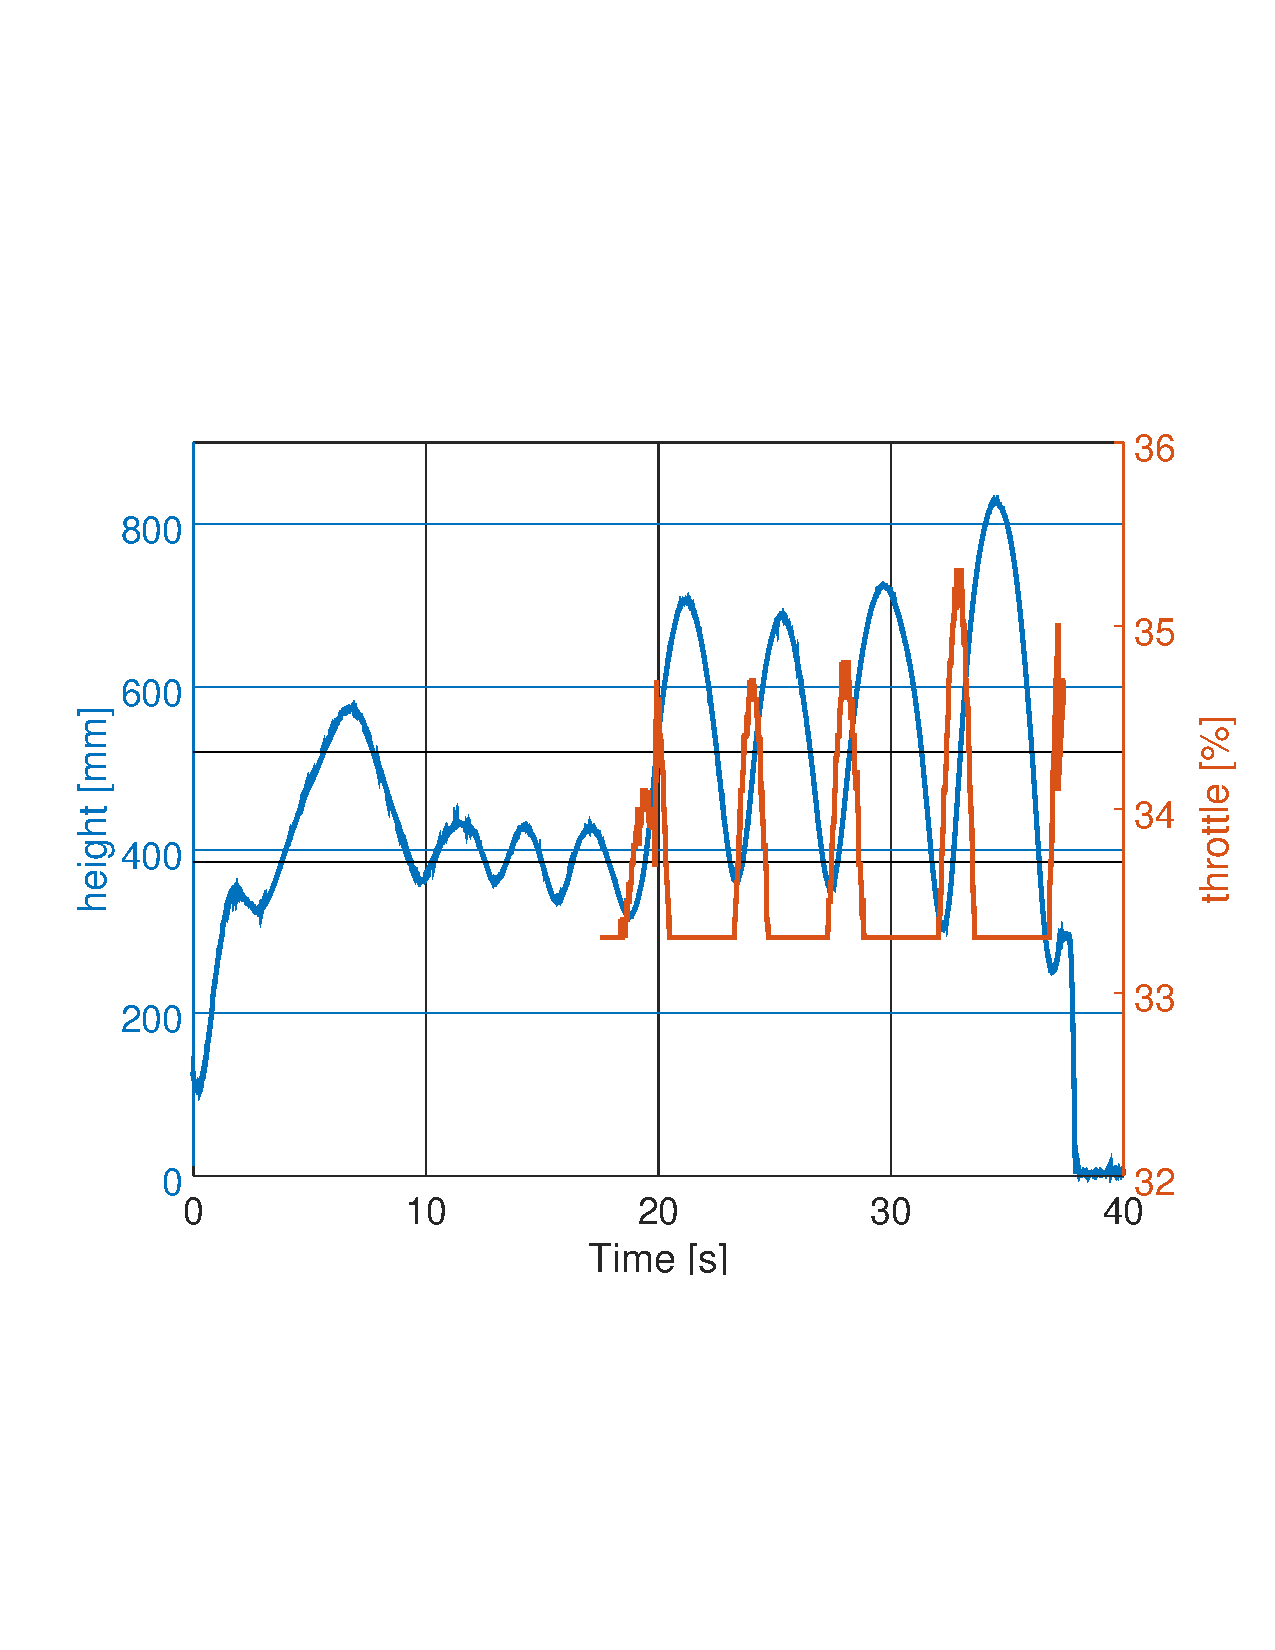
\includegraphics[width=0.6\textwidth, trim={0 7cm 0 7cm},clip]{figures/Appendix/final_test/kp0,1fix.pdf}
    \caption{Height graph K$_\text{p}$ = 0.1 with fixed saturation. Marker lines are at 385 and 520 mm}
    \label{fig:fourth_test_report}
\end{figure}

From the test result on figure \ref{fig:fourth_test_report} it can be seen that the system behaves as it should, when the set point is set 100 mm higher, the system regulates the throttle present to reach this height. The only problem with these results is the high overshoot is gives. and it is oscillating.

\subsection*{Conclusion for the final test}
As a conclusion for the final test, is that the system actually behaves as wanted. The only problem with the test is the high overshoot and oscillation. This problem might have to do with the addition of the K$_\text{p}$ value, this can have a influence on the overshoot and oscillation. So if the time had been to make the first tests again after figuring the fail in the code out, the oscillation and overshoot might have been avoided.

 The excessive oscillations and overshoot is due to the poor phase margin caused by the increased K$_\text{p}$ as can be seen on figure \ref{fig:bodeplot_final} Solutions to this will be discussed in the next chapter.

\begin{figure}[H]
    \centering
    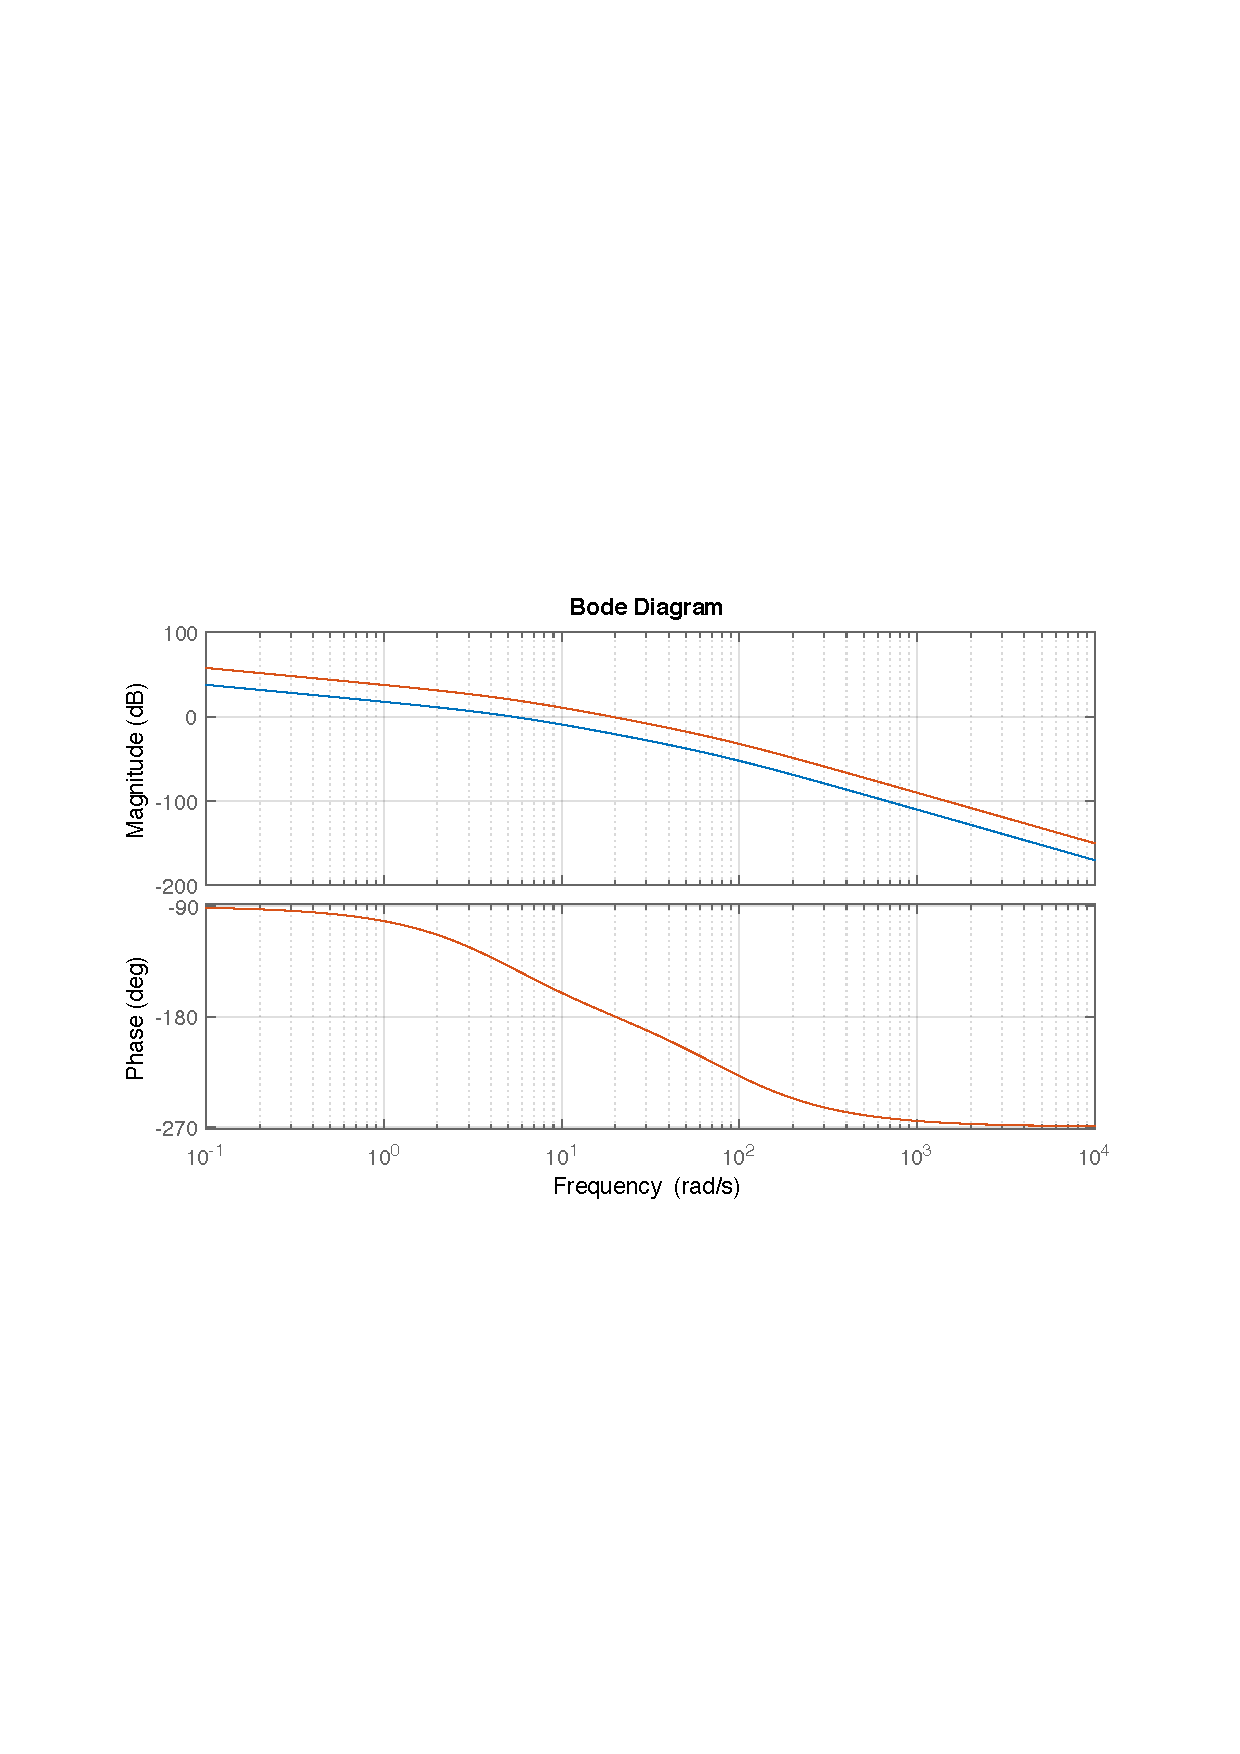
\includegraphics[width=\textwidth]{figures/Appendix/final_test/bodeplot_final.pdf}
    \caption{Bode plot for both the last tested K$_\text{p}$ on 0.1 and the calculated K$_\text{p}$ on 0.01.}
    \label{fig:bodeplot_final}
\end{figure}
\chapter{Discussion}
    The system developed during the project has less than desired performance, and has room for improvement. The poor overshoot performance and the oscillations of the system could be caused by multiple different sources of error. It could be due to an error in our transfer function for the drone. Or due to non-linearity in the thrust of the drone versus the height of the drone, or errors in the code comprising the regulator.\\
Due to these sources of error we decided to perform a new step-response test, and got the results as seen in the test report in appendix \ref{ap:drone_secondary_test}.
As described, the main difference of this step-response test, was that the step was performed at a height above 400 mm. This was because a significant increase in thrust was observed before, when the drone was closer to the floor, and increasing the altitude of the step response would eliminate this effect.


During this test we discovered that the drone would in fact hover at 35\% throttle, the value we had used for the initial step-response test.
This prompted us to reconsider the model of the drone, leading us to believe we had made a mistake in the making of the transfer function for the drone. This was because the step response we were observing in this new test was a constant acceleration, where the previous step we saw would settle on a constant velocity.
Considering this, we tried to model a new transfer function, based on the freebody equation (eq. \ref{eq:new_tf_newton}) for our system, the free body diagram can be seen on figure \ref{fig:Dis_QC_freeBodyDiagram}. 

\begin{figure}[H]
    \centering
    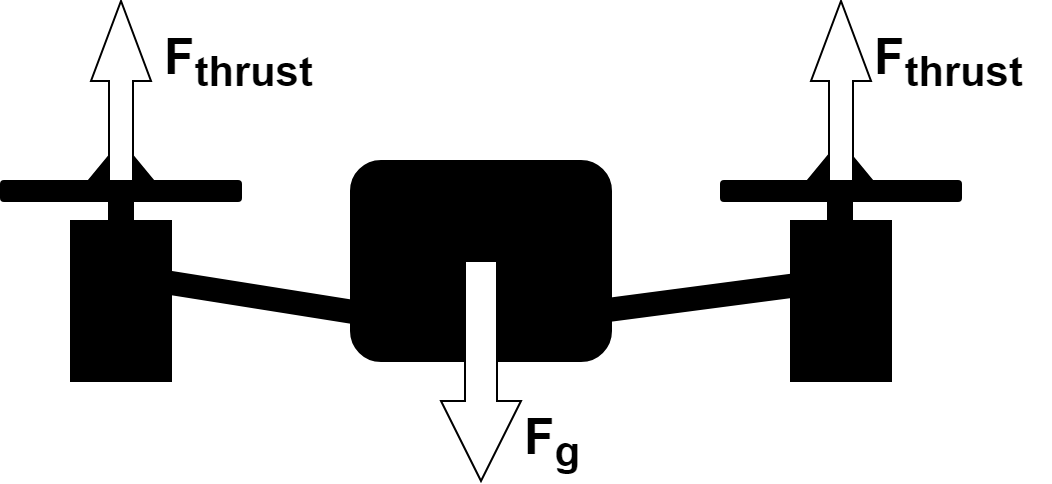
\includegraphics[width=0.45\textwidth]{figures/ch_intro/droen_frit_legeme-diagram.png}
    \caption{Free body diagram of a quadcopter.}
    \label{fig:Dis_QC_freeBodyDiagram}
\end{figure}

\begin{equation} \label{eq:new_tf_newton}
    M_{drone} \cdot \ddot{z} = F_{thrust} - M_{drone} \cdot g
\end{equation}

Where:
\begin{itemize}
    \item $M_{drone}$ is the mass of the drone
    \item $z$ is the vertical position of the drone
    \item $F_{thrust}$ is the vertical thrust generated by the drone
    \item $g$ is the acceleration of gravity
\end{itemize}

Linearizing this transfer function yields equation \ref{eq:new_lin_tf}.

\begin{equation} \label{eq:new_lin_tf}
    \hat{F_{thrust}} = M_{drone} \cdot \ddot{z}
\end{equation}

Laplace transforming this gives us our new equation (eq. \ref{eq:new_zf_laplace}) for the height z.

\begin{equation} \label{eq:new_zf_laplace}
    Z(s) = \hat{F_{thrust}}(s) \cdot \frac{1}{M_{drone} \cdot s^2}
\end{equation}

Yielding us the new transfer function \ref{eq:new_tf} from Thrust to vertical velocity.

\begin{equation} \label{eq:new_tf}
    G(s) = \frac{Z(s)}{\hat{F_{thrust}}(s)} = \frac{1}{M_{drone}} \cdot \frac{1}{s}
\end{equation}

where
\begin{itemize}
    \item $Z(s)$ is the vertical position
    \item $\hat{F_{thrust}}$ is the vertical thrust generated by the drone
    \item $M_{drone}$ is the mass of the drone
\end{itemize}

We believe the cause of the additional lift when the drone is close to the ground, is that the drone creates a cushion of air underneath itself. This cushion causes the drone to generate significantly more thrust when it is close to the ground, causing lower throttle percentages than is required to hover the drone, to accelerate the drone. This was backed up by further tests, showing a 0\% to 35\% throttle step of 1 second would cause the drone to hit the roof of the motion-tracking lab. However by manually saving the thrust when an operator hovered the drone, showed that slowly bringing the drone up to a hover, would have the drone hovering at 35\%.

Because of the above difficulties, this air-cushion has caused a lot of difficulties in developing the controller for the drone. A solution to automatically adjust for this, could be to implement an integral part to the controller. However another issue we struggled with was oscillations due to poor phase margin at the required proportional gain, and an integral part would have further worsened our phase margin. 


As mentioned we struggled with oscillations when testing the drone. These were a result of increased Kp, as the initially calculated Kp was too small to give any noticeable throttle output, and after increasing it, we observed excessive oscillation around the set points. We also noticed during testing, that the throttle saturated too early due to a firmware error, but what we failed to see, was that the throttle output also saturated too early on the negative swing. Fixing this might have decreased the oscillations on figure \ref{fig:fourth_test_report}, as it would have allowed the drone to decelerate faster.


Another solution for decreasing the oscillations of the drone, could be to implement a PD controller instead of just a P regulator, as the derivative part would increase the phase margin of the system at higher gains, and damp oscillations.

When we noticed the oscillations, we decided to verify that the sensors sampled at the assumed sample-rate.\\
Due to a bug in the library used to communicate with the sensors, the desired method of interrupt driven sensor sampling was not possible, and we had to resort to polling the sensors instead. This worked surprisingly well as can be seen on figure \ref{fig:sample_test}.

\begin{figure}[H]
    \centering
    \makebox[\textwidth][c]{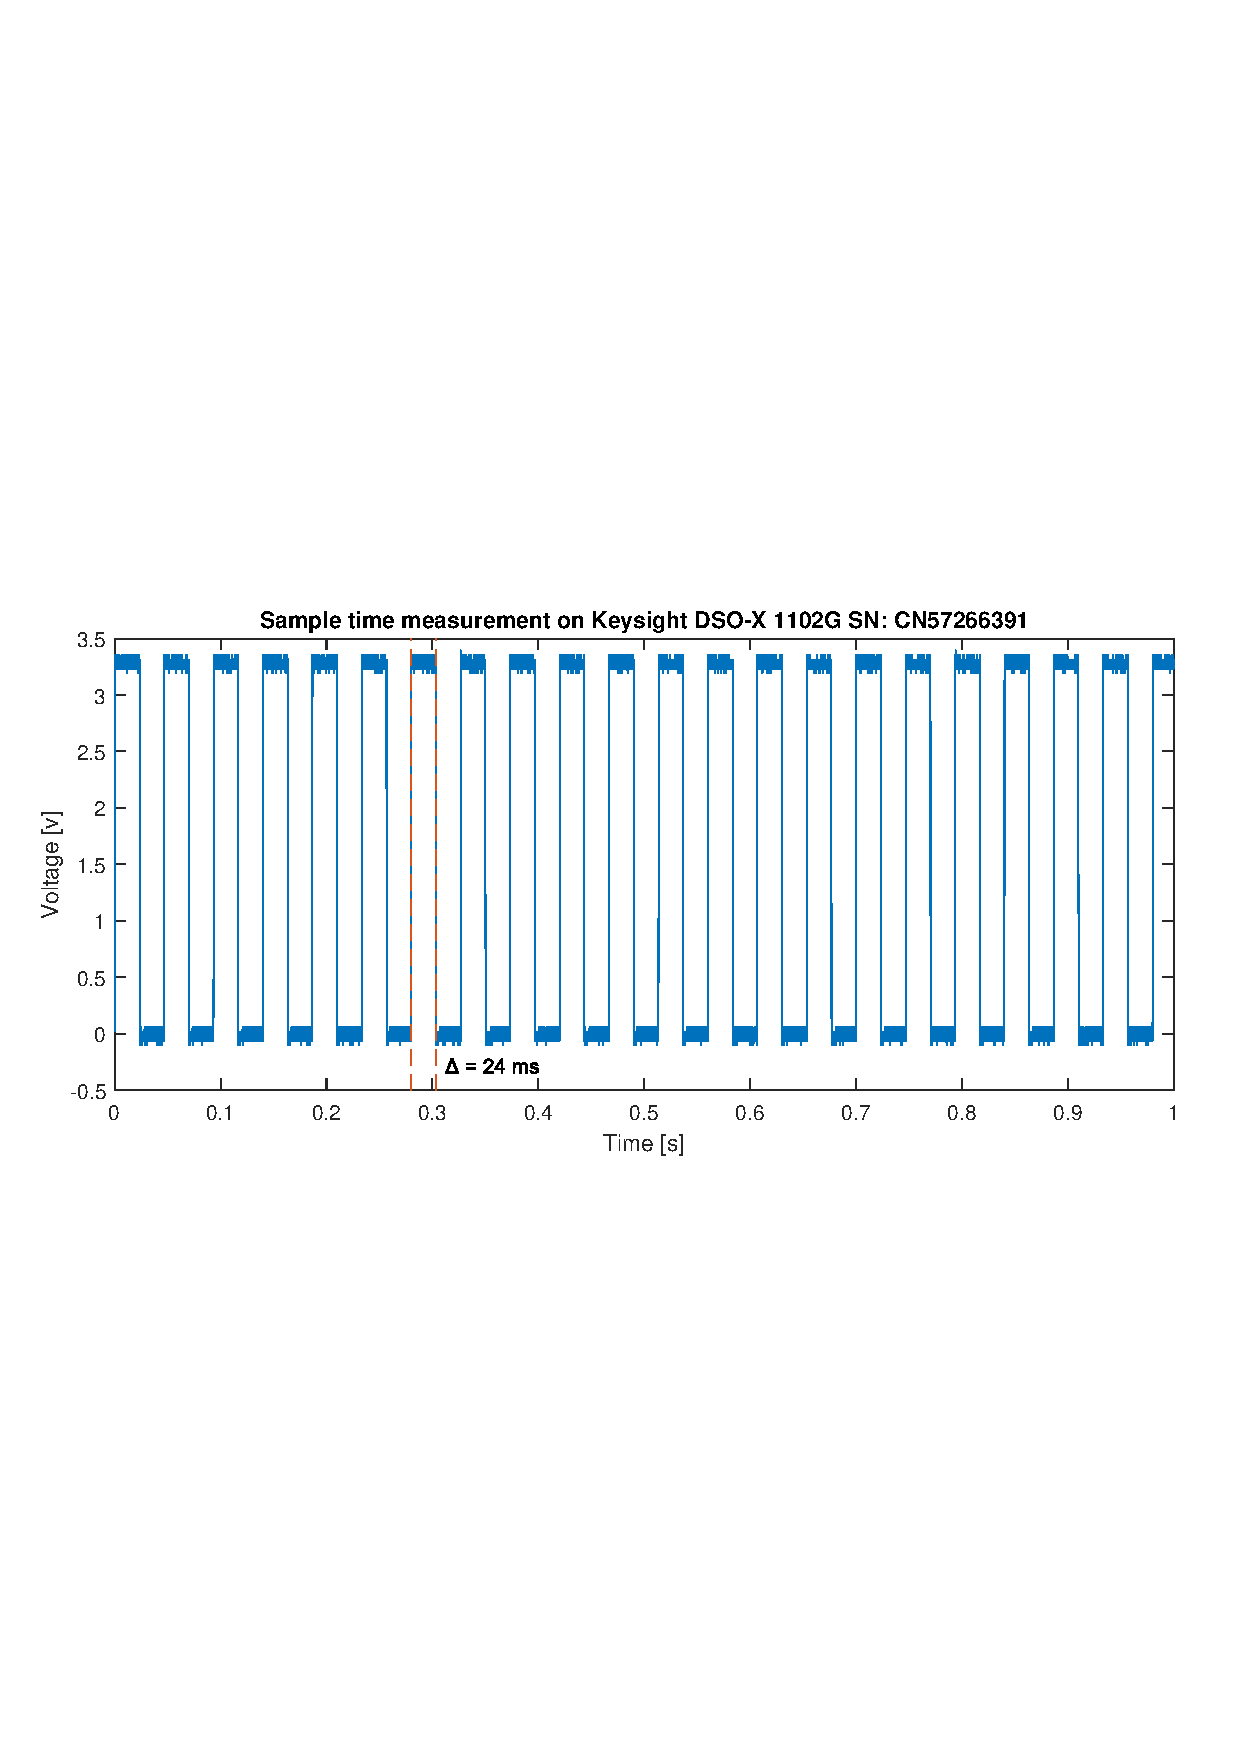
\includegraphics[width=1.2\textwidth, trim={0 9.5cm 0 9.5cm},clip]{figures/scope.pdf}}
    \caption{Capture of pin-toggles every time the sensor is sampled}
    \label{fig:sample_test}
\end{figure}

A small addition was added to the code, where it would invert a debug pin every time the sensor was sampled. This pin was then captured using a DSO, with the motors of the drones spinning at high speed to generate noise on the logic supply, and simulate flight. As can be seen, the sample-time was reliably 24 ms, with virtually no jitter in sample rate. This means our discretization of the sensor is still valid.

Another possible error we did not test due to time constraints, was how the sensors distance readings performed at 400 mm distance, in flying conditions. We did consider saving these data, but the code already used the majority of the EEPROM to save the throttle data, and we did not have any options to communicate with the drone-shim wirelessly.
Had time allowed it, a possible feature could have been added to the drone, keeping 1000 samples of height data in a ring buffer in RAM, as we still had plenty of RAM spare. 

























    \newpage
\chapter{Conclusion}
    The project documents how to develop a system to maintain an off-the-shelf drone a fixed distance from

As discussed in the discussion the system does not fulfill all the requirements for the system. The requirements that where not fulfilled are the overshoot for the system, the settling time, steady state. 
The requirement for the overshoot can not be met doing to the model of the drone might have been determined the wrong way. This has also an infect on the settling time and the steady state, mostly because of the d
Resultatet fra diskutionen

Kravene

    

%\chapter{Simulations}
    %\section{Simulations}

%
%

%%%%%%%%% Unsorted things %%%%%%%%%

% \chapter{Template examples}
%     \section
%         Well, like this
\subsection{This is a Subsection}
and this
\subsubsection{This is a Subsubsection}
and this.

\paragraph{A Paragraph}
You can also use paragraph titles which look like this.

\subparagraph{A Subparagraph} Moreover, you can also use subparagraph titles which look like this\todo{Is it possible to add a subsubparagraph?}. They have a small indentation as opposed to the paragraph titles.

\todo[inline,color=green]{I think that a summary of this exciting chapter should be added.}
%     \section{Place Holders}\label{ch:place_holders}
%         How do you use placeholders?

This is how you use placeholder figures
\missingfigure{We need a figure right here!}
%     \section{Conclusion}\label{ch:conclusion}
%         The project documents how to develop a system to maintain an off-the-shelf drone a fixed distance from

As discussed in the discussion the system does not fulfill all the requirements for the system. The requirements that where not fulfilled are the overshoot for the system, the settling time, steady state. 
The requirement for the overshoot can not be met doing to the model of the drone might have been determined the wrong way. This has also an infect on the settling time and the steady state, mostly because of the d
Resultatet fra diskutionen

Kravene


%
% Bib stuff
\printbibliography[heading=bibintoc]
\label{bib:mybiblio}
\appendix
%\chapter{Appendix A name}\label{ch:appAlabel}
Here is the first appendix
\chapter{Test of a sensor}\label{ap:testOfSensors}

%
%\section*{Purpose}
%The purpose of this test is to analyze the accuracy of the sensor\todo{navnet på sensor} at specific distances, as well as determine the sampling rate.
The purpose of this test is to examine the VL53l0X sensor, to see if the sensor meets the following requirement from chapter \ref{ch:Req}:
\begin{itemize}
    \item Detect a wall from minimum 1 meter.
    \item Accuracy of $\pm$5 \% at 400 mm.
    \item sampling rate of 40 Hz
    \item detection of wall with a angle of 0$\degree$ $\pm 10 \degree$
\end{itemize}
The examination of the VL53l0X sensors will be done in two test, one to determined the sensors accuracy and highest possible distance to a wall. Secondly there will be tested if it's possible for the VL53l0X sensors to detect the wall with a angel of $\pm 10 \degree$.
The VL53l0X sensors uses i2C to communicate.

%
\section*{Test setup}
The test will be executed with a custom made breakout board to an Arduino Uno, which interfaces two VL53l0X sensors to the arduino. The VL53l0X sensors are placed a specific distance from a white wall. This setup is illustrated in figure \ref{fig:testSetupSensor}.
\begin{figure}[H]
    \centering
    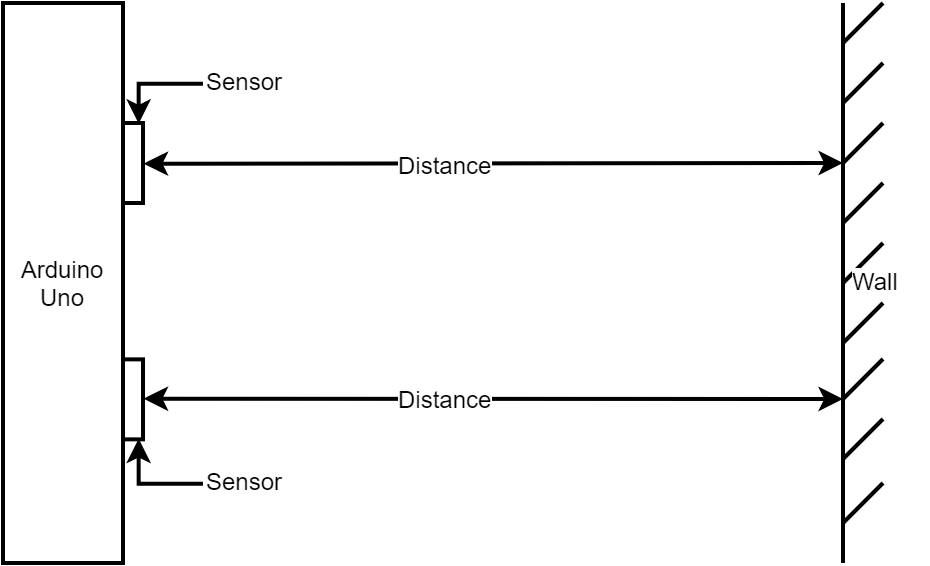
\includegraphics[width=0.6\textwidth]{figures/Appendix/testopstillingSensor.png}
    \caption{Illustration of the test setup.}
    \label{fig:testSetupSensor}
\end{figure}

%
\section*{Execution}
The code used to test the sensors can be found in the github repository \url{https://github.com/AAU-EIT5/VL53L0X-sensor-test}. The code is getting a 100 readings from the sensor, and then printing them out in the arduino monitor.
\newline
The first test are executed by taking readings with the sensors from different distances, starting from 30 cm and ending at 110 cm, with a interval of 10 cm between each. The distances a measures with a measuring tape.
\newline
The second test are executed at a distance of 110 cm, where the sensor broad is with the angel +10$\degree$ and -10$\degree$. 

%
\section*{Results}
For the first test can the results for sensor 1 can be seen on figure \ref{fig:resultatSensor1test} and for sensor 2 in figure \ref{fig:resultatSensor2test}. The average time the sensors took to measure a 100 values at adjusted time of 20 ms is 1848961 microseconds, which approximately equals to 18.5 milliseconds, that gives a sampling rate of 54 Hz. 

\begin{figure}[H]
    \centering
    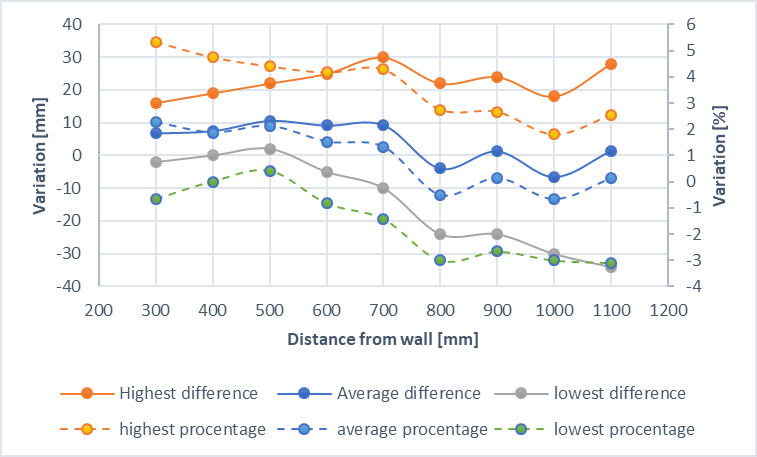
\includegraphics[width=0.8\textwidth]{figures/Appendix/resultatSensor1Test.png}
    \caption{Results from sensor 1.}
    \label{fig:resultatSensor1test}
\end{figure}
\begin{figure}[H]
    \centering
    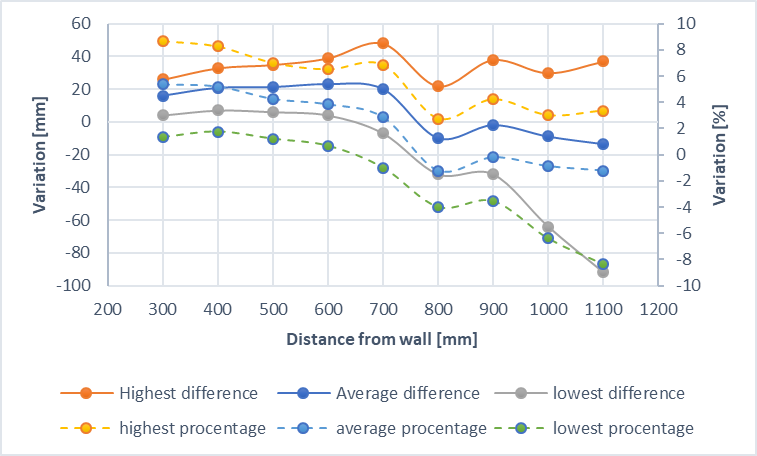
\includegraphics[width=0.8\textwidth]{figures/Appendix/resultatSensor2Test.png}
    \caption{Results from sensor 2.}
    \label{fig:resultatSensor2test}
\end{figure}

The results from the test to see if the sensors could detect a wall when it have a angel of $\pm 10 \degree$ can be seen in table \ref{tab:sensorAngelRes}.
\begin{table}[H]
    \centering
    \caption{Results from test of sensors with a angle of $\pm 10 \degree$.}
    \label{tab:sensorAngelRes}
    \begin{tabular}{|c|c|c|}
    \hline
             & \textbf{10$\degree$ left} & \textbf{10$\degree$ Right}  \\ \hline
    \textbf{Results sensor 1:} & Detected in all readings  & Detected in all readings    \\ \hline
    \textbf{Results sensor 2:} & Detected in all readings  & Detected in all readings    \\ \hline
    \end{tabular}
\end{table}

%
\section*{Discussion}
From figure \ref{fig:resultatSensor1test} and \ref{fig:resultatSensor2test} can it be seen that the sensors can detect a wall that are at lest op to 1100 mm. As one of the requirements the sensors have to hold are a detection of a wall at minimum 1000 mm, do the sensors comply with this requirement.
\newline
\newline
Another requirement the sensor have to comply is a accuracy of $\pm 10 \degree$ at 400 mm distance from a wall. If figure \ref{fig:resultatSensor1test} can there be notice a variation of around 0 $\%$ to around 5 $\%$ from the actual distance and as the requirement for the sensors is $\pm 5 \%$, sensor 1 comply with it. On the other hand, do sensor 2 not comply with the requirements, as it's variation a 400 mm is from around 1 $\%$ to around 9 $\%$, but as it can be observed from the figures \ref{fig:resultatSensor1test} and \ref{fig:resultatSensor2test}, are the averages measurements both shifted from the actually distance from the wall. If the shifted distance are taking into account, are the accuracy of both sensors with ind the required accuracy. 
\newline
\newline
Some of the factors that can cause the shifting of the distance, is firstly the measured distance with measuring tape the sensors where placed can be inaccurate with a few millimeters. secondly the board the sensors where on could have a slight angle, there one sensor then would be closer to the wall than the other. lastly the sensors measuring can be off, when initializing the sensors.
\newline
\newline
The third requirement the sensors have to abide are a sampling rate of a 40 Hz, and as the measured sampling rate of the sensors are 54 Hz, meets the sensors the requirement. As the sensors where set to a sampling rate of 50 Hz, can the difference of 4 Hz be because of the sensors where faster to get a reading than enlightened from the datasheet.
\newline
\newline
Lastly a requirement for how high a angel the sensors have to detect the wall was set $\pm 10 \degree$, where both sensors could detect them a 1100 mm distance. Some of the uncertain factors for this test, are the precise angle of the board, as it could variate a couple of degrees. The exact distant could also vary a couple of mm, but as the measured distance to the wall was lager than 1 meter this have no influence of the results.

%
\section*{Conclusion}
From the results of the test, can there be concluded whether the sensors comply with the requirements. the first requirements the sensor have to comply with are the detection of a wall of 1 meter, and as it can detect the wall a 1.1 meter distance it meets with the requirement.
\newline
The second requirement the sensor have to comply are a accuracy of $\pm 5 \%$ at 400 millimeters, that it only meets of the shifted distance of the sensors, where it then have a a accuracy of op to $\pm 4 \%$.
\newline
The third requirement the sensors have to meet are a sampling rate of 40 Hz, that it meets as it can have a sampling rate op to 54 Hz.
The last requirement the sensor have to meet are the angle of $\pm 10 \degree$ which the sensors have to detect, and from the test it can be seen that i sensors can detect the wall at this distance.
\newline 
Over all are all the requirements meet with the sensors, if the shifting of the distance are taking into account. 
\chapter{Drone flight measuring test}\label{ap:drone_flight_test}
The purpose of this test is to get a model of how the drone are moving in upward movements, and to make a function of the behaviour. The test will be performed in the Motion detection Lab, located in room  at AAU, where the Vicon system \ref{s:vicon} is placed. The reason for using this system is because it can track an object's position in all x, y and z-axis at the same time. From this data it will be possible to make a model of the drone's movements and from that make the transfer function.

\section*{Test setup}
The components there are used in the test are as the following point:
\begin{itemize}
    \item{Vicon system}
    \item{Reflectors}
    \item{Drone}
    \item{Teensy 3.2} % navnet på micro kontrolene
    \item{Turnigy TGY-iA6} % navn på reciver
    \item{Turnigy TGY-A6} % navn på transmitter
\end{itemize}
For the Vicon tracking system to track the drone, five reflectors is set on the drone. The placement of the reflectors can be seen in figure \ref{fig:reflectors}.
The drone are placed in the room with the Vicon cameras. Where the Vicon system can record the drones movement, by tracking the reflectors. 

\begin{figure}[H]
    \centering
    \includegraphics[width=0.4\textwidth]{figures/Appendix/measuringTest/Reflector1.pdf}
    \caption{Illustration of placement of the reflectors on the drone.}
    \label{fig:reflectors}
\end{figure}


\section*{Execution}
Before the test can be executed, a calibration of the Vicon cameras have to be done. After the Calibration the test code are transferred to the Teensy for controlling the drone. When the Vicon system is set to track the drone by it's reflectors, the drone is then set to fly at a steady level. From this steady level, it is set to run a program, which makes the drone keep a throttle level on 30 \% in 10 seconds, and then raise the level to 33\% in 1 second and then back to 30\% afterwards. The code to run this program can be seen in the Github repository. From this step response it is possible to make a model of the drones movements, and calculate the values for the transfer function. 



\section*{Results}
The data is plotted in the figure \ref{fig:positiontime}, in this figure the plot is directly from the data, which is time and position. In the figure the blue line is the plotted data.

\begin{figure}[H]
    \centering
    \includegraphics[width=0.95\textwidth]{figures/Appendix/measuringTest/DroneTest.png}
    \caption{Plot of the recorded data.}
    \label{fig:positiontime}
\end{figure}

\section*{Discussion}
From this test it can be seen in the data that the requirement of the speed is fulfilled, in the point that it takes more then one second to move one meter in distance. But apart from that there are some problems in how the drone moves before the systems go in and take over, the drone cannot start from the ground. So the drone needs to fly in a steady level, this gives some problems in getting the right data from all the recorded data. From this point the data will be needed to be sorted. To make sure that the plotted data is for the step response and not for the drop after worth and not to long before the drop. 
\newline
Apart from this problem, the data represent movement of the drone, because the movement of the drone is tracked in the Vicon system, so the drone can be followed to make the correct time. The data is therefor the best representation of the movement, so these data will be used for the model of the drone.

\section*{Conclusion}
The data from this it will be possible to make a real model of the drone's movements. Where the data from this test, is only a position in time, therefor the data needs to be changed to a model of the speed over time instead. Apart from this the data plotted in figure \ref{fig:positiontime} shows that the drone fulfill the requirement for the speed and also make a useful foundation for making a model of the drone's movements in a step response.






\chapter{Test of the final system}\label{ap:final_test_report}

The purpose of this test are to examined the final control system implemented on the quadcoptor and see if the system meats the requirements from chapter \ref{ch:Req} in the report. The test has been preformed in the Motion Tracking lab, located at AAU Fredrik Bajers Vej 7 room C2-111, as the Vicon system is located there. 


\section*{Test setup}
The components there are used in the test are as the following point:
\begin{itemize}
    \item{Vicon system}
    \item{Reflectors}
    \item{Drone}
    \item{Teensy 3.2} % navnet på micro kontrolene
    \item{Turnigy TGY-iA6} % navn på reciver
    \item{Turnigy TGY-A6} % navn på transmitter
\end{itemize}
For the Vicon tracking system to track the drone, five reflectors is set on the drone. The placement of the reflectors can be seen in figure \ref{fig:reflectors_final_test}.
The drone are placed in the room with the Vicon cameras. Where the Vicon system can record the drones movement, by tracking the reflectors. 

\begin{figure}[H]
    \centering
    \includegraphics[width=0.3\textwidth]{figures/Appendix/measuringTest/Reflector1.pdf}
    \caption{Illustration of placement of the reflectors on the drone.}
    \label{fig:reflectors_final_test}
\end{figure}

To make the final test of the quadcoptor, the control system found in chapter \ref{ch:design_control_sys} has been programmed for the Teensy on the drone. The program for the Teensy can be fiound in the github repository \url{https://github.com/AAU-EIT5/drone-shim}.

\section*{Execution}
As discussed in section \ref{sec:control_code}, the drone has to be manually flown to the point where it hovers. Here the pilot flips a switch to set the gravity offset thrust, and set the initial set-point. If the operator flips the switch to the next position, 100 mm is added to the set point.

This was the procedure used in the motion tracking lab, and the drone was tracked using the Vicon system to track its height over time. Additionally code was added that tracked the demanded throttle every 20ms, and once the aforementioned switch was returned to it's initial position, would save the last 20 seconds of these samples to EEPROM on the micro-controller. This would then be output on power-up over serial, when the drone was connected to a PC.

\section*{Results}
The resulting height data and throttle data can be seen on figure \ref{fig:first_test}

\begin{figure}[H]
    \centering
    \includegraphics[width=0.9\textwidth, trim={0 7cm 0 7cm},clip]{figures/Appendix/final_test/kp0,012.pdf}
    \caption{Height graph Kp = 0.012. Marker line is at 185 mm}
    \label{fig:first_test}
\end{figure}

From this first test, it was clear that our gain was too low, as the regulator only produced a maximum output swing of 0.1\% throttle over the gravity offset. because of this we tuned the gain from 0.012 to 0.05, and performed a second test. The result of this test can be seen on figure \ref{fig:second_test}.
With this test, we still didn't see the expected result from the regulator, so we further increased Kp to 0.1 and discovered a new problem.

\begin{figure}[H]
    \centering
    \includegraphics[width=0.9\textwidth, trim={0 7cm 0 7cm},clip]{figures/Appendix/final_test/kp0,05.pdf}
    \caption{Height graph Kp = 0.05. Marker lines are at 165 and 185 mm}
    \label{fig:second_test}
\end{figure}

\begin{figure}[h]
    \centering
    \includegraphics[width=0.9\textwidth, trim={0 7cm 0 7cm},clip]{figures/Appendix/final_test/kp0,1.pdf}
    \caption{Height graph Kp = 0.1.}
    \label{fig:third_test}
\end{figure}

\begin{figure}[h]
    \centering
    \includegraphics[width=0.9\textwidth, trim={0 7cm 0 7cm},clip]{figures/Appendix/final_test/kp0,1fix.pdf}
    \caption{Height graph Kp = 0.1 with fixed saturation. Marker lines are at 385 and 520 mm}
    \label{fig:fourth_test}
\end{figure}


The regulator is limited in code to saturate early in order to avoid an improperly tuned regulator from crashing the drone, as full throttle is far too high for our drone, and especially for use inside. However the new Kp highlighted a problem with this limiting, as seen on figure \ref{fig:third_test}. The limiting was supposed to be 10\%, but as the code works in steps of 0.1\% it was mistakenly set to 1\% This was corrected, and the behaviour seen on figure \ref{fig:fourth_test} was observed. In this test we achieved closer to what we had expected, but we do see significant oscillations, and high overshoot.
It can all be seen on figure \ref{fig:second_test}, \ref{fig:third_test} and \ref{fig:fourth_test} that error in the program have been made so the throttle could not get under the hover throttle. This problem could increase the overshoot so the system could not stabilize the Quadcoptors height.

\section*{Conclusion}
From the data collected in the test, it can be seen the original calculated Kp factor was to small to increase the the height of the drone. By increasing the Kp factor the system increases it height of the quadcoptor but also increases the overshoot and oscillation.
From the test there was also found a error of the throttle limits in the program which contributes to the oscillation and high overshoot.
\chapter{Secondary test of step response}\label{ap:drone_secondary_test}
The purpose of this test is to get a model of how the drone are moving in upward movements, and to make a function of the behaviour. The test will be performed in the Motion detection Lab, located at AAU Fredrik Bajers Vej 7 room C2-111, where the Vicon system \ref{s:vicon} is placed. The reason for using this system is because it can track an object's position in all x, y and z-axis at the same time. From this data it will be possible to make a model of the drone's movements and from that make the transfer function.

\section*{Test setup}
The components there are used in the test are as the following point:
\begin{itemize}
    \item{Vicon system}
    \item{Reflectors}
    \item{Drone}
    \item{Teensy 3.2} % navnet på micro kontrolene
    \item{Turnigy TGY-iA6} % navn på reciver
    \item{Turnigy TGY-A6} % navn på transmitter
\end{itemize}
For the Vicon tracking system to track the drone, five reflectors is set on the drone. The placement of the reflectors can be seen in figure \ref{fig:reflectors_secondary}.
The drone are placed in the room with the Vicon cameras. Where the Vicon system can record the drones movement, by tracking the reflectors. 

\begin{figure}[H]
    \centering
    \includegraphics[width=0.4\textwidth]{figures/Appendix/measuringTest/Reflector1.pdf}
    \caption{Illustration of placement of the reflectors on the drone.}
    \label{fig:reflectors_secondary}
\end{figure}

\section*{Execution}
Before the test can be executed, a calibration of the Vicon cameras have to be done.After the Calibration the test code are transferred to the Teensy for controlling the drone. The drone will be manually flown by the pilot up to a height far enough away from the floor where it hovers without the help of the air-cushion it generates close to the ground. This is >400 mm more then from the floor, this is done to get out of the air pillow that get created underneath the drone when it begins to fly, because the air pillow have some infect on the step response else. When the drone is hovering the step can start, so the drone will go to a throttle value of ?? in ?? second. After this time the drone will increase the throttle value to ?? in ?? second and after this second the drone will go back to hovering. The whole step response is tracked and recorded using the Vicon system and the reflectors on the drone.


\section*{Results}
From the Vicon system the result from the step response are plotted using MatLab. The plot can be seen on figure \ref{fig:secondary_stepresponse}.
\begin{figure}
    \centering
    \includegraphics{figures/Placeholder.png}
    \caption{Plot of the step response made using the tracked data from Vicon.}
    \label{fig:secondary_stepresponse}
\end{figure}

From the data it can be seen, that the response is looking more like a first order transfer function, because it has a more linear behavior, which is a fundamental element for a first order transfer function. A first order transfer function is based on the equation \ref{eq:first_order}.
\begin{equation}\label{eq:first_order}
    G(s)=\frac{1}{sT}
\end{equation}
To get the closed loop control system from this equation \ref{eq:first_order}, there are some assumption that needs to be taken, first the system has a output C(s) and an input R(s), then the equation \ref{eq:closed_loop_first}.
\begin{equation}\label{eq:closed_loop_first}
    \frac{C(s)}{R(s)}=\frac{G(s)}{1+G(s)} \to \frac{C(s)}{R(s)}= \frac{\frac{1}{sT}}{1+\frac{1}{sT}}=\frac{1}{sT+1}
\end{equation}
This equation is a closed loop transfer function for a first order system \cite{digital_control}. 




















\end{document}